%%%%%%
% vr-thesis-template.tex
%%%%%%%

% Import preamble settings
% Document class
\documentclass[fontsize=12pt, paper=a4, headinclude, twoside=false, parskip=half+, pagesize=auto, numbers=noenddot, plainheadsepline, open=right, toc=listof]{scrreprt}

% PDF compression
\pdfminorversion=5
\pdfobjcompresslevel=1

% General
\usepackage[automark]{scrpage2}          % Header and Footer
\usepackage{amsmath, marvosym}           % Math libraries
\usepackage[utf8]{inputenc}              % UTF8-Encoding
\usepackage{amsthm}
\usepackage[bottom]{footmisc}

% Font
\usepackage{mathpazo}                    % Palatino for math
\usepackage{setspace}                    % Line space
\onehalfspacing                          % Line space 1.5
\setkomafont{chapter}{\Huge\rmfamily}    
\setkomafont{section}{\Large\rmfamily}
\setkomafont{subsection}{\large\rmfamily}
\setkomafont{subsubsection}{\large\rmfamily}
\setkomafont{chapterentry}{\large\rmfamily}
\setkomafont{descriptionlabel}{\bfseries\rmfamily}
\setkomafont{captionlabel}{\small\bfseries}
\setkomafont{caption}{\small}
\usepackage{amssymb}
\usepackage{tcolorbox}

% Language: German
\usepackage[german]{babel}

% PDF-Output
\usepackage[german, colorlinks=false, linkcolor=black]{hyperref}
\usepackage[final]{microtype}
\usepackage{url}
\usepackage{pdflscape}

% Tables
\usepackage{multirow}
\usepackage{multicol}
\usepackage{tabularx}
\usepackage{array}
\usepackage{float}
\usepackage{varwidth}
\usepackage{verbatimbox}

% Images
\usepackage{graphicx}
\usepackage{color}
\graphicspath{{images/}}
\DeclareGraphicsExtensions{.pdf,.png,.jpg}
\usepackage{subfigure}
\newcommand{\subfigureautorefname}{\figurename}
\usepackage[all]{hypcap}
\setcapindent{0em}
\setcapwidth[c]{0.9\textwidth}
\setlength{\abovecaptionskip}{0.2cm}

% Source code
\usepackage{listings}

\definecolor{mygreen}{rgb}{0,0.6,0}
\definecolor{mygray}{rgb}{0.5,0.5,0.5}
\definecolor{mymauve}{rgb}{0.58,0,0.82}

\lstset{ %
  backgroundcolor=\color{white},   % choose the background color
  basicstyle=\scriptsize\ttfamily,        % size of fonts used for the code
  breaklines=tduringrue,                 % automatic line breaking only at whitespace
  captionpos=b,                    % sets the caption-position to bottom
  commentstyle=\color{mygreen},    % comment style
  escapeinside={\%*}{*)},          % if you want to add LaTeX within your code
  keywordstyle=\color{blue},       % keyword style
  stringstyle=\color{mymauve},     % string literal style
  frame=single
}

% Quotes
\usepackage{epigraph}
\setlength\epigraphwidth{10cm}
\setlength\epigraphrule{0pt}
\usepackage{etoolbox}
\makeatletter
\patchcmd{\epigraph}{\@epitext{#1}}{\itshape\@epitext{#1}}{}{}
\makeatother

% Title style
\usepackage{titlesec, blindtext}
\definecolor{gray75}{gray}{0.75}
\newcommand{\hsp}{\hspace{20pt}}
\titleformat{\chapter}[block]{\Huge\bfseries}{\thechapter\hsp\textcolor{gray75}{$\vert$}\hsp}{0pt}{\Huge\bfseries}

% Title spacing
\titlespacing*{\chapter}{0pt}{0pt}{20pt}


% left-aligned footnotes
\deffootnote{1.5em}{1em}{\makebox[1.5em][l]{\thefootnotemark}}

\typearea{14}
\makeatletter
\newcommand{\saved@equation}{}
\let\saved@equation\equation
\def\equation{\@hyper@itemfalse\saved@equation}
\makeatother

% cites with text in them
\makeatletter
\let\cite\relax
\DeclareRobustCommand{\cite}{%
  \let\new@cite@pre\@gobble
  \@ifnextchar[\new@cite{\@citex[]}}
\def\new@cite[#1]{\@ifnextchar[{\new@citea{#1}}{\@citex[#1]}}
\def\new@citea#1{\def\new@cite@pre{#1}\@citex}
\def\@cite#1#2{[{\new@cite@pre\space#1\if\relax\detokenize{#2}\relax\else, #2\fi}]}
\makeatother

% Hypothesis Counters
% Parameters of newtheoremstyle: ABOVESPACE, BELOWSPACE, BODYFONT, INDENT, HEADFONT, HEADPUNCT, HEADSPACE, CUSTOM-HEAD-SPEC

\newtheoremstyle{hypothesisstyle}  
  {\topsep}
  {0}
  {\normalfont}
  {0pt}
  {\bfseries}
  {:}
  {5pt plus 1pt minus 1pt}
  {\thmname{#1}\textsubscript{\thmnumber{#2}}}

\newtheoremstyle{shypothesisstyle}
  {\topsep}
  {0}
  {\small}
  {5pt}
  {\itshape\bfseries}
  {:}
  {5pt plus 1pt minus 1pt}
  {\thmname{#1}\textsubscript{\thmnumber{#2}}}

\theoremstyle{hypothesisstyle}
\newtheorem{hypothesis}{H}[]
\theoremstyle{shypothesisstyle}
\newtheorem{shypothesis}{H}[hypothesis]
\renewcommand*{\theshypothesis}{\arabic{hypothesis}\alph{shypothesis}}
\usepackage{cleveref}
\crefformat{hypothesis}{\textbf{H\textsubscript{#1}}}
\crefformat{shypothesis}{\textbf{\textit{H\textsubscript{#1}}}}
\newcommand{\hypref}[1]{\hyperref[#1]{\cref{#1}}}

% further commands
\newcommand{\todo}[1]{\colorbox{red}{\textbf{TODO:} #1}}
\newcommand{\degree}[1]{#1^{\circ}}

% buw title page
\makeatletter
\newcommand*{\studyprogramme}[1]{\def\@studyprogramme{#1}}
\newcommand*{\matnr}[1]{\def\@matnr{#1}}
\newcommand*{\birthdate}[1]{\def\@birthdate{#1}}
\newcommand*{\birthplace}[1]{\def\@birthplace{#1}}
\newcommand*{\firstref}[1]{\def\@firstref{#1}}
\newcommand*{\secondref}[1]{\def\@secondref{#1}}
\newcommand*{\submissiondate}[1]{\def\@submissiondate{#1}}

\def\maketitle
{%
\clearscrheadings
\clearscrplain

Bauhaus-Universität Weimar \\
Fakultät Medien \\
Studiengang \@studyprogramme

\vspace{30mm}

\begin{center}

\begin{huge}
\@title
\end{huge}\\ \vspace{0.25cm}
\begin{LARGE}
\@subtitle
\end{LARGE}


\vspace{13mm}
\begin{Large}
Bachelorarbeit
\end{Large}
\end{center}

\vspace{25mm}

\@author \hfill Matrikelnummer: \@matnr \\
geboren am \@birthdate{} in \@birthplace

\vspace{3.5cm}

\begin{tabular}{@{}ll}
{\textbf{1. Betreuer:}} & \@firstref \\
{\textbf{2. Betreuer:}} & \@secondref \\
\end{tabular}

\vspace{1cm}
Abgabedatum: \@submissiondate

\clearpage
}
\makeatother

\begin{document}

% Roman numbering in the beginning
\pagenumbering{Roman}
\pagestyle{empty}


%%%%%%%
% Title page (appearance defined in preamble)
%%%%%%%

\studyprogramme{Medieninformatik}
\title{Gruppennavigation in Virtual Reality}
\subtitle{Kollaborativer Teleport mit World in Miniature-Metapher}
\author{Lorenz Gunreben}
\matnr{116369}
\birthdate{09 November 1995}
\birthplace{Würzburg}
\firstref{Prof. Dr. Bernd Fröhlich}
\secondref{}
\submissiondate{06 Juli 2019}

\maketitle

% Normal headers and footers for the remainder
\pagestyle{useheadings}

%%%%%%%
% Declaration of Authorship
%%%%%%%

\chapter*{Declaration of Authorship}
I hereby declare that I have written this thesis without the use of documents and aids other than those stated in the references, that I have mentioned all sources used and that I have cited them correctly according to established academic citation rules, and that the topic or parts of it are not already the object of any work or examination of another study programme.

\vspace{4cm}

Date \hspace{\fill} \makeatletter\@author\makeatother \\


%%%%%%%
% Abstract
%%%%%%%

\chapter*{Abstract}
Die grundsätzliche Motivation dieser Arbeit ist die Entwicklung einer Navigationstechnik von Gruppen über große Distanzen, also im Nicht-Vista-Raum, wobei sich alle Gruppenmitglieder in einem kohärenten Workspace befinden. Nach einer Einführung in die Mehrbenutzer Virtual Reality, werden Kriterien analysiert, die eine gute Navigationstechnik ausmachen.
Durch eine Untersuchung verwandter Arbeiten, die sich mit Navigation über große Distanzen und mit mehreren Nutzern, sowie dem Raumverständnis und der Gruppeninteraktion befassen, werden Konzepte abgeleitet, welche zur Entstehung dieser Technik beitragen.
Nachdem sich die Navigation mit Hilfe sogenannter \textit{World in Miniatures} in vielerlei Hinsicht als geeignet erweist, werden in einem anschließenden Interaktionsdesign Möglichkeiten vorgestellt, wie man eine davon abgeleitete Technik für Mehrbenutzer umsetzen kann.
Im Anschluss wird kurz die Umsetzung der geeignetsten Ausführung beschrieben. Daraufhin wird untersucht, wie die anfangs bestimmtem Kriterien gemessen werden können
Durch eine anschließende Evaluierung in Form einer Studie wird gezeigt, dass die Technik diese Kriterien erfüllt und die zuvor aufgestellten Hypothesen erfüllt werden. Zum Abschluss werden Möglichkeiten diskutiert, wie die entwickelte Technik weiter optimiert werden kann.

%%%%%%%
% Table of contents
%%%%%%%

\tableofcontents

%%%%%%%
% Main content
%%%%%%%

%%%%%%%
% Introduction
%%%%%%%

\chapter{Einführung}
\pagenumbering{arabic}
Mit der zunehmenden Popularisierung immersiver, virtueller Umgebungen werden die Ansprüche an verschiedene Arten, sich durch jene zu bewegen, zunehmend vielfältiger.
Für einzelne Benutzer hat sich im Konsumentenbereich zumeist die Teleportation in den meisten Fällen gegenüber sogenannter “Steering Navigation”\footnote{\textit{Steering Navigation}: Die Navigation durch den 3D-Raum mit 6 Freiheitsgraden, genauere Erklärung in Kapitel 4} durchgesetzt und ist in vielen Anwendungen, wie Computerspielen, zum Standard geworden. 
Dennoch gibt es viele Szenarien, in denen weiter gedacht werden muss, wenn es sich zum Beispiel um die Navigation über große Distanzen dreht oder die Größenverhältnisse in der Umgebung während dem Navigieren verändert werden, wobei man doch immer wieder an der Problematik der Größe des Workspaces stößt, welche an die Maße des realen Raumes, in dem man sich befindet, gebunden ist.
Dies kann zu vollständig unterschiedlichen Ansprüchen an die Navigation führen: der Arzt, der  beispielsweise mit einer virtuellen Repräsentation eines Organs an seinem Arbeitsplatz arbeitet, braucht andere Techniken, als ein Nutzer, der sich zum Zwecke des eigenen Entertainments oder der eigenen Weiterbildung, durch die Welt von Google Earth navigiert und sich schnell zwischen den Metropolen (oder Heimatdörfern) der Welt bewegen will. Eine bis jetzt wenig betrachtete Besonderheit bei diesen verschiedenen Fortbewegungstechniken ist dabei die Navigation einer ganzen Gruppe von Nutzern, welche aber gerade in Zukunft eine wichtige Rolle in virtuellen Umgebungen spielen dürfte. Der Fremdenführer, der vor der “realen” Führung einen virtuellen Überblick über eine Stadt geben will oder ein Architekt, der mit Mitarbeitern verschiedene Standorte für ein Gebäude virtuell erkunden will, sind nur zwei Beispiele der Fülle an möglichen Anwendungsszenarien.
Ziel dieser Arbeit ist die Entwicklung und Evaluierung einer Technik, mit der es mehreren Nutzern möglich ist, gemeinsam durch virtuelle Umgebungen verschiedener Art zu reisen und dabei den wichtigsten etablierten Qualitätskriterien einer Navigationstechnik entspricht. Nach einer Einführung in die kollaborative Virtuelle Realität (VR), werden aktuelle Arbeiten zum Thema “Navigation in virtuellen Umgebungen” vorgestellt und auf ihre Anwendbarkeit in Mehrbenutzerszenarien untersucht.
Der Fokus liegt dabei auf Techniken für die effektive und bequeme Erreichbarkeit von Zielen außerhalb des sichtbaren Bereichs und ihrer Eignung zur Vermittlung von räumlichen Kenntnissen und räumlicher Orientierung. 
Die geeignetsten Konzepte sollen zu einem Interaktionsdesign führen, welches implementiert wird. Dabei wird außerdem die Abfrage der Parameter implementiert, welche für eine Studie interessant scheinen und ein Entwurf präsentiert, wie diese Studie durchzuführen wäre.



%%%%%%%
% Related Work
%%%%%%%
\chapter{Motivation: Mehrbenutzer Virtual Reality}
\begin{figure}[h]
  \centering
  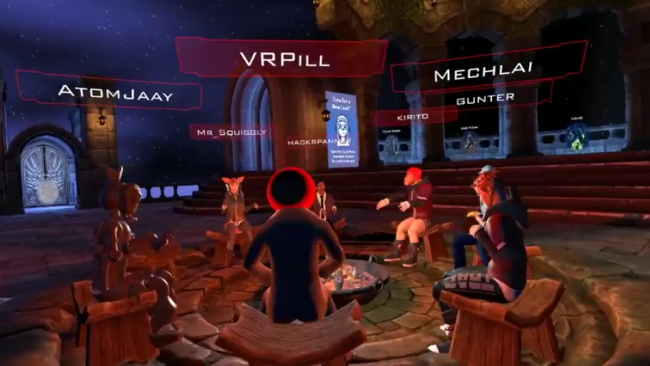
\includegraphics[width=0.5\textwidth]{images/vr_chat.png}
  \caption{In der Anwendung VR Chat können sich meherere Nutzer zum sozialen Austausch treffen. Da diese allerdings individuell navigieren, gibt es bisher keine Technik zur gemeinsamen Navigation}
  \label{fig:todo}
\end{figure}


Mit dem Verkaufsstart von Virtual Reality Headsets wie der HTC Vive oder der Oculus Rift kamen eine Vielzahl von Anwendungen und Spielen auf den Markt, von denen jedoch die überwiegende Anzahl auf einen einzelnen Nutzer ausgerichtet ist. Ausnahmen bilden dabei zwar beispielsweise Apps wie VRChat\footnote{https://www.vrchat.net/}, in denen sich zahlreiche Nutzer treffen und in sozialen Austausch kommen können, dennoch war die Entwicklung bisher primär damit beschäftigt, die Möglichkeiten und Herausforderungen die diese neuartigen Systeme schon bei einem Nutzer mitbringen, auszuloten. 
Denn Anwendungen, in denen mehrere Nutzer gemeinsam interagieren können, bringen eine Vielzahl an größeren Herausforderungen mit sich: Da sich die Nutzer stets in einem getrackten Bereich aufhalten müssen, ist es schwierig eine Lösung zu finden, wie dies für mehrere Nutzer möglich ist, wenn sie VR gemeinsam erleben und sich dabei nicht in die Quere kommen wollen. Ob sich die Nutzer dabei im gleichen realen Raum befinden, oder in unterschiedlichen Räumen mit dem Internet verbunden und dabei die getrackten Gebiete in der virtuellen Realität dann gleich ausgerichtet ("\textit{aligned}") oder unabhängig voneinander sind sind nur die ersten Fragen, die in diesem Kontext aufkommen und ebenfalls aktuell an unserem Lehrstuhl untersucht werden \cite{WeisskerMulti-RayReality}.

Dabei bietet kollaborative VR ein riesiges Potential, wie bereits im einführenden Kapitel erwähnt. Gemeinsam Architekturen zu inspizieren, Datensätze zu explorieren oder Designs und Kunst zu kritisieren sind Beispiele für die bereits jetzt virtuelle Realität an der Bauhaus Universität genutzt wird. Dafür bietet unser Virtual Reality Lab neben Head Mounted Displays mehrere Multi-User Leinwände, an denen bis zu sechs Personen gemeinsam eine teil-immersive virtuelle Realität bereisen können\cite{Kulik2011C1x6}. Diese bringen den Vorteil, dass die Nutzer sich in realer Form sehen können und gleichzeitig mit der virtuellen Umgebung interagieren können, wobei sie in natürlicher Form kommunizieren können.
Arbeiten zur Telepräsenz\cite{BeckImmersiveTelepresence} zeigen, dass man auch entfernte Nutzer über das Internet zuschalten kann und somit mehrere Nutzergruppen verbinden und mit lebensechten Avataren repräsentieren kann. 
Gerade im Hinblick auf die aktuellen Entwicklungen des Weltklimas und dem Anteil, den nicht zuletzt geschäftliche Flugreisen dazu beitragen, können gut nutzbare, kollaborative virtuelle Realitäten dazu beitragen, den Kerosinverbrauch zu minimieren, indem sich Geschäftspartner in solchen Umgebungen "von Angesicht zu Angesicht" treffen können.
Doch bei allen Systemen, egal ob halb oder voll immersiv, ob der Gegenüber real oder ein Avatar ist, bleibt das Problem, dass sich alle Nutzer in einem realen Raum mit realen Abmessungen befinden und sich somit zu Fuß nicht aus diesem bewegen kann. Da für dieses Problem derzeit keine Lösung absehbar ist und es generell bessere Herangehensweisen gibt, als mehrere Kilometer zu Fuß zu laufen, galt und gilt es nun Navigationstechniken zu entwickeln, mit denen man die Grenzen dieses realen Raumes überwindet.

\begin{figure}[H]
	\centering
		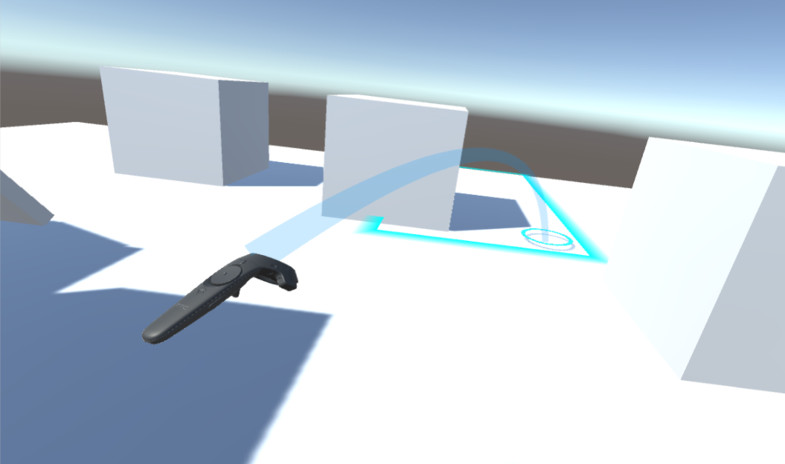
\includegraphics[width=0.8\textwidth]{images/steam_teleport.jpg}
	\caption{Für die Einzelnutzernavigation hat sich \textit{Targed-based Travel} in Form von Teleportation durchgesetzt, der im Bild sichtbar ist. Dabei bekommt der Nutzer seine künftige Position im Raum angezeigt, sowie die Grenzen seine Trackingspaces.}
\end{figure}


Während sich für kleine Distanzen und einem Nutzer der Teleport durchgesetzt hat, bei dem der Nutzer mit seinem Controller das Ziel am Ende eines Bogens auswählt (vgl. Abbildung 2.3), steigen mit zunehmender Nutzerzahl und Distanz die Möglichkeiten zur Umsetzung.
Im Falle unserer Mehrbenutzer Leinwand war das gängige Mittel die Steuerung mittels des sogenannten \textit{Spherons} bei denen ein Steuermann die Nutzergruppe durch die Umgebung \glqq fährt\grqq{}.
Diese Technik bringt allerdings drei Nachteile mit sich. Erstens ist der Großteil der Gruppe bei der Navigation außen vor und hat als Passagier nur eingeschränktes Mitbestimmungsrecht. Dies und die damit verbundene Bewegungsparallaxe schaffen zweitens bei vielen Nutzern ein Gefühl des Unwohlseins, vor allem, wenn zur Translation im Raum auch noch eine Rotation dazukommt. Drittens eignet sich diese Vorgehensweise vor allem für kurze Distanzen und kann über größere Strecken unnötig lange dauern.
Genau an diesem Punkt soll diese Arbeit ansetzen und eine Technik finden, die die bestehende für unser Leinwandsystem ergänzt. Im Ausblick auf zukünftige Fortentwicklungen soll außerdem beschrieben werden, wie diese Technik gegebenenfalls in anderen aktuellen Systemen genutzt werden kann.

\chapter{Qualitätsmerkmale einer Navigationstechnik}
Um eine geeignete Technik zu finden, mit der sich mehrere Nutzer gemeinsam fortbewegen können, bedarf es vorher festgelegter Metriken mit denen sich eine Technik als gut oder nicht gut, geeignet oder ungeeignet klassifizieren lässt.
Bowman et al. \cite{Bowman1998AEnvironments} liefern hierfür eine Liste an Performanz Metriken, die eben dieses leistet:

\begin{addmargin}[25pt]{0pt} 
\textbf{Speed / Task Completion Time}: (Geschwindigkeit / Bearbeitungszeit)\\
\textbf{Accuracy} (Genauigkeit) \\
\textbf{Spatial Awareness} (Raumwahrnehmung) \\
\textbf{Ease of Learning} (Lernbarkeit) \\
\textbf{Ease of Use} (Nutzbarkeit) \\
\textbf{Information Gathering} (Sammeln von Informationen) \\
\textbf{Presence} (Präsenz) \\
\textbf{User Comfort} (Nutzerkomfort) \\
\end{addmargin}
 
Ein beispielhafter Use Case kann helfen, diese Metriken in unserem Kontext zu verstehen:
Man stelle sich vor, eine Nutzergruppe (wie beispielsweise die Tourismusgruppe aus dem einleitenden Beispiel) stände in einer virtuellen Umgebung vor einem Monument, zum Beispiel dem Haupthaus der Bauhaus Universität in Weimar, und will infolgedessen zu einem anderen Platz gelangen, welcher sich nicht in der Nähe befindet. Ein (eher nahegelegenes) Ziel wäre z.B. das Denkmal von Goethe und Schiller vor dem deutschen Nationaltheater in Weimar oder der (sehr viel entferntere) Fernsehturm in Berlin
Die Zeit vom Beginn der Reise, über das Auswählen des Ziels, sowie der Reise und dem Ankommen am Ziel sind dabei im erste Kriterium \textbf{(1: Task Completion Time)} repräsentiert.\\
Die Präzision \textbf{(2: Accuracy)} beschreibt dabei, wie exakt die Reisegruppe am gewünschten Ziel ankommt. Das heißt, ob die \glqq Touristen\grqq{} nach der Reise genau vor dem Fernsehturm steht oder nur nahegelegen im Berliner Zentrum. Ist die Technik dagegen sehr präzise, kann die Reisegruppe entscheiden, wo genau sie vor oder in dem Fernsehturm steht. Dies würde aber zumeist bedeuten, dass sie aufwändiger zu benutzen ist \textbf{(5: Ease of Use)}, da eine so exakt geplante Reise viel aufwändiger durchzuführen ist, als eine grobe Zielauswahl.\\
Für die Nutzbarkeit spielt aber auch das Interaktionsdesign der entsprechenden Technik eine wichtige Rolle, welches, wenn einfach gestaltet, die Technik leichter zu benutzen macht. Im besten Fall gilt dies auch für Einsteiger, sodass auch ungeübte Nutzer schnell eine entsprechende Navigationsabfolge planen und durchführen können \textbf{(4: Ease of Learning)}.\\
Das Kriterium des Sammelns von Informationen während der Reise (\textbf{6: Information Gathering)} würde in unserem Kontext beschreiben, wie viel der Nutzer während der Reise gelernt hat. Solche Informationen wären z.B. der genaue Weg vom Bauhaus zum Theater oder die genutzten Autobahnen und deren angrenzenden Großstädte auf dem Weg nach Berlin.\\
Das Kriterium der räumlichen Wahrnehmung \textbf{(3: Spatial Awareness)} wiederum bestimmt, wie gut Nutzer ihre aktuelle Position im Raum nach der Reise einschätzen können. Wissen die Nutzer, in welche Richtung sie nach des Reise sehen, wo sie sich auf dem Globus befinden und aus welcher Himmelsrichtung sie gekommen sind?\\
Die Präsenz \textbf{(7: Presence)} beschreibt dabei das Gefühl der Immersivität der Reise, also das Gefühl, dass die virtuelle Umgebung den Nutzern real erscheint. Wird während der Reise, durch Aufgaben oder Abläufe die Konsistenz der virtuellen Umgebung gebrochen, wird diese Metrik verletzt.\\
Der letzte Punkt beschreibt, wie gut sich die Technik auf das Wohlbefinden des Nutzers \textbf{(8: User Comfort)} auswirkt. Hierbei sollte sichergestellt werden, dass es keinem Nutzer durch das Nutzen der Reisetechnik schwindelig oder übel wird, denn in vielen Fällen bringt die Fortbewegung in virtuellen Umgebungen ein Unwohlsein mit sich.

Da ein Schwerpunkt dieser Arbeit jedoch auf dem Reisen als Gruppe liegt, bedarf es eines weiteren Kriteriums, welches Bowman et al. im Hinblick auf Einzelnutzernavigation nicht berücksichtigten, nämlich den Aspekt der Gruppeninteraktion \textbf{(9: Cooperation)}. Wie gut die Gruppen interagieren kann, ob jeder involviert wird und für alle die schon genannten Kriterien gleichermaßen gelten, sind Aspekte, die in diesem Punkt zu berücksichtigen sind.
So wäre das gemeinsame Einverständnis zum \glqq Antritt\grqq{} sowie das gemeinsame Planen der Reise, Punkte deren Nutzbarkeit im Gruppengefüge untersucht werden müssen.

Auf all diese Kriterien soll auch bei der Entwicklung unserer Technik eingegangen werden. Wie genau sie in verwandten Arbeiten gemessen werden und in welcher Form diese Quantisierung in unserem Fall stattfindet, wird in der Beschreibung einer möglichen Studiendurchführung im 9. Kapitel näher beschrieben.

\chapter{Navigationstechniken in VR}
\begin{figure}[h!]
  \centering
  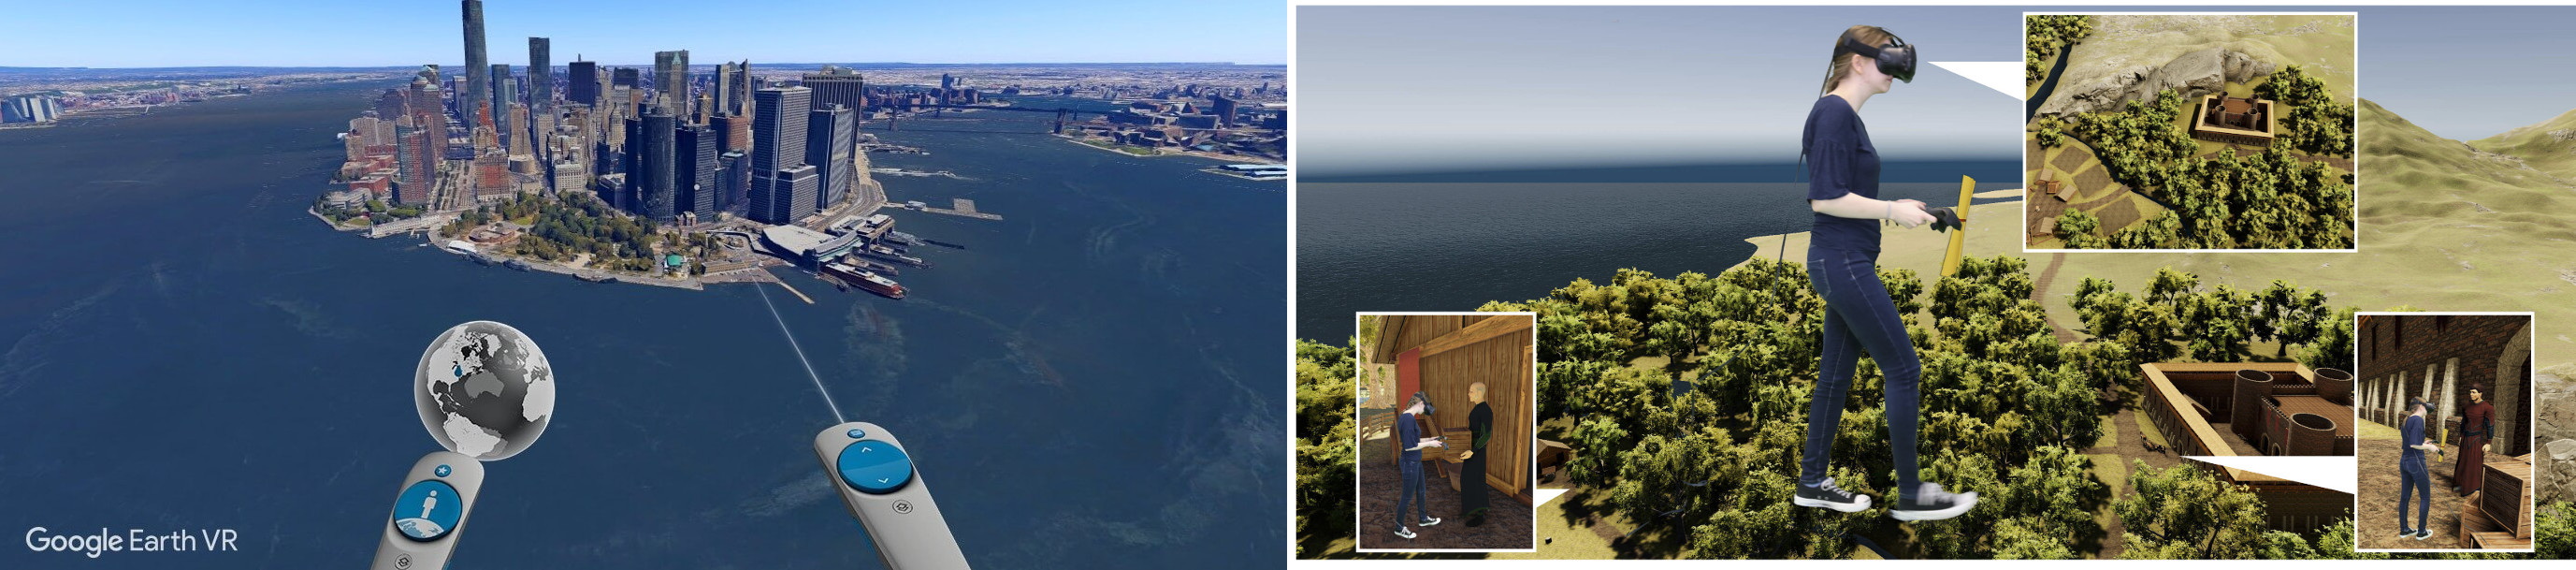
\includegraphics[width=\textwidth]{images/google_gulli.jpg}
  \caption{Google Earth VR (links) vereinigt \textit{Physical Movement}, \textit{Steering}, \textit{Manual Viewpoint Manipulation} und \textit{Physical Movement}, während GulliVR\cite{Krekhov2018GulliVR} dem Nutzer auf Riesengröße wachsen lässt, um große Distanzen zu überwinden}
  \label{fig:todo}
\end{figure}

In den letzten Jahren wurden zahlreiche Arbeiten zum Reisen in virtuellen Umgebungen entwickelt und veröffentlicht, die sich (zumeist) an den im letzten Kapitel beschriebenen Kriterien orientierten, wobei aber die Gewichtung dieser Qualtitätsmerkmale sehr varrierte, denn die zu bereisenden virtuellen Realitäten können verschiedenster Natur sein. Daher unterscheiden sich die Techniken zur Navigation anhand ihrer Motivation, der genutzten Hardware, der Nutzerzahl, aber nicht zuletzt auch der Umgebung.
In der akademischen Forschung sind die Umgebungen, für die eine entsprechende Navigation entwickelt werden, vielfältig.
Zum einen werden Techniken entwickelt, die sich primär für den Gebrauch im Freien eignen. Beispiele hierfür sind das Reisen zwischen mittelalterlichen Dörfern \cite{Krekhov2018GulliVR} oder in größerem Umfang die Navigation in hierarchisch strukturierten Umgebungen, bei denen der Nutzer wie bei Google Earth fließend zwischen Nachbarschaften, Städten, Ländern oder Kontinenten wechselt \cite{pierce_representations}.
Außerdem werden neben dem Manövrieren innerhalb von Gebäuden, wie Einkaufszentren oder einzelnen Stockwerken (z.B. \cite{Richardson1999SpatialEnvironments}, \cite{Liang2018EvaluatingEnvironments}) selbstverständlich auch Szenarien untersucht, bei denen es gilt sowohl Indoor als auch Outdoor zu navigieren, beispielsweise durch Haus und Terrasse einer Villa wie bei \cite{Dallat2018Giant}. 
Virtuelle Realitäten bieten aber auch die Möglichkeit sich durch Datensätze wie zum Beispiel der Visualisierung einer Punktwolke oder sich durch den menschlichen Körper \cite{Kopper2006DesignEnvironments} zu navigieren.

Durch die Möglichkeit beinahe alle vorstellbaren Szenarien in einer immersiven Umgebung darstellen zu können, sind die einhergehenden Motivationen zur Navigation vielfältig. Dennoch lassen sie sich in drei grundlegenden Typen klassifizieren: \textbf{Exploration}, \textbf{Search} und \textbf{Maneuvering} (\cite{Bowman2001AnDesign}, \cite{KulikBuildingTechniques}). 
Diese Einteilung lässt sich sowohl für Einzel- und Mehrbenutzernavigation, als auch für die Navigation auf gleichbleibenden oder unterschiedlichen Skalierungen vornehmen.
Exploration beschreibt dabei einen freien Navigationsvorgang, wie das Spazieren durch eine unbekannte Stadt. Dabei wird während des Bewegens die Umgebung erkundet, indem man sich umsieht, also eine Rotation des Standpunktes vornimmt. 
Dies kann man allerdings auch auf eine andere Skalierungsebene übertragen. Das entsprechende Beispiel wäre das freie Erkunden des Stadtplans, in dem man ohne sich eines Ziels bewusst zu sein, den Aufbau der Stadt ergründet. Klassischerweise tut man das in dem man die Lage wichtiger Punkte (z.B. Bahnhof, Stadtzentrum, Denkmäler etc.) zueinander betrachtet und mögliche Routen frei “inspiziert”.\\
Die Suche beschreibt dagegen den Vorgang des Findens des effizientesten Weges von einem Start A zu einem Ziel B. Auch hier lässt sich wieder das Navigieren in einer fremden Stadt als Beispiel nehmen. Befindet man in der “realen Skalierung” eines Touristen wäre die Orientierung an Wegweisern und Straßenschildern der Weg um die kürzeste Route von dem aktuellen Standpunkt zu einer Touristenattraktion. Hier kommt jedoch zumeist der Stadtplan ins Spiel, bei dem der Tourist eine bessere Übersicht hat und somit den effizienteren Weg schnell finden kann.\\
Während der Vorgang des Gehens in diesen Beispielen dem nach Bowman beschriebenen ”\textit{Travel}”-Prinzips entspricht, also der tatsächlichen Reise, während der Blick auf die Karte dem ”\textit{Wayfinding}” zuzuordnen ist. 
Im besten Fall kann eine Navigationstechnik all diese Ansprüche bedienen: Er kann sie nutzen, um den Weg zu finden und diesen schnell zu beschreiten, unabhängig ob er sein Ziel kennt oder einfach nur die ganze Umgebung ausgiebig erkunden will.

Das Manövrieren stellt eher das Verändern des Sichtpunkts um ein Objekt herum da, um es in verschiedenen Orientierungen zu betrachten oder um besser mit diesem interagieren zu können. Diese ist sehr viel feingliedriger und könnte im Beispiel des Touristen ein Umkreisen eines Denkmals sein, was dieser genauer betrachten will. Dieser Vorgang findet in den meisten Fällen (wie z.B. in unserer Multiuser Leinwand) durch das Bewegen des eigenen Körpers und des Kopfes statt und ist in diesem Fall kein Bestandteil einer Navigationstechnik.

Doch während beim Entwickeln einer neuen Technik die zu bereisende Umgebung und die Motivation, weshalb gereist wird, sicherlich wichtige Faktoren sind, stellt der wichtigste Gesichtspunkt die Art und Weise dar, in welcher navigiert wird. Bowman et al. \cite{Bowman2001AnDesign} unterteilen hierbei Navigation in 5 Metaphern: \textbf{Physical Movement}, \textbf{Manual Viewpoint Manipulation}, \textbf{Steering}, \textbf{Target-based Travel} und \textbf{Route Planning}. 
\textit{Physical Movement} beschreibt dabei, dass sich der oder die Nutzer in der realen Umgebung mit ihren (realen) Körpern bewegen. Dies kennt man von trackingbasierten Systemen wie der HTC Vive, bei denen sich der Nutzer mit seinem getrackten Headset in einem realen Umfeld bewegt und seine Bewegung in die virtuelle Umgebung, die dieser in diesem Moment sieht, umgesetzt wird.
Bei der \textit{Manual Viewpoint Manipulation} kann der Nutzer sich in der Welt ”entlanghangeln”. Dies geschieht, in dem er sich virtuellen Gegenständen oder ggf. in der Luft “festhält” und die virtuelle Welt zu sich “heranzieht”. 
In dreidimensionalen Computerspielen, wie z.B. Ego-Shootern oder Flugsimulatoren, findet man die vermutlich bekannteste Fortbewegungsweise, das \textit{Steering}. Hierbei kontrolliert der Nutzer zu jedem Zeitpunkt seine Translation und Rotation im Raum.
Gerade seit dem Aufkommen konsumentenfreundlicher Systeme der virtuellen Realität wird die Nutzung von \textit{Targed-based Travel} populärer: Hierbei spezifiziert der Nutzer sein Reiseziel und das System übernimmt die Transition zu diesem. 
Google Earth VR vereinigt dabei alle Metaphern bis auf \textit{Route Planning}. Durch das Anzeigen der Richtung mit dem Controller und gleichzeitigem Knopfdrücken kann man durch die Welt fliegen (\textit{Steering}). Alternativ kann man auch einen Punkt in der Welt greifen und zu sich heranziehen (\textit{Manual Viewpoint Manipulation}). Um einen \textit{Target-based Travel} einzuleiten, kann man auf der Weltkugel (vgl. Abbildung 8.1), welche man in der linken Hand hat, einen Punkt in der Welt selektieren und wird zu diesem teleportiert. Gleichzeitig ist es zu jedem Zeitpunkt möglich seine aktuelle Position durch Laufen im eigenen Trackingspace zu verändern (\textit{Physical Movement}) 

Ein bekanntes Beispiel dafür ist die in VR oft genutzte Teleportation, mit der der Nutzer sich über die Grenzen des Bereichs, den er durch physische Bewegung erreichen kann, hinfort bewegt (vgl. Abbildung 2.3).
Das \textit{Route Planning} stellt zu guter Letzt eine Technik da, mit der der Nutzer einen Weg spezifiziert, auf welchen ihn das System daraufhin bewegt. Dies erlaubt dem Nutzer während der Bewegung andere Aufgaben auszuführen und sich nicht ausschließlich auf die Reise zu konzentrieren. Die verwandten Arbeiten die im Folgenden vorgestellt werden, beziehen sich auf die Themen Gruppennavigation und Navigation über große Distanzen und nutzen diese Metaphern. Allerdings kann bereits an dieser Stelle verraten werden, dass \textit{Manual Viewpoint Manipulation} besonders aber \textit{Route Planning} nicht auftauchen, da sie nicht zu den populärsten Metaphern zählen.

\section{Navigation in Gruppen}
Bisher gibt es sehr wenige Arbeiten, die sich mit dem Thema der Gruppennavigation in virtuellen Umgebungen beschäftigen. Eine dieser Arbeiten, welche inhaltlich nahe am Thema dieser Arbeit ist, ist die Arbeit von Weißker et al. (\cite{WeisskerMulti-RayReality}). Darin wird eine neue Technik vorgestellt, die sich mit dem gemeinsamen Teleport von zwei Personen beschäftigt. Auch hier wird als beispielhaftes Szenario der Stadtführer, welcher einen zweiten Nutzer (passiver Nutzer, Passagier) durch eine Stadt führt, genannt. 
In diesem Fall spielt sich die Navigation allerdings im Vista-Raum ab und wird auf Head Mounted Display getestet. Sie stellt eine Erweiterung der oben genannten Teleporttechnik dar, wobei der passive Nutzer vom Führenden auf verschiedene Arten mitgenommen wird (\textit{Coupled, Vehicle und Congruent}. Die Technik in unserer Arbeit kann als Ergänzung zu dieser Arbeit gesehen werden. Dabei dient erstere für den Sprung über große Distanzen, letztere dann für kleinere Distanzen innerhalb des sichtbaren Bereichs. Einige Erkenntnisse gelten dabei für beide Distanzen: Zum einen ist es immens wichtig, dass der Navigator zu jedem Zeitpunkt die aktuellen Positionen seiner Mitreisenden kennt und auch weiß, wo diese Position nach dem Teleport sein werden um Kollision zu vermeiden und sicherzustellen, dass entsprechende POIs im Blickfeld von allen liegen. Dies gilt im Übrigen auch für die anderen Nutzer, damit sie sich auf die Konsequenzen des Sprungs einstellen können. Dieses wird dadurch ermöglicht, dass auch der passive Nutzer einen Strahl zu seinem voraussichtlichen Teleport Ziel angezeigt bekommt. Dies minimiert Fehler in der Platzierung durch den aktiven Nutzer und reduziert die kognitive Last beider Nutzer, führt allerdings zu einem etwas längeren Planungsvorgang vor der Reise. Weiterhin stellen die Autoren fest, dass das Wohlbefinden bzw. die Simulatorenkrankheit des passiven Nutzers nicht deutlich stärker ist, als bei einem Einzelnutzer Teleport. Verbunden mit der nötigen Aufmerksamkeit des aktiven Nutzers und einer effektiven Kommunikation wird somit eine erfolgreiche Navigation ermöglicht, sodass der passive Nutzer bei dieser nicht mit der Umgebung kollidiert. Dies stellt nämlich eine der größten Schwierigkeiten der gemeinsamen Navigation dar, womit sich Kulik et al. (\cite{Kulik2011C1x6}) beschäftigen. Diese befassen sich neben der Hardware unseres Lehrstuhls deren Weiterentwicklung acht Jahre später in dieser Arbeit genutzt wird mit dem Problem, dass nicht immer alle Gruppenmitglieder in einem gemeinsamen Tracking Space in den möglicherweise viel kleineren, virtuellen Raum passen. In diesem Fall wird allerdings die \textit{Steering} Navigation genutzt, von der sich jetzt schon abzeichnet, dass sie aufgrund der Dauer und des Motionflows für größere Distanzen weniger geeignet ist, als ein Teleportationsvorgang.
Ein weiterer Hinweis auf die Navigation mit mehreren Nutzern findet sich in der Arbeit von Beck et al.(\cite{BeckImmersiveTelepresence}). Hier bewegen sich zwei Gruppen gemeinsam in einer virtuellen Welt, wobei ihnen die Möglichkeit gegeben wird, sich unabhängig voneinander zu bewegen oder dem anderen Team zu folgen. Der besondere Aspekt dabei ist aber, dass sich die Nutzer in einer World in Miniature (siehe übernächster Absatz) sehen können und das andere Team in dieser selektieren und an einen anderen Ort bewegen können. Obwohl selbst die Autoren zugeben, dass diese Methode bei den Mitgliedern des Teams, welches versetzt wird, Unwohlsein auslöst, ist die Idee, eine WIM zur Navigation zu nutzen, indem man die Plattform der Nutzer in dieser platziert eine spannende und vielversprechende Vorgehensweise, auf die im übernächsten Absatz genauer eingegangen werden soll. 



\section{Skalierungsbasierte Techniken}
Viele Anwendungen und Programme bieten neben den allgemein genutzten sechs Freiheitsgraden, drei für Translation und drei für Rotation noch einen weiteren Freiheitsgrad:
Die fünf bekannten Metaphern (\textit{Steering} usw.) werden erweitert durch die Modifizierung der Größe des Nutzers in der virtuellen Umgebung. Dies hat zwei entscheidende Vorteile. Zum einen kann der Nutzer seine Umgebungen in verschiedenen Skalierungen betrachten. Ein Nutzer, der die Größe eines Riesen hat, kann eine Region weitaus besser Überblicken, während er in der Größe von wenigen Zenti- oder gar Millimetern kleinteilige Regionen einer Umgebung explorieren kann. Doch neben dem visuellen Vorteil bietet die Modifizierung der eigenen Größe einen für diese Arbeit viel wichtigeren Vorteil. In der Größe eines Riesen kann der Nutzer bei gleichbleibender wahrgenommener Geschwindigkeit viel größere Distanzen überwinden als in seiner normalen Größe mit normaler Laufgeschwindigkeit.
Dies machen sich zum Beispiel Krekhov et al. (\cite{Krekhov2018GulliVR}) in ihrer Arbeit zu nutze. Nach dem \textit{Physical Locomotion} Prinzip kann sich der Nutzer in einem realen Raum bewegen und dabei zwischen dem sogenannten \textit{Normal Mode} und \textit{Giant Mode} wechseln. Zweiteres bedeutet, dass der Nutzer auf die Größe eines “Giganten” vergrößert wird. Die Zielgröße wird dabei so festgelegt, dass der Nutzer das weiter entfernte Dorf, welches er zur Erfüllung seiner Aufgabe aufsuchen muss, erreichen kann, in dem er mit wenigen Schritten innerhalb seines realen Tracking Spaces zu diesem Dorf läuft, um sich dort wieder zu schrumpfen. In diesem \textit{Giant Mode} wird der Augenabstand so modifiziert, dass der Nutzer das Gefühl hat in einer Miniaturwelt zu stehen, anstatt über der Welt zu fliegen. Will der Nutzer sich wieder auf seine Ausgangsgröße zurück schrumpfen, bieten die Verfasser zwei Methoden: Beim \textit{Targeting} wird dem Nutzer mit einem Zielkreuz zu seinen Füßen angezeigt, wo er nach der Skalierung stehen wird, beim \textit{Pulling} wird der Nutzer, wenn er sich innerhalb eines festgelegten Areals befindet, während er geschrumpft wird zu einem vorher definierten Point of Interest bewegt, sodass er nach der Transition direkt vor diesem steht. (vgl. Abbildung)
Die drei Hypothesen, dass der Nutzer a) ein erhöhtes Präsenz-/ Überblicksgefühl hat, b) keine Cybersickness empfindet und c) signifikant mehr läuft, konnten in einer Vergleichsstudie, in der gegen die Fortbewegung durch das aus SteamVR bekannte Teleportieren getestet wurde, bestätigt werden.
Diese Ergebnisse lassen sich allerdings nur bedingt auf die Entwicklung einer Technik für mehrere Nutzer im kohärenten Workspace übertragen, da ein gemeinsames Laufen in einer Gruppe ein Problem darstellt. So müssten alle Nutzer gleichzeitig größer bzw. kleiner skaliert werden, damit die Kohärenz des Workspaces nicht aufgehoben wird. Zusätzlich muss dazu noch ein gemeinsames Laufen koordiniert werden, was nicht nur wegen der zumeist geringen Größe des Tracking Spaces ein schwieriges Unterfangen wäre. Denn in Hinblick auf die Nutzung an unserem semi-immersiven Leinwandsystem ist ein solcher gemeinsamer Spaziergang ausgeschlossen. Ansätze, wie sich der vorhandene Tracking Space wie z.B. durch ”\textit{Redirected Walking}” (\cite{RazzaqueRedirectedWalking}) besser nutzen lassen könnte, sind für mehrere Nutzer in gemeinsamen Workspaces und vorallem am Leinwandsystem ebenfalls keine Alternative. 
Dennoch lassen sich die Erkenntnisse zur schnelleren Überwindung von Distanzen und des erhöhten Präsenzgefühls durch den Blick von oben nutzen. Denkbar wäre z.B. ein gemeinsames Aufskalieren, mit anschließendem Teleportations- bzw. Steeringvorangs, wobei die wahrgenommene Reisedistanz deutlich abnimmt.

Einen ähnlichen Weg gehen McCrae et al.\cite{McCrae2009MultiscaleNavigation}.
Der Nutzer kann dabei also frei in der Welt umherfliegen, wobei seine Größe und seine Bewegungsgeschwindigkeits stets so modifiziert werden, dass er das Gefühl einer fließenden und gleichbleibenden Fortbewegungsgeschwindigkeit wahrnimmt. 
Die tatsächliche Größe und somit auch Geschwindigkeit, sowie die Anpassung der near- und far-clipping plane werden mit Hilfe einer sogenannten ”\textit{Cube Map}” bestimmt. Dabei wird ausgehend von der aktuellen Kameraposition in alle sechs kanonischen Richtungen ein 64x64 Bit Bild errechnet, welches die Distanzen zu allen Objekten kodiert (vgl. Abbildung). Anhand der minimalen Distanz dieser ”\textit{Cube Map}” werden die resultierenden Skalierungsparameter errechnet.
Das Resultat ist, dass Nutzer durch die Umgebung fliegen können ohne selbst manuelle Einstellungen der Skalierungsparameter ausführen zu müssen. Diese Vorgehensweise wird von Argelaguet et al. \cite{Dallat2018Giant} weiter verbessert, um Nutzern ein noch besseres Gefühl von konstanter Bewegungsgeschwindigkeit bei unterschiedlichen Skalierungen erhalten.
Kopper et al. \cite{Kopper2006DesignEnvironments} verfolgen den Ansatz, die Parameter entsprechend des jeweiligen Gebiets, in dem sich der Nutzer befindet, anzupassen. In ihrem Anwendungsfall wird der menschliche Körper und dessen Organe bereist. Die Auswahl der Parameter wird entsprechend des Volumens der \textit{Bounding Box} des Organs, in welchem man sich befindet, gewählt. Dabei bieten die Verfasser zwei Möglichkeiten zur Navigation: Zum einen können Nutzer wie in den zuvor genannten Arbeiten durch \textit{Steering} durch den Körper “fliegen”. Stoppen die Nutzer in einem Organ, so wird Augenabstand, Fluggeschwindigkeit und somit die wahrgenommene Körpergröße je nach vorherigen Parametern entweder verkleinert oder vergrößert. In der zweiten Möglichkeit, kann der Nutzer mit Hilfe einer Lupen Metapher Organe auswählen und wird dann automatisch in deren Zentrum gesetzt, wobei auch hier die Anpassung der Parameter stattfindet.
Der Ansatz der automatischen Anpassung der Navigations- und Stereoparametern wird so oder in abgewandelter Form auch bei Google Earth VR genutzt. Diese Technik kann und wird auch in Mehrbenutzerszenarien benutzt, jedoch benötigen \textit{Steering}-Techniken immer einen Steuermann. Dies wiederum bedeutet immer, dass es passive Nutzer gibt, die nicht an der Navigation und somit der Zielfindung beteiligt sind. Außerdem kommt es bei \textit{Steering}-Techniken in virtuellen Realitäten häufig zur \textit{Simulator Sickness} (vgl. \cite{Lackner2014MotionVomiting}).
Ein \textit{Targed-based}-Vorgehen wie in der zweiten Variante Koppers wäre für mehrere Anwender sicher besser geeignet, da sich hierbei die Nutzer vor der Reise über das Ziel einig werden können und gegebenenfalls auch so geplant werden kann, dass sich nach der Transition wirklich alle Nutzer innerhalb des gewünschten Organs bzw. allgemein Zielgebiets befinden können.

Generell lässt sich sagen, dass skalierungsbasierte Techniken einen guten Ansatz bieten, die bekannten Bewegungsmetaphern auf große Distanzen zu erweitern, dennoch lassen sich zahlreiche Kriterien aus Kapitel 2 mit den bisherigen Ansätzen nicht erfüllen:
\textit{Steering} und \textit{Physical Walking} wirken sich negativ auf die Bearbeitungszeit aus, der Nutzerkomfort für passive Nutzer wird ebenfalls eingeschränkt und auf das Prinzip der Gruppeninteraktion wird in keinem Ansatz eingegangen.

\section{Navigation mit Hilfe von World in Miniatures}

Ein weiterer Ansatz zur Navigation in virtuellen Umgebungen wurde bereits 1970 von Stoakley et al. \cite{Stoakley2010VirtualWIM} vorgestellt. Das Konzept der sogenannten \textit{World in Miniature} (im folgenden: WIM) beschreibt eine miniaturisierte Kopie der Umgebung bzw. Welt in der sich der Nutzer gerade befindet. Mit dieser Metapher ist es dem Nutzer nicht nur möglich einen exozentrischen Blick von oben auf die ihn umgebende Hauptszene zu werfen, sondern er kann diese Miniatur auch als Interface nutzen. Die Möglichkeiten dieses Interface sind dabei vielfältig. Genau wie in der Hauptszene bietet sie drei Möglichkeiten zur Interaktion: Selektion, Manipulation und Navigation.
Selektion und Manipulation bedeutet in diesem Zusammenhang, dass der Nutzer in die WIM “greifen” kann und dabei z.B. die Position und Ausrichtung eines Objektes verändern kann, wobei die Änderungen in der Miniaturwelt zeitgleich in der Hauptszene umgesetzt werden. Die Vorteile einer solchen Manipulation liegen (wortwörtlich) auf der Hand: Der Nutzer muss nicht mehr in der Hauptszene zu Objekten navigieren, sondern kann diese einfach in der WIM zu sich ziehen. 
Weiterhin besteht aber auch die Möglichkeit, dass der Nutzer die Repräsentation seiner selbst auswählt, um diese (und somit sich selbst) zum entsprechenden Objekt zu manövrieren. So wird die Metapher der Manipulation zur Navigationsmetapher.
Diese Metapher bedurfte allerdings weiterer Optimierung. Setzt man nämlich den Positionswechsel des Nutzers zeitgleich in der egozentrischen Sicht um, kann dies zu starker Desorientierung führen. In ihrer ursprünglichen Arbeit schlagen die Verfasser zwei Alternativen vor: Entweder wird der Navigationsvorgang erst nach dem Abschluss der Manipulation durchgeführt, in dem der Nutzer in seiner egozentrischen Sicht mit einem flüssigen Übergang an sein gewähltes Ziel animiert wird oder der Nutzer kann mehrere Manipulationen durchführen, welche erst zum Zeitpunkt eines Knopfdrucks umgesetzt werden (”\textit{batching}”). 
Diese beiden Vorschläge wurden von Stoakleys Kollegen Pausch et al. (\cite{5_pausch_WIM}) durch eine Option erweitert, in welcher der Nutzer, nachdem er seine Repräsentation platziert hat nicht in der Welt in Originalgröße zu diesem Ort animiert wird, sondern direkt in seine eigene Repräsentation in der WIM hinein, sodass er sich danach auch in dieser befindet.
Das hat den den entscheidenden Vorteil, dass der Nutzer seine Aufmerksamkeit nicht erst wieder auf die ihn umgebende Welt richten muss, sondern die Navigation in seinem aktuellen kognitiven Fokus stattfindet, was Verwirrung und Desorientierung mindert. In diesem Fall wird die vormals exozentrische zur egozentrischen Ansicht.
Die Autoren geben allerdings zu Bedenken, dass bei diesem ”Zoom-In” Vorgang Kollisionen mit der Umgebung stattfinden können, welche durch vorherige Routenplanung ausgeschlossen werden müssten und dass die zurück zu legenden Distanzen die bei dieser Transition sehr groß sein können. 
Neben dem - in dieser Technik vorhandenen - Motionflow, der bei der Entwicklung unserer Technik ausgeschlossen werden soll, um Unwohlsein zu minimieren, spricht besonders der erste der genannten Aspekte gegen eine Nutzung dieser Technik für mehrere Nutzer. Denn während sich bei einer Gruppe von Nutzern eine solche Transition wegen der verschiedenen Standpunkte sowieso schon schwerer gestaltet, muss zusätzlich Rücksicht auf eventuelle Kollisionen genommen werden.

Eine weitere Möglichkeit, eine WIM zur Navigation zu benutzen, wurde im Anschluss auf die Arbeit von Staokley von LaViola et al. (\cite{LaViola2004Hands-freeEnvironments}) in Form der sogenannten  ”\textit{Step WIM}”  vorgestellt.
Eine zentrale Motivation dieser Arbeit war, die WIM - anders als bei Stoakley - nicht in der Hand halten zu müssen und die Hände somit für andere Aktivitäten nutzen zu können. 
Um dieses Kriterium einzuhalten wird die WIM auf den Boden, der sich im Zentrum von drei würfelförmig angeordneten 3D Leinwänden befindet, projiziert (vgl. Abbildung). Das hat weiterhin zum Vorteil, dass die WIM nicht mehr im Sichtfeld ist und somit keine wichtigen Teile der Szene verdeckt. 
Um eine Interaktion mit der Projektion zu ermöglichen, entwickeln die Autoren eine Vielzahl an Techniken, in denen unter anderem das Tracking der Hüfte sowie sogenannte ”\textit{Interaction Slippers}”, also Schuhe, welche als Eingabegerät dienen, genutzt werden.
So kann der Nutzer innerhalb der WIM zum gewünschten Ziel laufen und ohne die Nutzung seiner Hände den Befehl geben, dass die WIM an der Stelle an welcher er sich befindet hochskaliert wird, sodass der Nutzer sich an tatsächlich an der gewünschten Stelle befindet.
Auch kann der Nutzer die WIM durch Laufen skalieren. Die vorgestellten Interaktionstechniken bringen allerdings einen nicht zu unterschätzenden kognitiven Aufwand mit sich. 
Um die Navigation einzuleiten muss der Nutzer z.B. seine Zehen zusammenführen oder mit der Hüfte eine Hüpfbewegung machen. Der Skalierungsprozess wiederum wird durch das Zusammenführen der Fersen initiiert, woraufhin die WIM durch Laufen skaliert wird und das Zentrum der Skalierung durch die Kopfposition des Nutzers bestimmt wird, bis dieser wieder seine Fersen zusammenführt. Gleichzeitig kann der Nutzer die WIM oder sich selbst in der Welt translatieren, wobei hier die Blickrichtung (in Richtung Boden oder Wand) entscheidet, welche der beiden Funktionen ausgeführt wird.
Auch wenn diese Interaktionen (vor allem das Skalieren der WIM) ein wichtiger Teil des Navigationsprozesses sind, stellt sich die Frage, ob der Interaktionsfluss nicht doch durch die ungewohnte Nutzung der Füße und Hüfte als Eingabegerät eingeschränkt wird.
Im Hinblick auf die Benutzung durch mehrere Nutzer lässt sich sagen, dass durch die gute Sichtbarkeit der Bodenprojektion alle Nutzer eine gute Vorstellung ihrer aktuellen Position und der Interaktion mit der WIM hätten. Eine Umsetzung dieser Technik, bei der ein geübter Navigator eine Personengruppe mit Hilfe der Step WIM durch eine virtuelle Umgebung leitet ist durchaus denkbar. Dabei wäre denkbar die, doch etwas ungewohnten Fußeingaben, durch Eingaben mit einem Eingabegerät in der Hand zu ersetzen. So könnte man bei den Pointern, wie sie in unserem System genutzt werden, durch ihren aktuellen Winkel den Kontext ableiten: Neigt man den Controller soweit nach unten, dass sein Vorwärtsvektor nicht mehr die Leinwand, sondern den Boden schneidet, würde automatisch die Interaktion mit der WIM, statt mit der Szene, aktiviert.

Während LaViola et al. ihre ”\textit{Step WIM}” auf kontinuierliche Weise auf- und wieder abskalieren, um weiter entfernte Regionen zu erreichen, nutzen Pierce et al. \cite{pierce_representations} eine diskrete Anzahl von hierarchisch strukturierten Voransichten. Dabei liegt der Schwerpunkt darauf große, virtuelle Umgebungen sehr schnell zu bereisen.
Mit dem Grundgedanken, dass sich Nutzer vor allem mit Hilfe von visuellen Orientierungspunkten, wie Denkmälern, Sehenswürdigkeiten oder sonstigen eindrücklichen Objekten in einer Umgebung zurechtfinden, stellen die Verfasser dem Nutzer Repräsentationen von Orten zur Verfügung, die er nutzen kann, um an diese Orte zu reisen.
Dabei kann jede Repräsentation als eine Art WIM angesehen werden, wobei diese hierarchische Skalierungslevel der Umgebung darstellen. In der niedrigsten Hierarchiestufe sind diese Repräsentationen tatsächliche Kopien der dargestellten Welt. In allen Stufen darüber zeigen die Repräsentationen vereinfachte Darstellungen des Gebiets, indem nur für die Identifizierung dieses Gebiets wichtige Orientierungspunkte zu sehen sind (vgl. Abbildung).
Die Hierarchien entsprechen dabei den im Alltag benutzten Begriffen “Nachbarschaft”, “Stadtteil”, “Stadt”, “Region”, “Land”, “Bundesland”, und so weiter.
Will der Nutzer nun von einer Stadt in eine andere reisen, z.B. von Lyon nach Paris, kann er sich durch die Hierarchie des Baumes navigieren. Die Repräsentationen des aktuellen Levels, so wie dem Level darüber werden um den Nutzer herum angezeigt. Deutet er auf sie und bestätigt dies mit einem Knopfdruck, wird die gewählte Repräsentation in seine Hand befördert. Handelt es sich um eine vereinfachte Repräsentation, also nicht auf dem niedrigsten Level, kann er aus dieser die gewünschte Repräsentation des nächst- niedrigeren Levels herausziehen. 
Gehört die Repräsentation zum untersten Level (also zur “Nachbarschaft”), kann der Nutzer sie in seiner Hand so positionieren, dass er aus dem gewünschten Blickpunkt in die tatsächliche WIM schaut. Bestätigt er diesen, berechnet das System den korrespondierenden Sichtpunkt in der Hauptszene und der Nutzer wird automatisch an diesen Punkt teleportiert.
Diese Vorgehensweise bietet mehrere Vorteile: Zum einen ist eine schnellere und effizientere Vorgehensweise als die Traversion eines Baumes zum Erreichen entfernter Orte kaum möglich. Zum anderen stellt die finale Positionsauswahl durch Ausrichtung der WIM und Berechnung des korrespondierenden Blickpunkts eine intuitive Möglichkeit zur Zielbestimmung des Teleports. Diese Vorgehensweise kann allerdings schlecht in Mehrbenutzerszenarien angewandt werden, da immer nur eine Person in der Lage ist, den Blickpunkt in der WIM zu bestimmen. Die anderen wissen infolgedessen nicht zwangsläufig, welche Position dieser Nutzer ausgewählt hat.

Ein Lösungsansatz für diese Problematik lässt sich in der Arbeit von Kunert et al. (\cite{Kunert2014Photoportals}) finden.
Mit dem sogenannten Photoportal stellen die Verfasser ein Werkzeug vor, mit dem es möglich ist, zwei- und dreidimensionale “Fotos” in einer virtuellen Umgebung aufzunehmen.
Diese Fotos können, in einer Galerie gespeichert, von anderen Nutzern aufgerufen und betrachtet werden. Da diese Fotos auch in Form von dreidimensionalen Würfeln dargestellt werden können (vgl. Abbildung), kann man diese als WIMs betrachten.
Im Gegensatz zu den bisher vorgestellten WIMs können diese allerdings auch unterschiedlich skalierte Ausschnitte einer Szene repräsentieren. Wie in der ersten Abbildung zu erkennen ist, kann eine solche WIM wie in diesem Beispiel eine ganze Burg umfassen, aber auch nur den Ausschnitt eines Stockwerks, wie in der zweiten Abbildung. Durch Skalierung der Szene innerhalb der Portalbox kann der Nutzer dabei bestimmen, was genau er sehen will.
Da diese Fotos nichts anderes als Referenzen zu anderen Orten darstellen, können diese auch als Portaleingang zu diesen Orten genutzt werden.
Für einen einzelnen Nutzer bietet das System die Möglichkeit, dass er seinen Kopf in das Foto “hineinsteckt”, welches in etwa mit der Festlegung des Blickpunktes bei Pierce et al. aus dem letzten Abschnitt vergleichbar ist. In diesem Fall wählt der User nicht erst einen Blickpunkt, woraufhin das System den Teleport einleitet, sondern der Nutzer wird nahtlos von der Hauptszene in die vorher festgelegte (WIM-)Ansicht transferiert. Da aber die Photoportal Technik auf Mehrbenutzer hin entwickelt ist, kann der Einzelnutzer mit dieser Methode keinen Ortswechsel für alle Nutzer einleiten. Stattdessen gibt das System die Möglichkeit in einen für alle sichtbaren Galeriemodus zu wechseln. Dabei werden alle bisher aufgenommenen Fotos so positioniert, dass alle Nutzer diese sehen können. Will man eine Transition aller Gruppenmitglieder zu einem der aufgenommenen Orte unternehmen, so kann man ein Foto selektieren. Die Aufnahme fungiert in diesem Fall als “Guckloch” in die neue Szene und vergrößert sich daraufhin, bis der komplette Sichtbereich aller Nutzer gefüllt ist. In diesem Moment ist der Übergang vollzogen und die Nutzer befinden sich tatsächlich an dem vorher ausgewählten Ort. 
Auf diese Art und Weise wird ein Teleport ohne jeglichen Motionflow durchgeführt, der dennoch nicht abrupt und für alle Nutzer nachvollziehbar ist.
Die vorgestellte Technik bietet allerdings bisher keine Möglichkeit diese Fotos beziehungsweise Portaleingänge zu erstellen, ohne dass jemand vorher bereits an diesem Ort war und eine Aufnahme erstellt hat. Weiterhin wissen zwar alle Nutzer bereits vor Antritt der Reise, wie der Ort, an welchen sie reisen werden, aussieht, jedoch nicht zwangsläufig, wo sich dieser befindet.
Dies beides sind Faktoren, die es bei der Entwicklung einer reinen Navigationstechnik berücksichtigt werden müssen, wobei die zahlreichen anderen Funktionen der Photoportale für eine solche Technik nicht zwangsläufig gebraucht werden und auf Grunde ihrer Vielzahl einer schnellen und effektiven Navigation eher im Weg stehen.

Die Auseinandersetzung mit den verschiedenen Möglichkeiten zur Reise über große Distanzen legt bereits nahe, dass der Ansatz WIMs zu nutzen wohl der attraktivste ist:
Richtig platziert, können alle Nutzer die WIM überblicken und in dieser da Ziel ihrer Reise wählen. Sie bietet somit Raum, die Navigation mit allen Gruppenmitgliedern zu planen. Schon Stoakley et al. zeigten, wie schnell Nutzer dieses Interface für alle mögliche Interaktionen nutzen, ohne dass sie von der genutzten Metapher abgelenkt werden und dabei ein kognitives Abbild der Umgebung erstellen. 
Letzteres ist ein Aspekt, der große Vorteile im Hinblick auf die Raumwahrnehmung bietet, die im nächsten Kapitel weiter untersucht werden soll.


\chapter{Übersicht durch Draufsicht}
Zu einer effizienten Navigation gehört neben geeigneter Techniken auch ein Überblick über die Umgebung, damit sowohl Ziel als auch Weg effektiv gefunden werden können.
Hierfür nutzt der Mensch Karten, um sich eine Vorstellung der Umgebung zu verschaffen (vgl. \textit{wayfinding} \cite{Bowman2001AnDesign}). Dass dies auch - oder sogar vor allem - in virtuellen Umgebungen von Vorteil ist, zeigt die Nutzung von Weltkarten, die inzwischen in einem jedem Computerspiel Standard ist. 

So wurde der positive Effekt von Karten auch in wissenschaftlichen Arbeiten untersucht und dabei Prinzipien gefunden, nach denen Karten in virtuellen Umgebungen designt werden sollen.
Darken et al. \cite{12_Darken1996_WayfindingStrategies} untersuchen in ihrer Arbeit unter anderem Vorgehensweisen der Wegfindung und unterscheiden dabei zwischen \textit{primed search}, also vorbereiteter Suche, und \textit{naive search}, was soviel wie unbefangene oder unvorbereitete Suche bedeutet.
Ersteres meint, dass der Navigierende sein Ziel bereits kennt, zweiteres bedeutet das Gegenteil, Nutzer ihre Ziele also erst finden müssen.
Um die Wegfindung zu vereinfachen schlagen Darken et al. unter anderem vor, die Welt(-karte) in kleinere, einzelne Regionen zu unterteilen und diese durch ein \glqq klares organisatorisches Prinzip\grqq{} zu strukturieren, da es beinahe unmöglich ist, eine große Welt vollständig abzusuchen. In den unterteilten Regionen sollte der Nutzer stets seine eigene Position sehen können. 
Weiterhin wird die Wegfindung durch Bereitstellen von Richtungsanzeigern und -hinweisen vereinfacht. Solche Hinweise können neben Pfeilen und Wegweisern vor allem einprägsame Orte wie Wahrzeichen und andere Orientierungspunkte sein und sollen bei der Erstellung einer virtuellen Umgebung gegebenenfalls berücksichtigt werden:

\begin{addmargin}[25pt]{0pt} 

\textit{“This has implications for VE designers, who may consider placing the locations they want
people to visit near major topological features, or displaying certain features on maps of
VEs to influence where people are likely to travel.”} \cite{12_Darken1996_WayfindingStrategies}

\end{addmargin}

Bei der Entwicklung ihrer Navigationstechnik, welche im letzten Kapitel vorgestellt wurde, bezogen sich Pierce und Pausch \cite{pierce_representations} auf die Ergebnisse von Darken et al., indem sie ihre Repräsentationen klar hierarchisch organisierten und durch Hochskalieren der wichtigen Orientierungspunkte ihrer Repräsentationen eindeutig erkennbar machen.

Auch Richardson et al. (\cite{Richardson1999}) und Ruddle et al. \cite{Ruddle1999TheEnvironments} untersuchen die Wirkung von Karten und wie sie dazu beitragen eine kognitive Repräsentation der Umgebung zu erzeugen.
Hierbei wird explizit auf den Effekt hingewiesen, den viele beim Lesen eines Stadtplans oder von Strategiespielen (egal, ob auf Brett oder am Computer) selbst schon erlebten: Zwar ist der Mensch in der Lage anhand einer Karte sehr schnell ein genaues kognitives Modell zu erschaffen, dieses ist jedoch beinahe nutzlos, wenn sich die Perspektive dreht.


\begin{figure}[h]
  \centering
  \includegraphics[width=0.8\textwidth]{images/gta.png}
  \caption{In fast allen Computerspielen (wie hier GTA 5), hat sich durchgesetzt, dass dem Spieler zur Orientierung zwei Karten zur Verfügung gestellt werden: Eine Minimap (unten links markiert), die die unmittelbare Umgebung zeigt und stets in Blickrichtung des Spielers ausgerichtet ist, und eine globale Map, die stets nach Norden ausgerichtet ist.}
  \label{fig:todo}
\end{figure}

Dieser Effekt tritt zutage, wenn ein Nutzer die Umgebung zuerst auf einer Karte mit einer Nordrichtung lernt, dann jedoch in einer anderen Ausrichtung in der Umgebung platziert wird. Andersherum ist der Effekt ebenfalls messbar und bekannt. Steht man in einer Stadt und versucht, sich mit der Stadtkarte zu orientieren, dreht man diese häufig so, dass die Oberseite in Richtung der aktuellen Blickrichtung zeigt. Dass das Lernen einer Karte eine orientierungsabhängige, kognitive Repräsentation schafft, wird auch gezeigt, wenn der Mensch versucht sie aus mehreren Perspektiven zu lernen. Dabei ist der kognitive Aufwand allerdings so hoch, dass bei der Abfrage der Raumorientierung Richtungen und Distanzen deutlich schlechter eingeschätzt werden \cite{Richardson1999}.
Mit der Aufteilung der Karte in eine lokale und eine globale Repräsentation schlagen Ruddle et al. \cite{Ruddle1999TheEnvironments} eine Lösung für diese Problematik vor, die heutzutage ebenfalls aus vielen Computerspielen bekannt ist (vgl. Abbildung 5.1). Die lokale Map (in Computerspielen meist \glqq Mini-Map\grqq{}) ist dabei immer nach dem \glqq Heads Up\grqq{} Prinzip ausgerichtet, also so wie man es aus dem Beispiel des \glqq Stadtplan-Drehens\grqq{} kennt, die globale Karte ist stets nach Norden ausgerichtet.

Historisch und praktisch gesehen ist eine Karte für den Menschen zweidimensional, da sie schon seit Jahrtausenden (siehe \cite{meece_2006}) auf Oberflächen gemalt wurden. 
In der virtuellen Realität ist es jedoch ohne Weiteres möglich eine dreidimensionale Repräsentation der Welt zu nutzen, nämlich in Form der bereits erwähnten WIM.
Nutzt man eine solche zur Orientierung, gelten alle bisher genannten Kriterien folglich ebenfalls.
In GulliVR von Krekhov et al. \cite{Krekhov2018GulliVR} wird der Nutzer auf die Größe eines Riesen skaliert und kann somit schnell von A nach B reisen. Die Autoren argumentieren, dass durch diese Form der Reise die Orientierung verbessert wird. Doch man könnte entgegenhalten, dass eine geschrumpfte Welt auch nur eine WIM ist und somit eine andere Form der Karte und nicht das Laufen in dieser Welt die Orientierung verbessert, sondern die Draufsicht, die auch durch eine Karte gegeben wäre.
Dennoch: Durch natürliches Laufen nimmt der Nutzer die \glqq Karte\grqq{} in einer für ihn ganz natürlichen Art und Weise aus mehreren Orientierungen wahr, sodass der oben genannte Effekt einer statischen Orientierung des kognitiven Abbildes minimiert werden könnte.

Neben den im letzten Kapitel genannten Vorteilen (Interaktion und Navigation) der WIM kann diese also dazu dienen, dass die Nutzer sich eine Vorstellung der Umgebung machen können, ohne dabei an allen Orten der Hauptszene gewesen zu sein. Dabei ist es nützlich, dass in einer WIM, wenn sie denn keine vereinfachte Darstellung ist, stets alle Orientierungspunkte, die man in der echten Welt nutzt, ebenfalls sichtbar sind.
Diese Erkenntnis spricht weiterhin dafür, WIMs zur Navigation zu benutzen und somit eine zweidimensionale Karte der Umgebung, wie sie in vielen Anwendungen genutzt wird, zu ersetzen.
Zu berücksichtigen ist dabei allerdings die Erkenntnis des orientierungsabhängigen, kognitiven Repräsentation. Dabei stoßen nämlich zwei zentrale Eigenschaften aufeinander: Einerseits will man die WIM gerne drehen, damit sie von allen Seiten sichtbar und erreichbar ist. Andererseits kann durch häufiges Drehen der räumliche Lerneffekt gemindert werden. Dies sind beides Gesichtspunkte, die es im Interaktionsdesign zu berücksichtigen gilt.

\chapter{Zusammenfassung der erfolgreichen Konzepte und Designs}
Welche der bis jetzt vorgestellten Konzepte können also zur Umsetzung der geplanten Technik dienlich sein? An dieser Stelle sollen die bisherigen Erkenntnisse zu erfolgreichen Konzepten zusammengefasst werden, sodass im Anschlusskapitel die genaue Umsetzung der Technik designt werden kann.
Zuallererst steht das Konzept der \textbf{WIM}: Wie in den letzten beiden Kapiteln beschrieben, kann diese zur Navigation, Interaktion und Raumwahrnehmung dienen. 
Unsere Technik soll also diese verwenden, was mit sich bringt, dass unsere Technik weder \textit{Physical Walking}, noch \textit{Manual Viewpoint Manipulation} und kein \textit{Steering} verwendet, höchstens zum Nachjustieren im Vista Raum. \textit{Route Planning} wäre in einer WIM denkbar, um mit Touristen eine gemeinsame Route zu beschreiten, allerdings ist dies eher für kurze Distanzen praktikabel und widerspricht unserer Absicht, \textbf{Motionflow zu vermeiden}. Daher wird der \textit{Target-based Travel} in Form eines \textbf{Teleports} das Mittel der Wahl sein. Dabei wird die Nutzergruppe, welche sich in einem \textbf{kohärenten Workspace} befindet zuerst in der WIM platziert, woraufhin der Teleport zu diesem Ort stattfindet.
Die Nutzergruppe soll dabei visualisiert werden, sodass der Navigator den Ort eines jeden Teilnehmers nach der Reise kennt. Damit können einerseits \textbf{Kollisionen ausgeschlossen} werden, andererseits kann sichergestellt werden, dass ein etwaiger Point of Interest \textbf{im Sichtbereich aller Reisenden} liegt. Auch der \textbf{aktuelle Standort} der Gruppe vor einer Reise muss in der WIM sichtbar sein, sodass die Nutzergruppe Raumbeziehungen wahrnehmen und lernen kann. Die WIM muss \textbf{für alle sichtbar} sein, wobei sie gedreht werden kann, um verdeckte oder entfernte Ziele zu erreichen. Die Orientierung soll allerdings regelmäßig zurückgesetzt werden, sodass Nutzer in der Lage sind, sich ein kognitives Abbild der Karte zu erstellen.  Weiterhin müssen alle wichtigen Aktionen (wie z.B. das Platzieren der Nutzergruppe) für alle Nutzer zu jeder Zeit sichtbar sein, dafür dient das Konzept des \textbf{See Through} \cite{Argelaguet2011See-throughReality}. Hiermit können wichtige Referenzpunkte, die Nutzern ansonsten durch virtuelle Objekte verdeckt wären, sichtbar gemacht werden.
Der Ablauf einer Reiseplanung muss neben der Beobachtbarkeit auch jederzeit \textbf{unterbrechbar} und \textbf{umkehrbar} sein. Für den Teleport gilt: Jede Transition muss rechtzeitig erkennbar sein und kein Nutzer darf von dieser überrascht werden.
Um dem entgegenzuwirken, empfiehlt sich eine Art \textbf{Voransicht} (oder \textit{Peephole}) ähnlich der Photoportale, mit dem die Nutzer bereits einschätzen können, wo sie landen werden. Auch der Übergang, bei dem sich die Voransicht solange vergrößert, bis die Nutzer tatsächlich zu diesem Ort teleportiert werden, erscheint eine vielversprechende Vorgehensweise zur Vermeidung von Unwohlsein, die in unserer Technik Anwendung finden soll.
Da Nutzer von einer Vielzahl an Funktionen, die sich auf viele Knöpfe verteilen, häufig überfordert sind, bis sie eine gewisse Übung mit diesen haben, soll unsere Technik mit möglichst einem Knopf bedienen lassen und die Bedeutung der jeweiligen Aktion durch die dazugehörige Geste beschrieben werden, sodass man im besten Fall schon durch zusehen in der Lage ist, die Technik zu bedienen.

Die von Pierce et al. (\cite{pierce_representations}) vorgeschlagene Vorgehensweise, sich durch einen hierarchisch organisierten Baum zu navigieren, um schnell zwischen Orten zu wechseln erscheint als effektiv und sehr praktikabel. Deswegen soll unsere Technik als Erweiterung zu dieser Vorgehensweise dienen: Bis zum Punkt, an dem man am untersten Level des Baums, also in der Nachbarschaft angekommen ist, soll unsere Technik analog zu dieser funktionieren. Im untersten Baumlevel angekommen, knüpft unsere Technik also an und dient der schnellen Platzierung in der Nachbarschaft. Deshalb wird von einer Implementierung der Baumtraversion im Umfang dieser Arbeit abgesehen.


\chapter{Implementierung}
\section{Hardware und Software}
Unsere, im zweiten Kapitel erwähnte, Mehrbenutzerleinwand bietet bis zu sechs Nutzern eine positionsabhängige, stereoskopische Perspektive auf eine virtuelle Szene. Sie wird von zwei Beamern betrieben, die mit einer Taktrate von jeweils 360 Hz in der Lage sind, jedem der insgesamt zwölf Shuttergläsern eine Frequenz von 60 Hz zu liefern. Somit nehmen die Nutzer die gemeinsame Umgebung gleichzeitig und unverzerrt aus ihrer jeweiligen getrackten Perspektive wahr. Die Dimensionen der Leinwand messen 4,20 Meter Weite und 2,60 Meter Länge bei einer Auflösung von 1920x1200 Pixeln.

+++PointerPic+++

Als Eingabegeräte dienen sogenannte "Pointer", deren Position und Ausrichtung im Raum ebenfalls vom System getrackt wird.

Die gesamte Implementierung wird im VR Framework Avango-Guacamole \cite{Schneegans2014Guacamole-AnShading} vorgenommen.

\section{Umgebung}

\begin{figure}[]
  \centering
  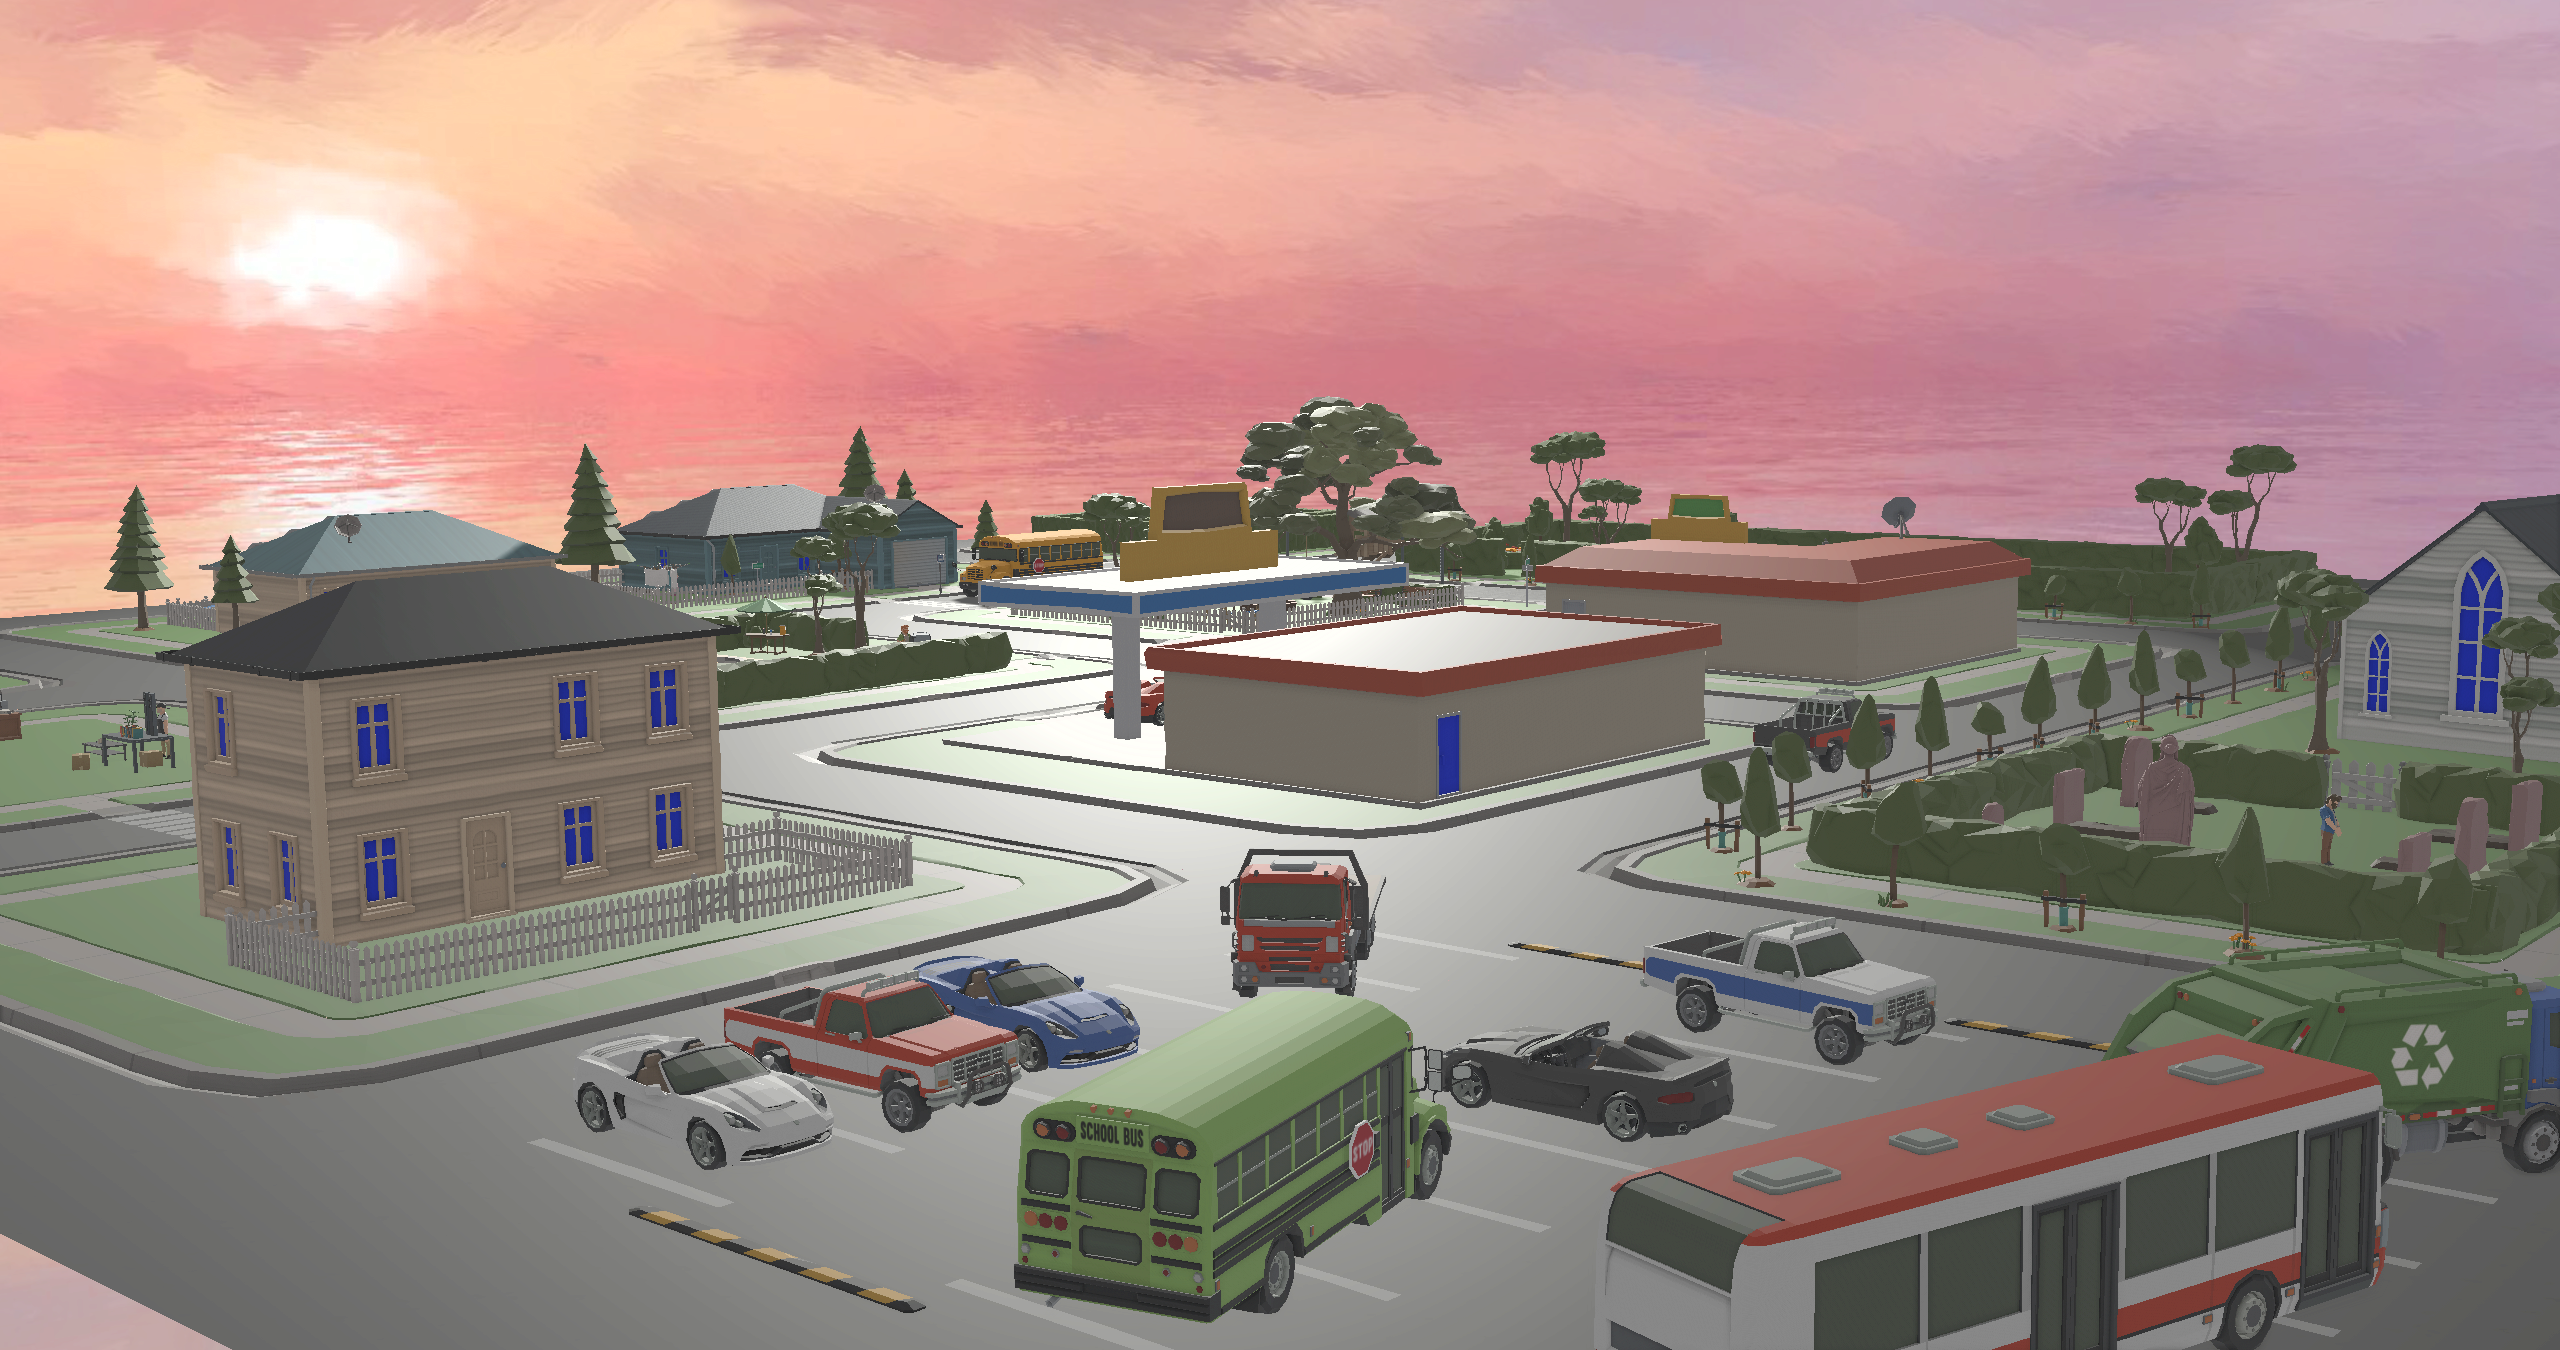
\includegraphics[width=0.5\textwidth]{images/map1.png}
  \caption{This is an example ToDo picture.}
  \label{fig:todo}
\end{figure}


\begin{figure}[]
  \centering
  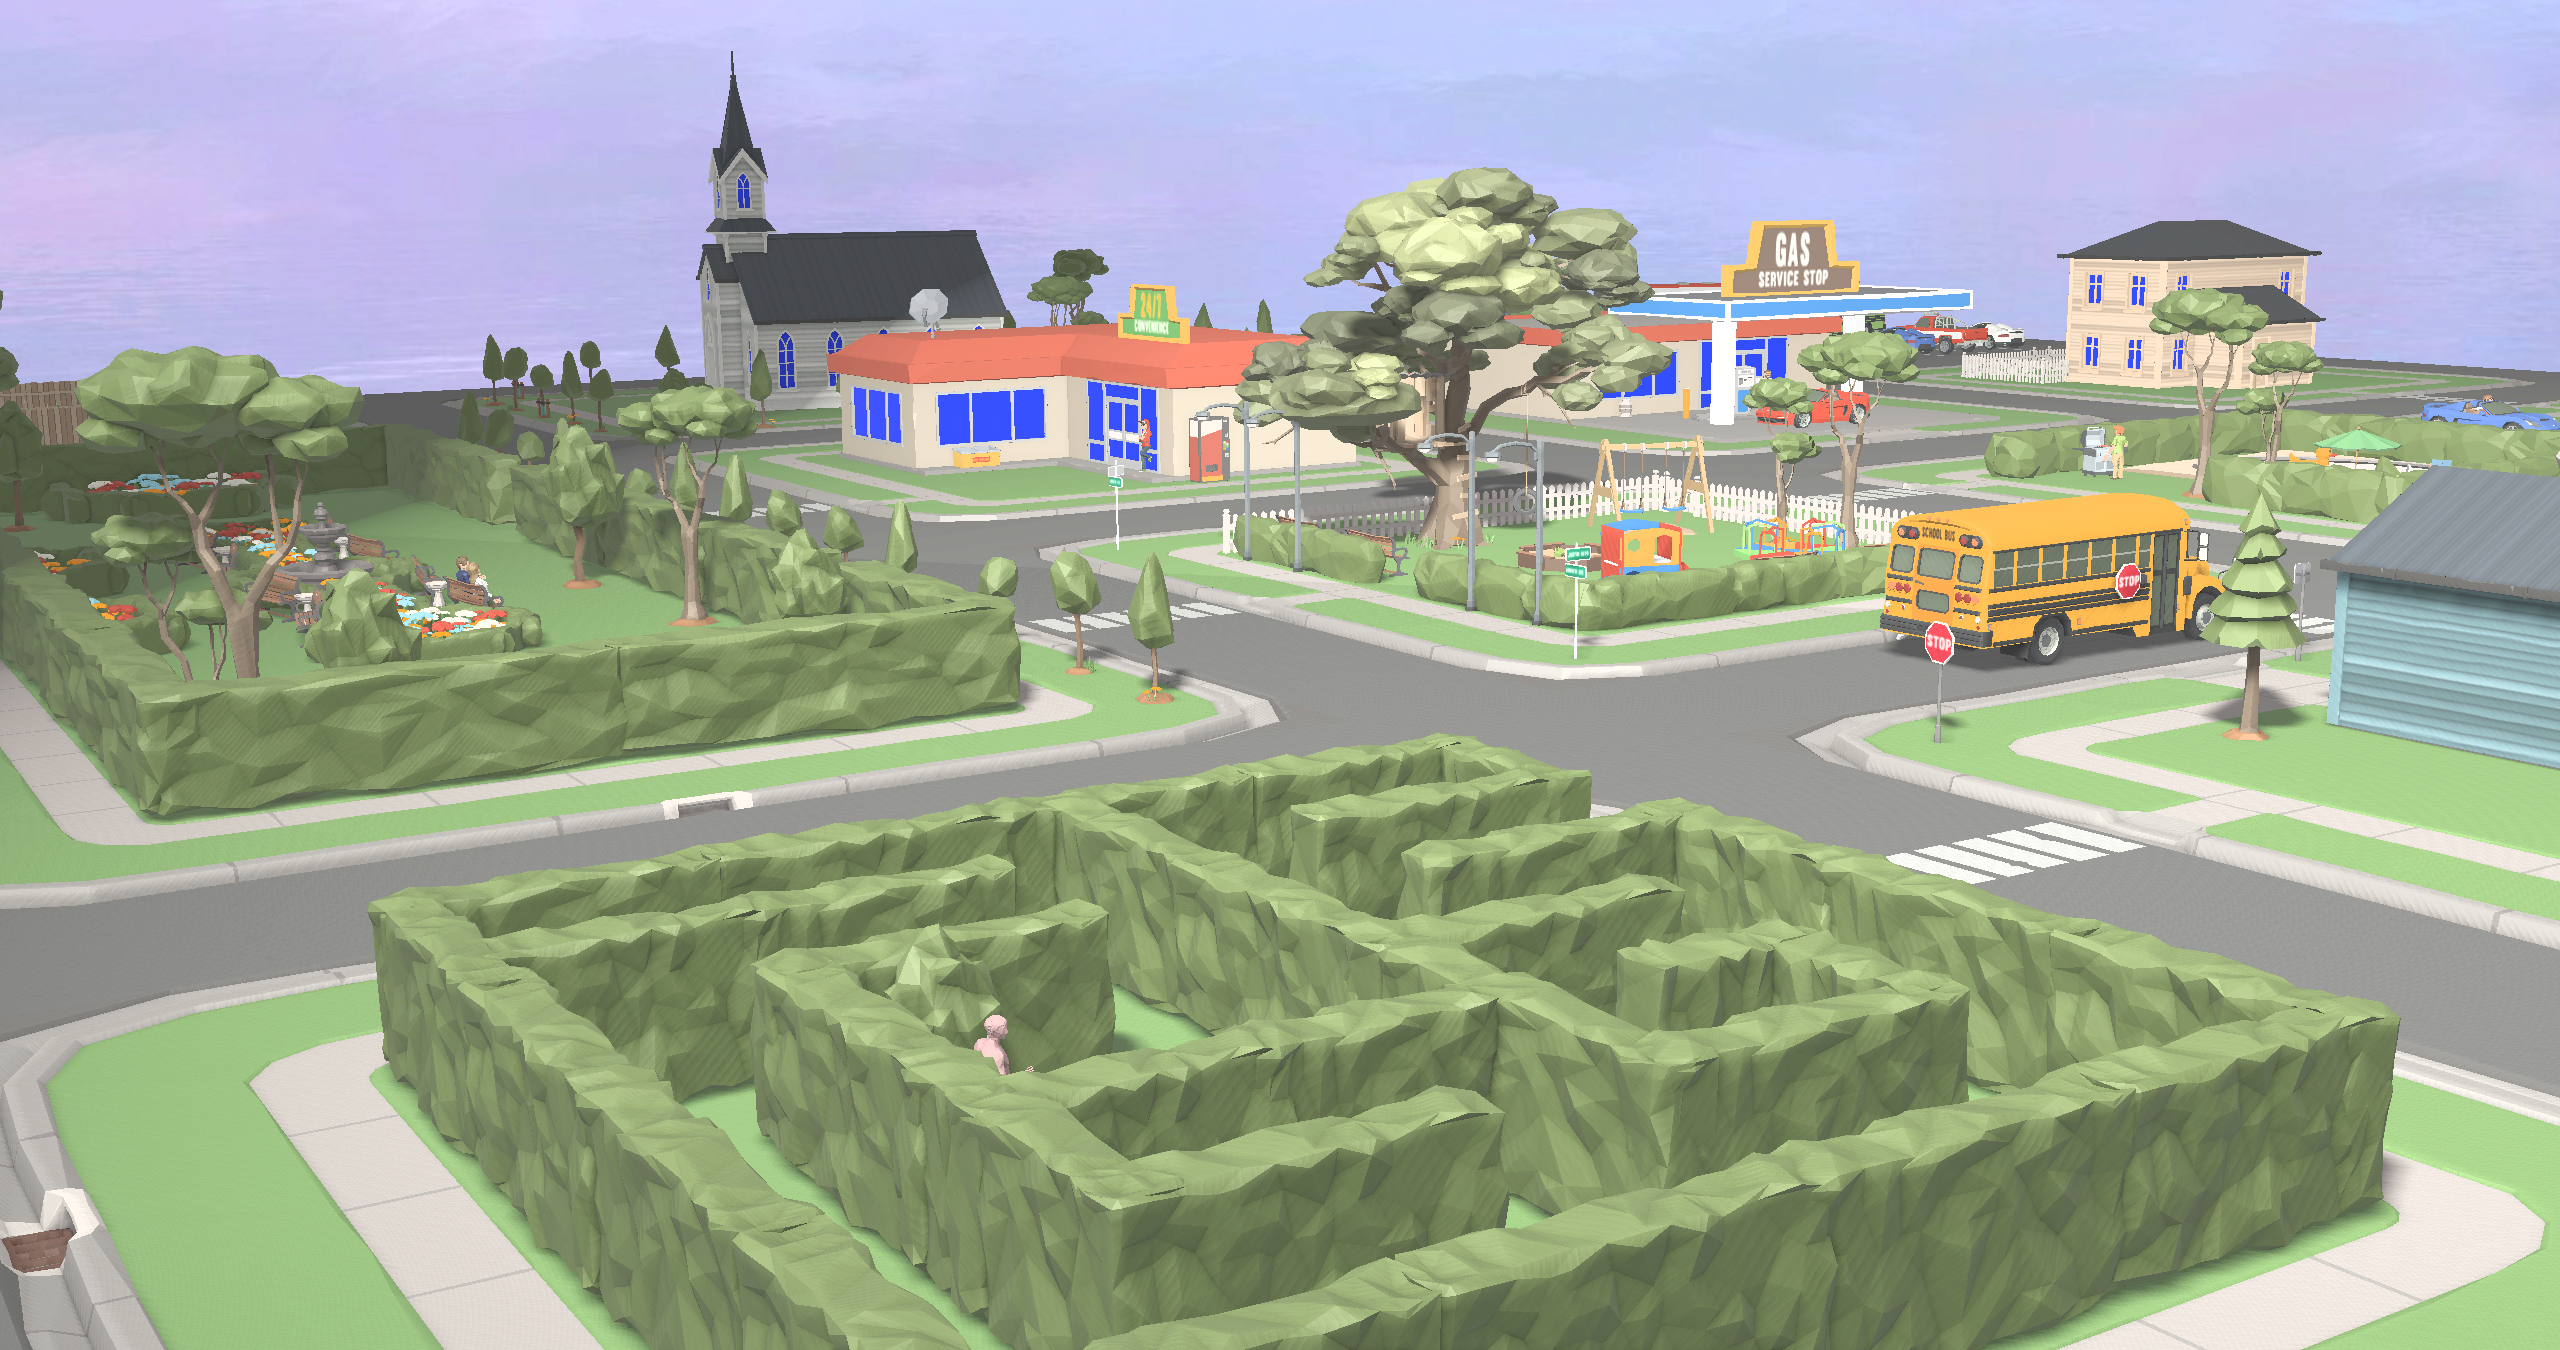
\includegraphics[width=0.5\textwidth]{images/map2.png}
  \caption{This is an example ToDo picture.}
  \label{fig:todo}
\end{figure}

Um eine geeignete Testumgebung zu erhalten wurde im Rahmen einer HiWi-Stelle eine Nachbarschaft gebaut, welche sich dadurch auszeichnet, dass sie aus einzelnen "Inseln" besteht, welche einfach umgestellt werden können. Das genutzte Asset-Pack\footnote{https://www.cgtrader.com/3d-models/exterior/house/polygon-town-pack} kommt mit der Nutzung von sehr wenigen Polygonen aus, was die Rechenleistung bei der Bildberechnung auf der Grafikkarte minimiert und somit für schnellere Hertzraten sorgt.

\chapter{Interaktionsdesign}
Nachdem die grundlegende Herangehensweise der Technik geklärt wurde, wird in diesem Kapitel auf Design- und Konzeptionsideen eingegangen, die bis zur finalen Umsetzung aufkamen. Die meisten der verschiedenen Umsetzungsmöglichkeiten wurden bei der Entwicklung getestet und ihre Praktikabilität analysiert, woraus sich das im letzten Unterpunkt beschriebene, finale Interaktionsdesign für eine mögliche Studie abgeleitet wurde.

\section{Module}
Die Technik besteht aus den folgenden vier Grundbausteinen: Der World in Miniature, der miniaturisierten Nutzerplattform in der WIM, einem Selektionstool und dem Portalfenster.

\textbf{WIM:}\\
Die verwendete WIM soll in unserem Fall eine exakte Kopie der Umgebung sein und nicht wie bei Pierce et al. aus einer vereinfachten Version bestehen. Die Nutzer sollen in der Lage sein, auch feinere Details in der WIM erkennen zu können. 

 \textbf{Selektionstool:}\\
Um die Technik nutzen zu können bedarf es eines Werkzeugs, mit welchem der Nutzer mit der WIM interagieren kann. 

\textbf{Minaturisierte Nutzerplattform:}\\
\begin{figure}[h!]
  \centering
  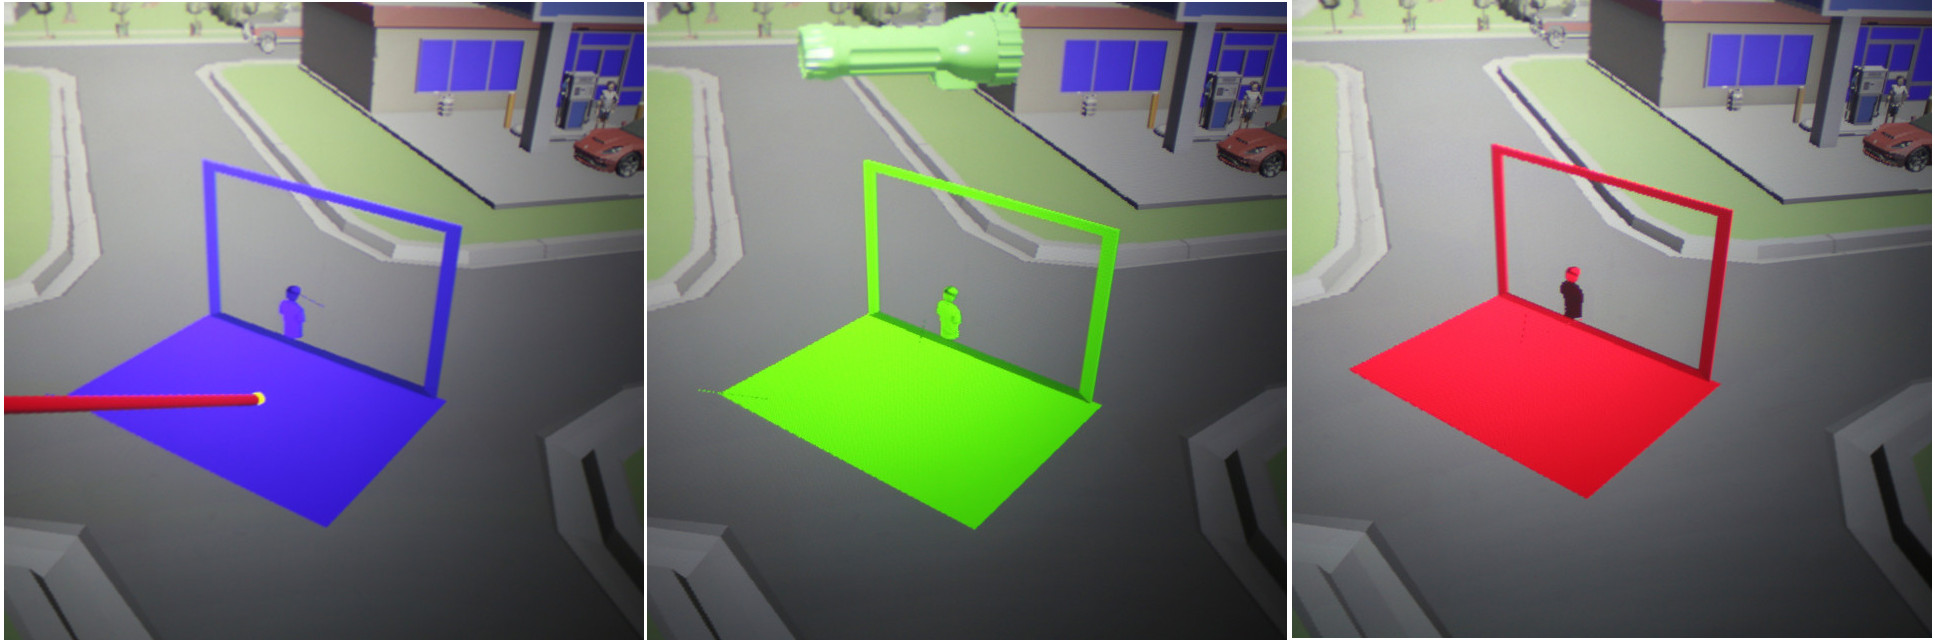
\includegraphics[width=0.8\textwidth]{images/platform_bgr.jpg}
  \caption{Die drei Versionen der Nutzerplattform in der WIM: Die Blaue dient zur Planung der Position in der WIM. Wird diese bestätigt wird eine grüne Kopie erstellt. Nach dem Teleport zeigt die rote Plattform den tatsächlichen, aktuellen Aufenthaltsort der Nutzer in der Umgebung an}
  \label{fig:todo}
\end{figure}
Die miniaturisierte Nutzerplattform (im Folgenden: Plattform) repräsentiert die Nutzer (in Form von Avataren), die 3D-Leinwand sowie die Bodenplatte, welche den getrackten Bereich des realen Raumes darstellt. Diese Plattform ist in der WIM zum Beispiel an der Stelle (in rot, vgl. Abbildung 8.1) sichtbar, an denen sich die Nutzer zu diesem Zeitpunkt befinden, damit sie ihre aktuelle Position in der Umgebung einschätzen können. Dabei ist es wichtig, dass die Tracking-Koordinaten, welche die Positionen der Köpfe der Nutzer bestimmen in dieser Version aktualisiert werden, damit die Avatarpositionen denen der Nutzer im realen Raum entsprechen. Eine zweite Form dieser Repräsentation soll nämlich auch zur Reiseplanung dienen. Indem diese Plattform vom steuernden Nutzer in der WIM platziert wird, spezifiziert er die Position, an der sich die Nutzergruppe nach dem Teleport befinden soll.

\textbf{Portalfenster:}\\
Das Portalfenster (oder \textit{Peephole}) zeigt nach der Platzierung der Preview-Plattform einen Ausschnitt des Ortes, an den gereist werden soll. Dabei erhält jeder seine eigene Perspektive durch dieses "Loch". Das ermöglicht jedem Nutzer durch Veränderung seiner Position eine andere Perspektive in die Welt "hinter" dem Loch (vgl. Abbildung 8.8)

\section{Position der WIM}
Eine zentrale Frage, die es zu beantworten galt, war, wo genau die WIM in der Szene sichtbar ist. Drei Herangehensweisen waren dabei naheliegend:

\subsection{In der Hand}

\begin{figure}[h!]
  \centering
  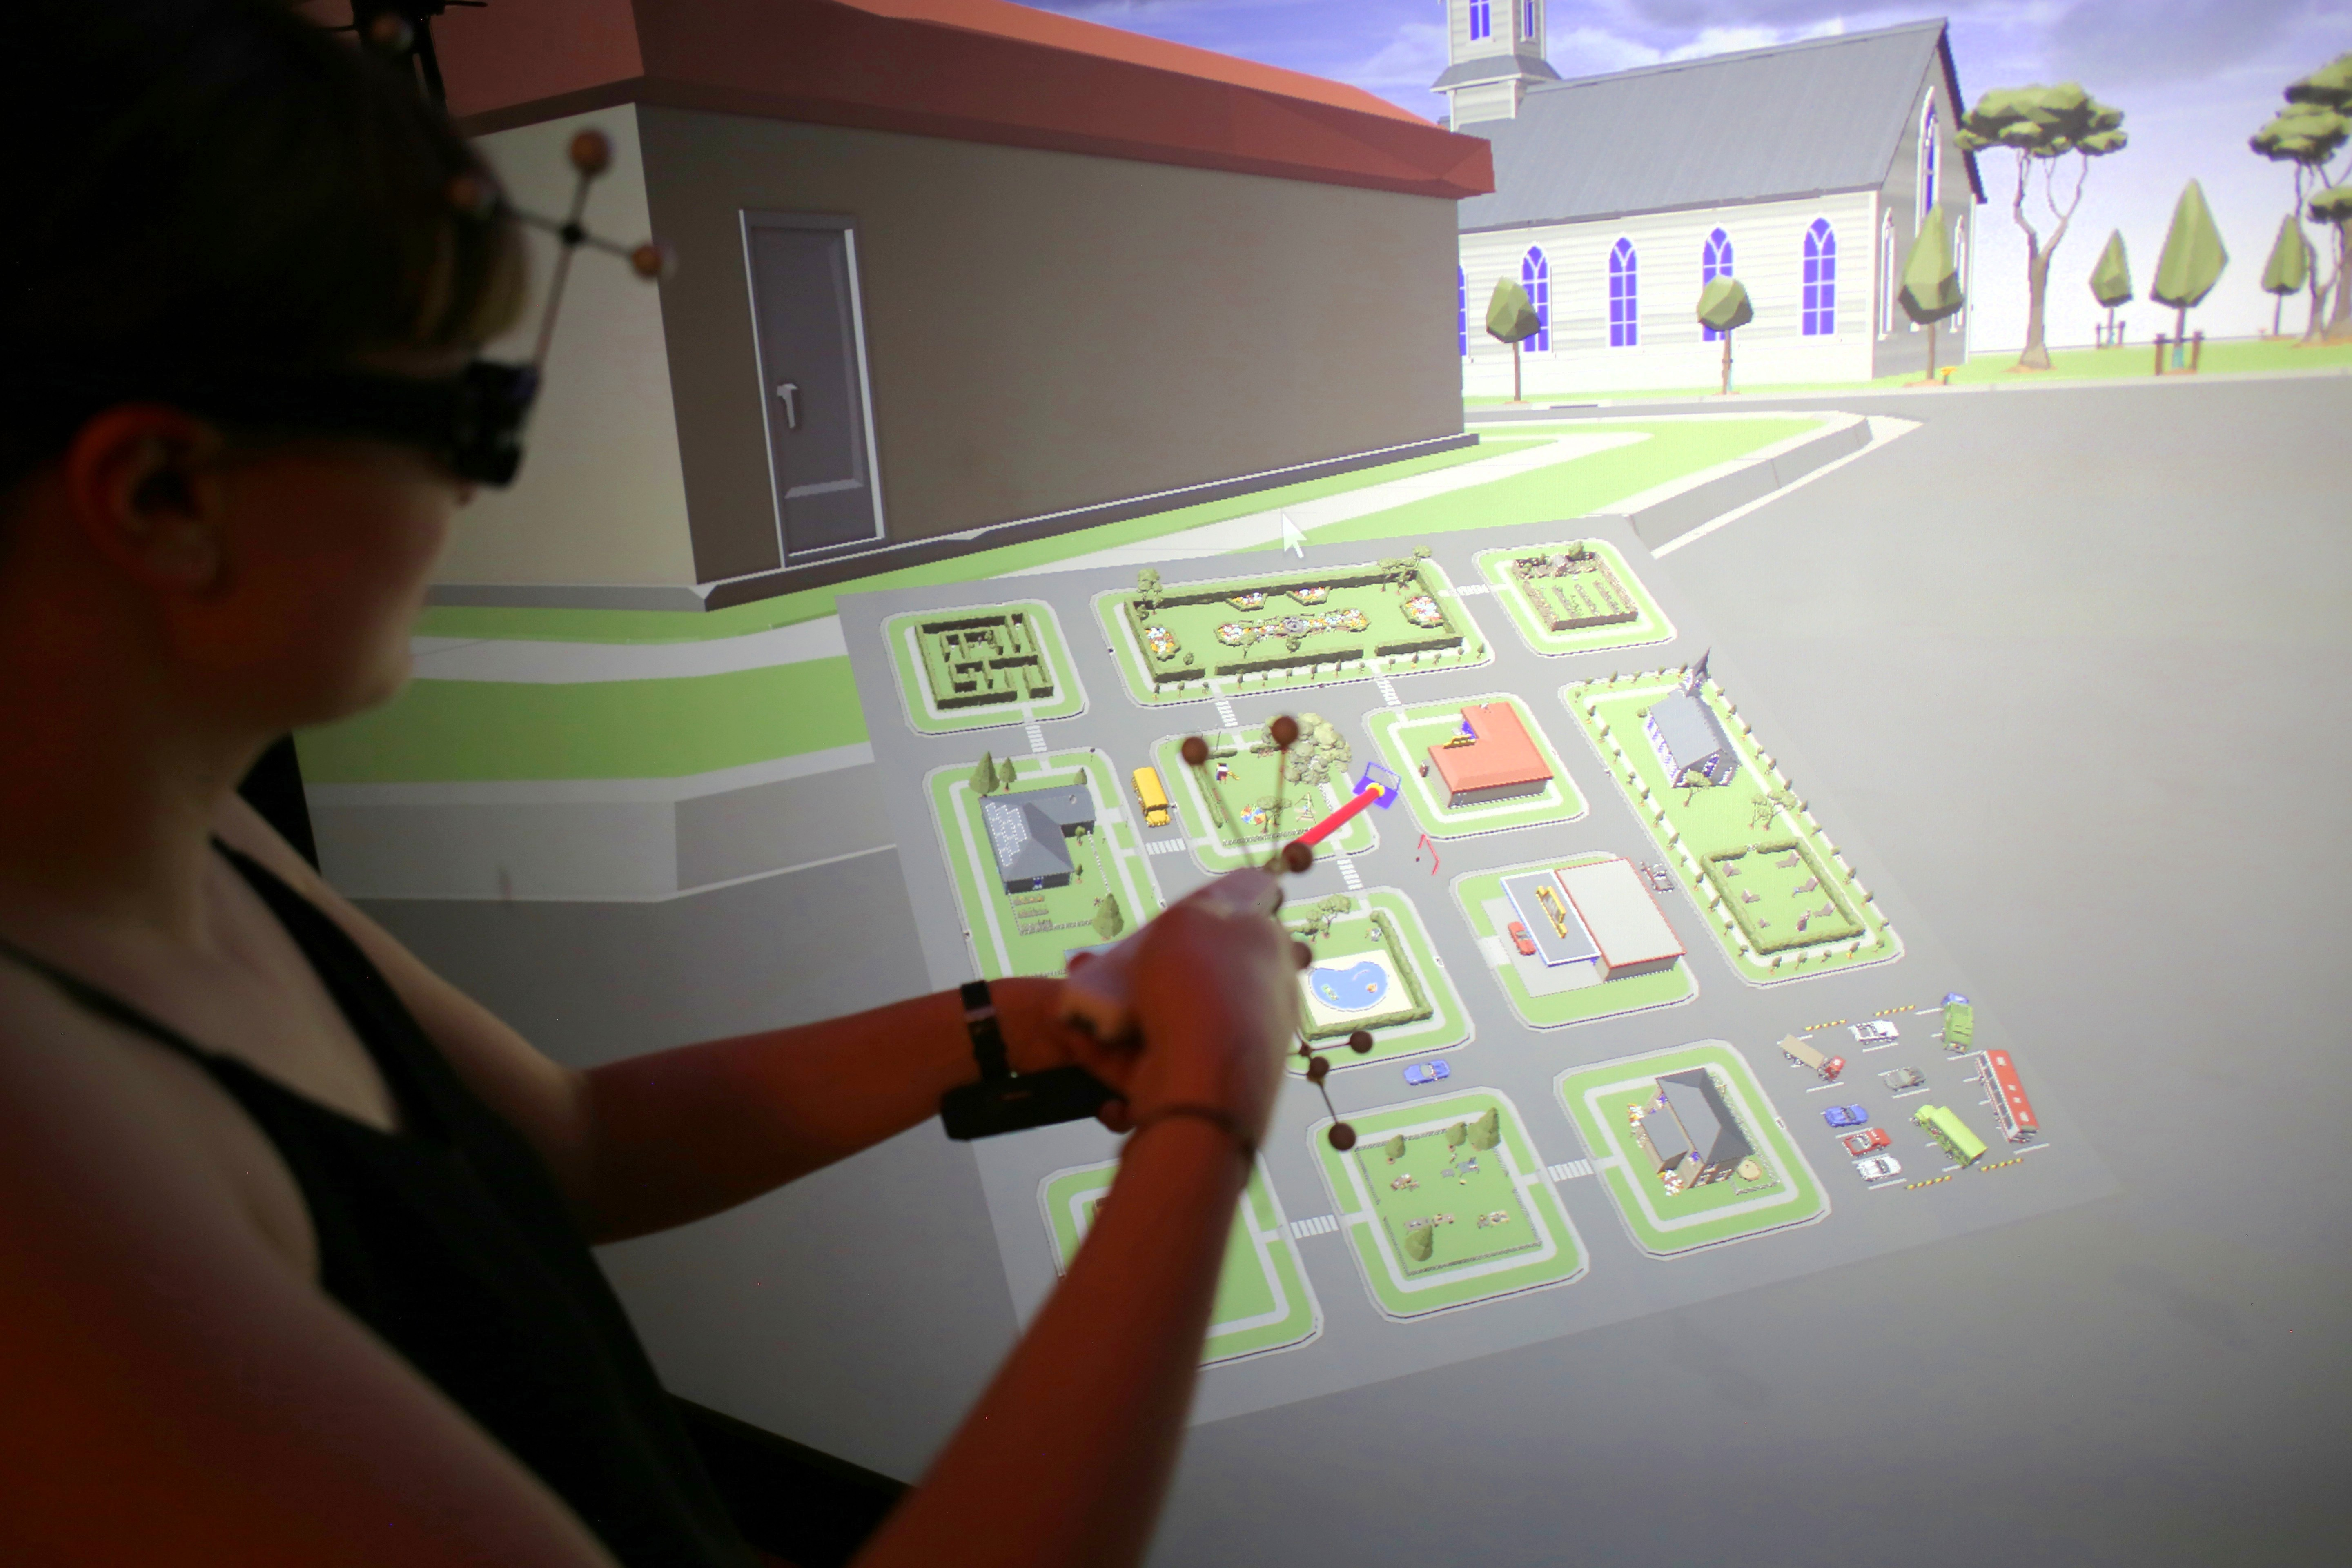
\includegraphics[width=0.8\textwidth]{images/wim_in_hand.JPG}
  \caption{Hält ein Nutzer die WIM in der Hand, so kann er sie sehr intuitiv bedienen. Allerdings könnte er sie für andere verdecken.}
  \label{fig:todo}
\end{figure}

Die erste Herangehensweise war, die WIM an einen getrackten Gegenstand zu koppeln. In diesem Fall bestand dieser aus einem Holzwürfel mit fünf reflektierenden Kügelchen.
Dies ermöglicht verschiedene Szenarien einfach durch zu spielen, indem man den Holzwürfel an verschiedenen Stellen im Raum platziert oder ein Nutzer diesen in die Hand nimmt.

Mit der WIM in der nicht-dominanten Hand kann der Nutzer diese sehr gut drehen und sie somit aus (fast) allen Richtungen einsehen. Dabei kann er mit seiner dominanten Hand die gewünschte Position auswählen. Dieses Zusammenspiel mit der groben Justierung der WIM in der linken und der feingliedrigen Interaktion mit der rechten Hand funktioniert sehr natürlich.
In unserer Testversion wurde die WIM stets unsichtbar gestellt, sobald der Holzwürfel unterhalb der Hüfte gehalten wurde.

Der steuernde Nutzer hält die WIM nämlich oft so, dass die wichtigen Punkte für ihn sichtbar sind, jedoch nicht zwangsläufig für die anderen Nutzer. Dies kann noch verschlimmert werden, wenn die WIM durch den Körper der Person verdeckt wird.


\subsection{Tabletop}
Eine weitere Möglichkeit ist die Platzierung der WIM auf einem Holotisch, wie er in unserem Labor verfügbar ist.
Dadurch wäre die WIM für alle sichtbar und gleichzeitig nicht im Sichtfeld auf die Hauptszene. Gleichzeitig bedeutet dies allerdings, dass bei jedem Navigationsvorgang die Aufmerksamkeit der Nutzer von der Szene zum Tisch wandern muss, was denn Interaktionsfluss stören kann. Diese Option wurde im Rahmen der Arbeit nicht implementiert.

\subsection{Zentral, Mitte der Nutzergruppe}


\begin{figure}[h!]
  \centering
  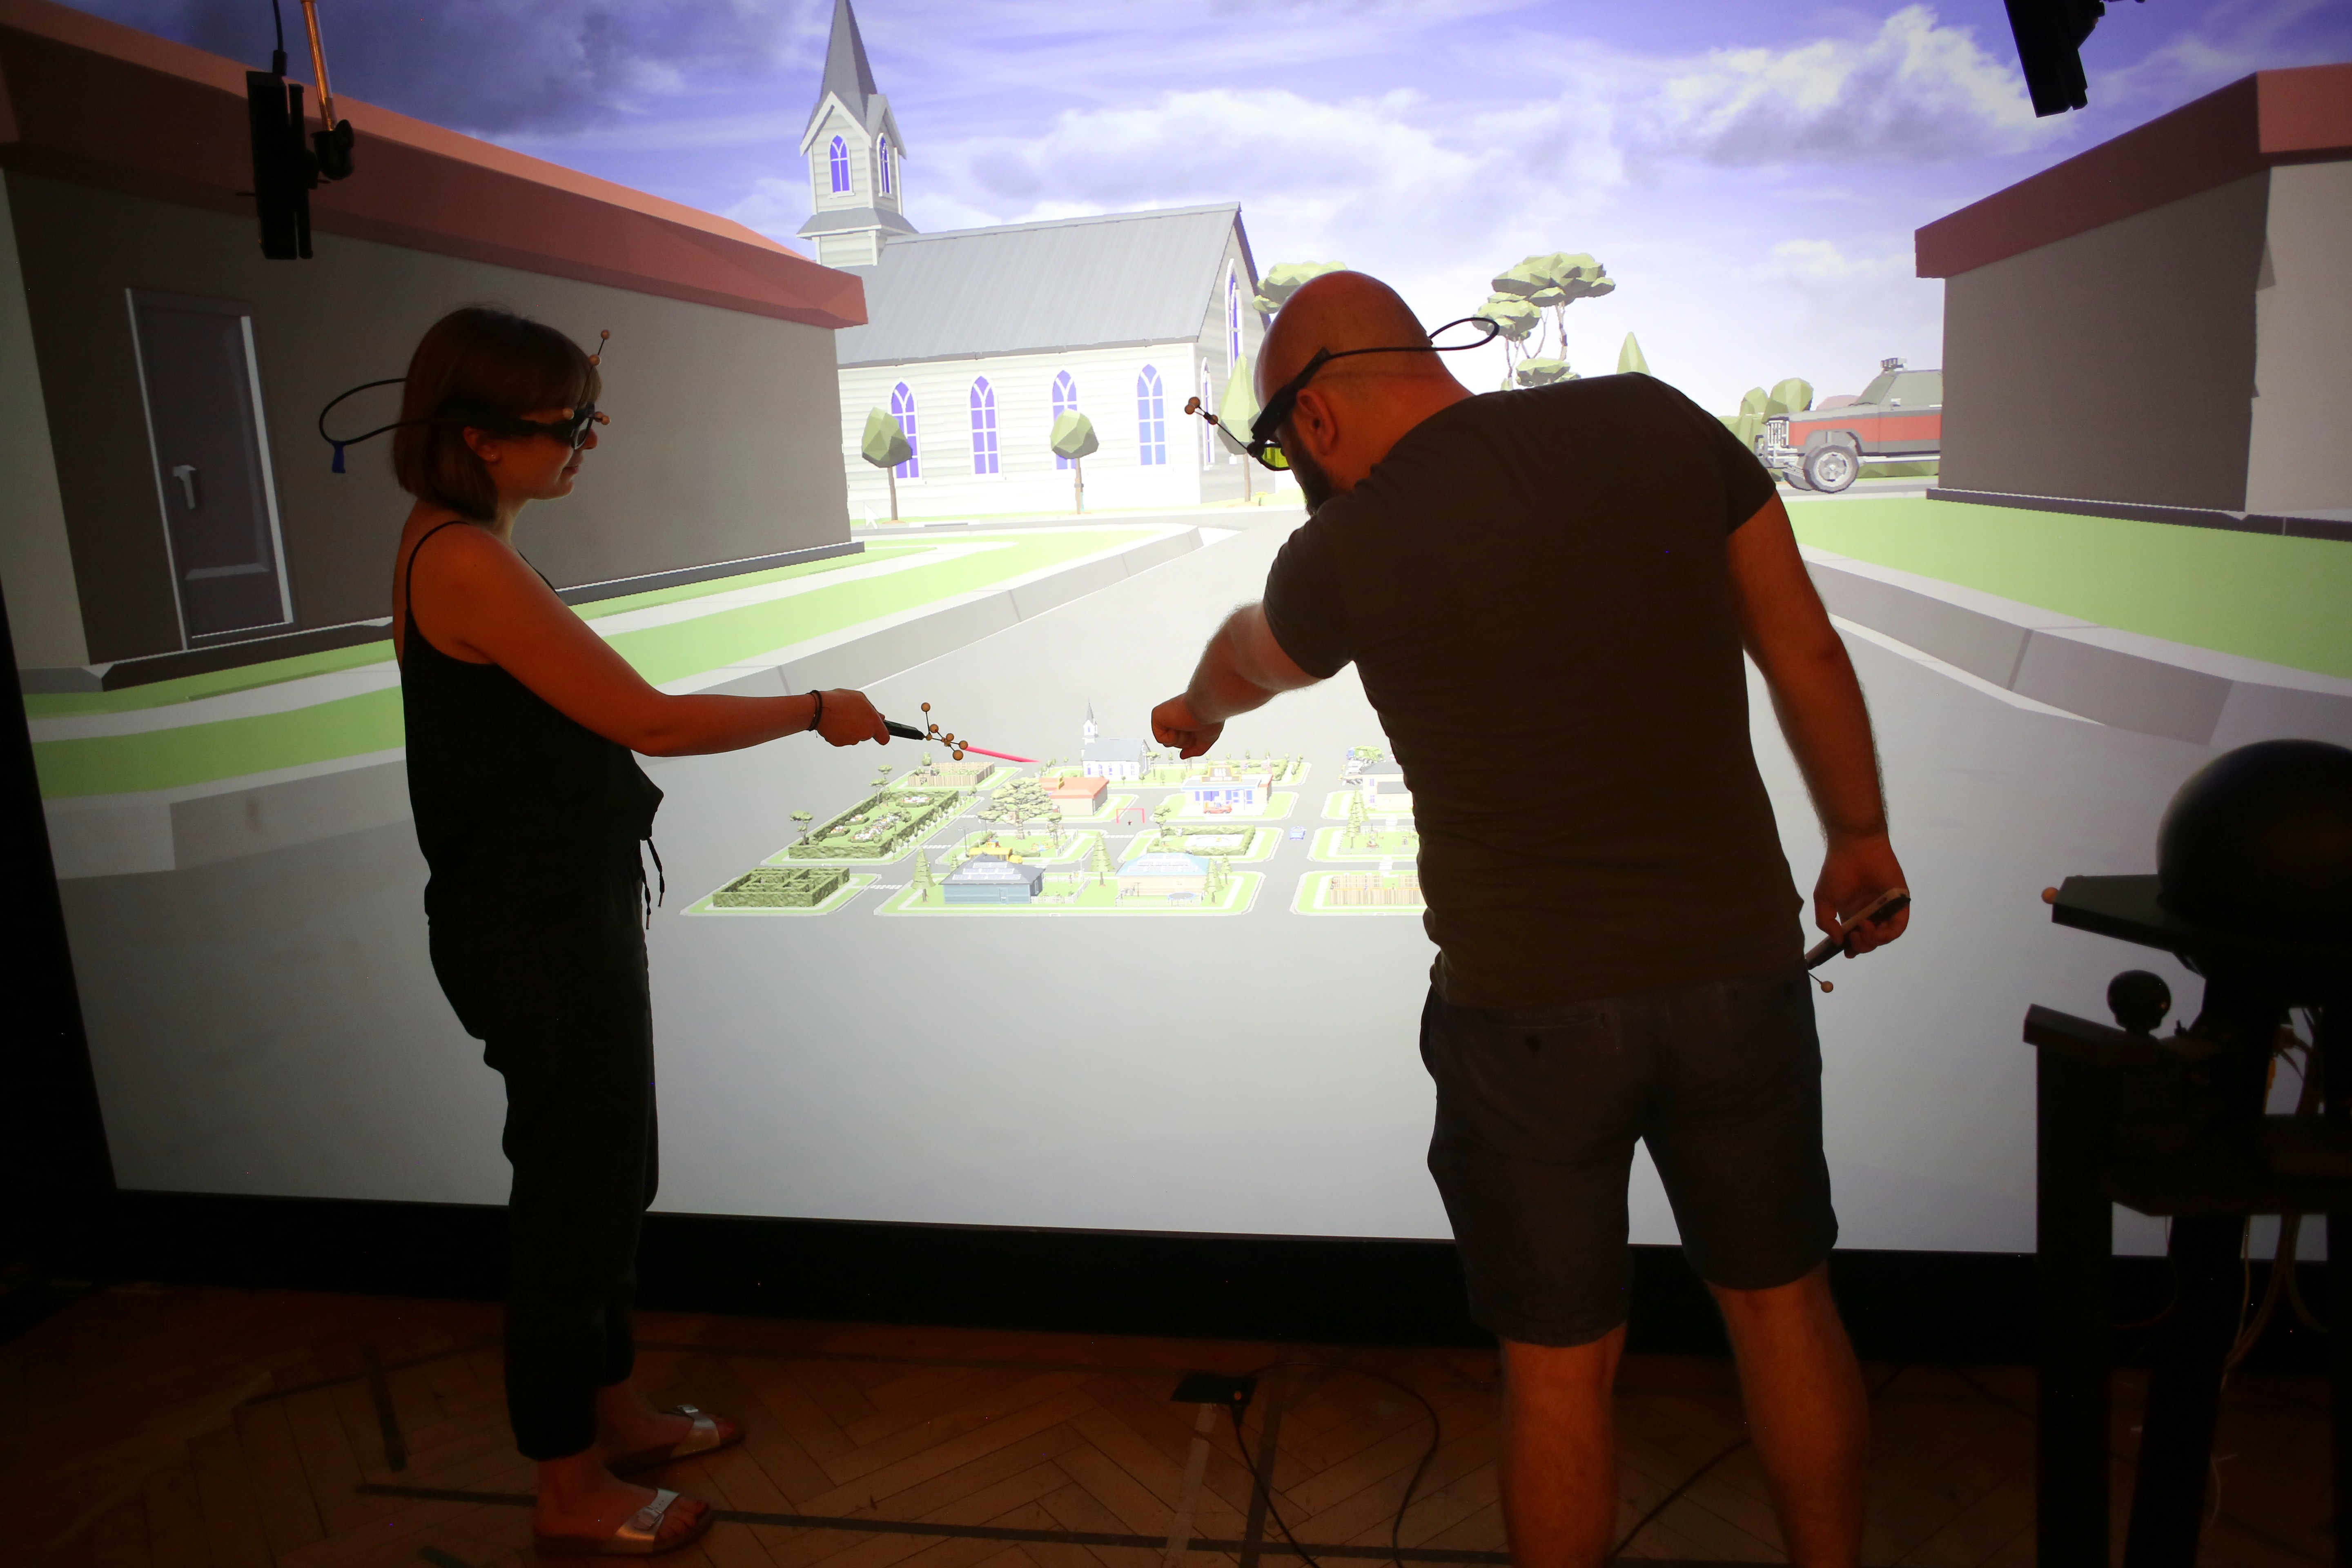
\includegraphics[width=0.8\textwidth]{images/wim_zentral.JPG}
  \caption{Steht die WIM zentral zwischen der Nutzergruppe, ist sie für alle einseh- und bedienbar.}
  \label{fig:todo}
\end{figure}

Stellt man die WIM zentral vor die Nutzergruppe (also kurz vor die Leinwand) bringt dies den Vorteil mit sich, dass sie von allen Nutzern gut eingesehen werden kann.
Dabei ist es von Nöten, dass sie durch eine zusätzliche Eingabe drehbar ist, da man sonst Teile, die nur von der Rückseite der Leinwand aus sichtbar wären, nicht auswählen kann.
In unserem Fall wurde dies durch das Drehen eines Joysticks am Spheron ermöglicht.
Als optimale Höhe stellte sich dabei ungefähr 1,30 Meter heraus. So kann man die WIM gut überblicken und muss sich gleichzeitig nicht zu weit bücken

Angelehnt an Kunert et al. \cite{Kunert2014Photoportals} wurde ebenfalls eine Möglichkeit implementiert, bei der sich die WIM sowohl in der Hand, als auch in zentraler Position befindet. Solange ein Nutzer den Holzwürfel in der Hand hat, befindet sich die WIM ebenfalls dort. Stellt er ihn in der Nähe des Spherons ab, wird die WIM mit diesem gekoppelt und befindet sich ab diesem Moment in der oben beschriebenen Zentralposition.

\subsection{Projektion am Boden}
Wie bereits im vierten Kapitel beschrieben, wäre es ebenfalls denkbar, die WIM mit einer Projektion am Boden darzustellen, wie bei Stoakley et al. \cite{Stoakley2010VirtualWIM}.
Damit hätte man den Vorteil, dass die WIM direkt bedient werden könnte und gleichzeitig nicht im Weg ist. Grundsätzlich kann die WIM dabei zwei- und dreidimensional sein (wobei letzteres für Mehrbenutzer einen extremen Mehraufwand auf Hardwareseite mit sich bringen würde). Diese Variante wurde im Zuge dieser Arbeit wegen des hohen technischen Aufwandes nicht implementiert.

\section{Größe der WIM}
Die quadratische Testumgebung hat eine Seitenlänge von 125 Metern, wobei nur der zu bereisende Bereich eine Größe von etwa 100 Metern aufweist.
Der Maßstab wird dabei 1:100 gewählt. Mit dieser Größe können alle Teile der WIM gut erreicht werden und die miniaturisierte Plattform ist mit einer Breite von 5 cm gut erkennbar. 
Dennoch wird den Nutzern die Möglichkeit gegeben, die Skalierung der WIM zu ändern. Dies wird erreicht, indem der Nutzer mit gedrückten Skalierungsknopf seinen Pointer vom Zentrum der WIM weg oder auf dieses zu bewegt. Dabei wird die Skalierung entsprechend des Verhältnisses von der aktuellen Distanz zum Zentrum und der Ausgangsdistanz gewählt (Beispiel: Der Nutzer drückt in einer Distanz von einem Meter von Zentrum den Knopf und verringert die Distanz auf 50 Zentimeter. Die WIM wird folglich um die Hälfte herunterskaliert).

Die Größe der WIM hat eine wichtige Auswirkung auf die Bedienbarkeit der Technik und somit auch der Bearbeitungszeit der Technik. Im folgenden Kapitel (9.1.1) wird darauf näher eingegangen.

\section{Platzierung der Nutzerplattform}
Um das Ziel der Reise zu bestimmen soll die Plattform so platziert werden können, dass jede mögliche und gewünschte Position und Orientierung erreichbar ist., wobei der Aufwand der Platzierung minimal gehalten werden soll.

\subsection{Positionierung in der Luft}

\begin{figure}[h!]
  \centering
  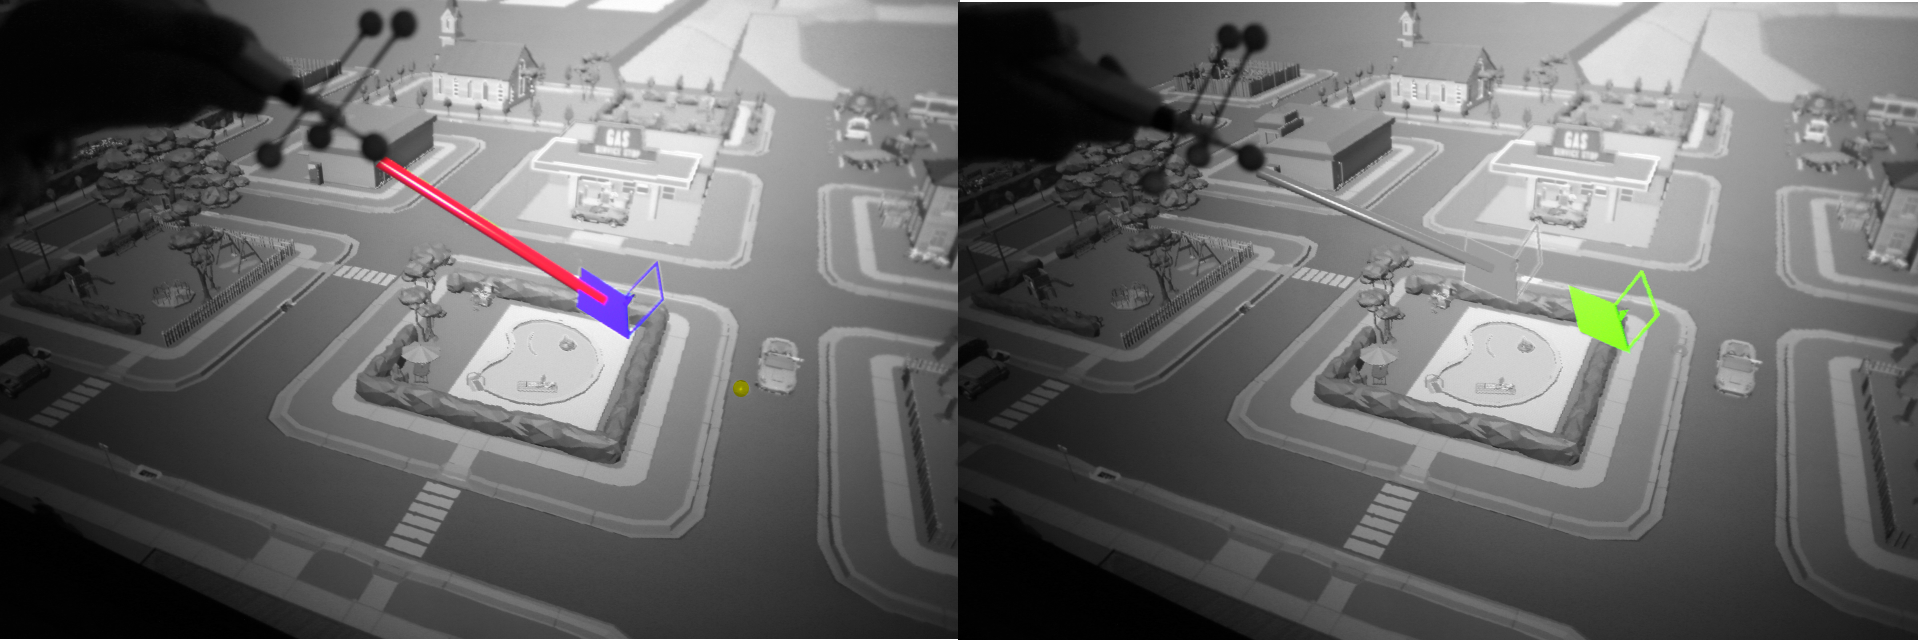
\includegraphics[width=0.8\textwidth]{images/fork.png}
  \caption{Mit der Gabeltechnik ist es möglich die Plattform in der Luft zu positionieren. Dabei visualisiert der gelbe Punkt die Blickrichtung. Auf Knopfdruck wird diese Position bestätigt und die grüne Plattform zeigt die Position nach dem Teleport.}
  \label{fig:todo}
\end{figure}


Um die Plattform in der WIM zu platzieren, sodass sie schwebend mit freier Rotation im Raum steht, wurde eine Art \textit{Gabel-Technik} entwickelt. Hierbei wird an das Ende des Pointers ein kurzer (ca. 20cm) Strahl gehängt, an dessen Ende sich die Miniatur befindet (in der Abbildung in blau zu sehen). Wird die aktuelle Position dieser Repräsentation in der WIM durch einen Klick bestätigt, wird eine Kopie erstellt, die die finale Position widerspiegelt, die die Nutzer nach der Reise haben werden (siehe in Grün in der Abbildung).
Somit ist es den Nutzern möglich ihre Orientierung und Position in der Welt frei zu bestimmen, um z.B. auch von oben auf Gebäude blicken zu können.


\subsection{Positionierung am Boden}
Will die Nutzergruppe entlang des Bodens ausgerichtet bleiben, bieten wir folgende Möglichkeiten:

\subsubsection{Direkte Auswahl}

\begin{figure}[h]
  \centering
  \includegraphics[width=0.8\textwidth]{images/direct.png}
  \caption{Direkte Auswahl: Für die schnelle und effiziente Auswahl wird die Plattform, sobald man den Boden schneidet, entlang der Strahlrichtung ausgerichtet.}
  \label{fig:todo}
\end{figure}

Berührt die blaue Plattform der \textit{Gabel-Technik} den Boden, so wird sie automatisch entlang diesem ausgerichtet. Die Sichtrichtung der Gruppe ist dabei immer entlang der, in die Bodenebene projizierten, Strahlrichtung vom Pointer weg. Dadurch wird eine sehr direkte Form der Positions- und Richtungsauswahl ermöglicht, die man mit einem kurzen Knopfdruck bestätigen kann. Auch in diesem Fall wird eine grüne Kopie der vormals blauen Plattform erstellt.

\subsubsection{Position und Blickrichtung}

\begin{figure}[h]
  \centering
  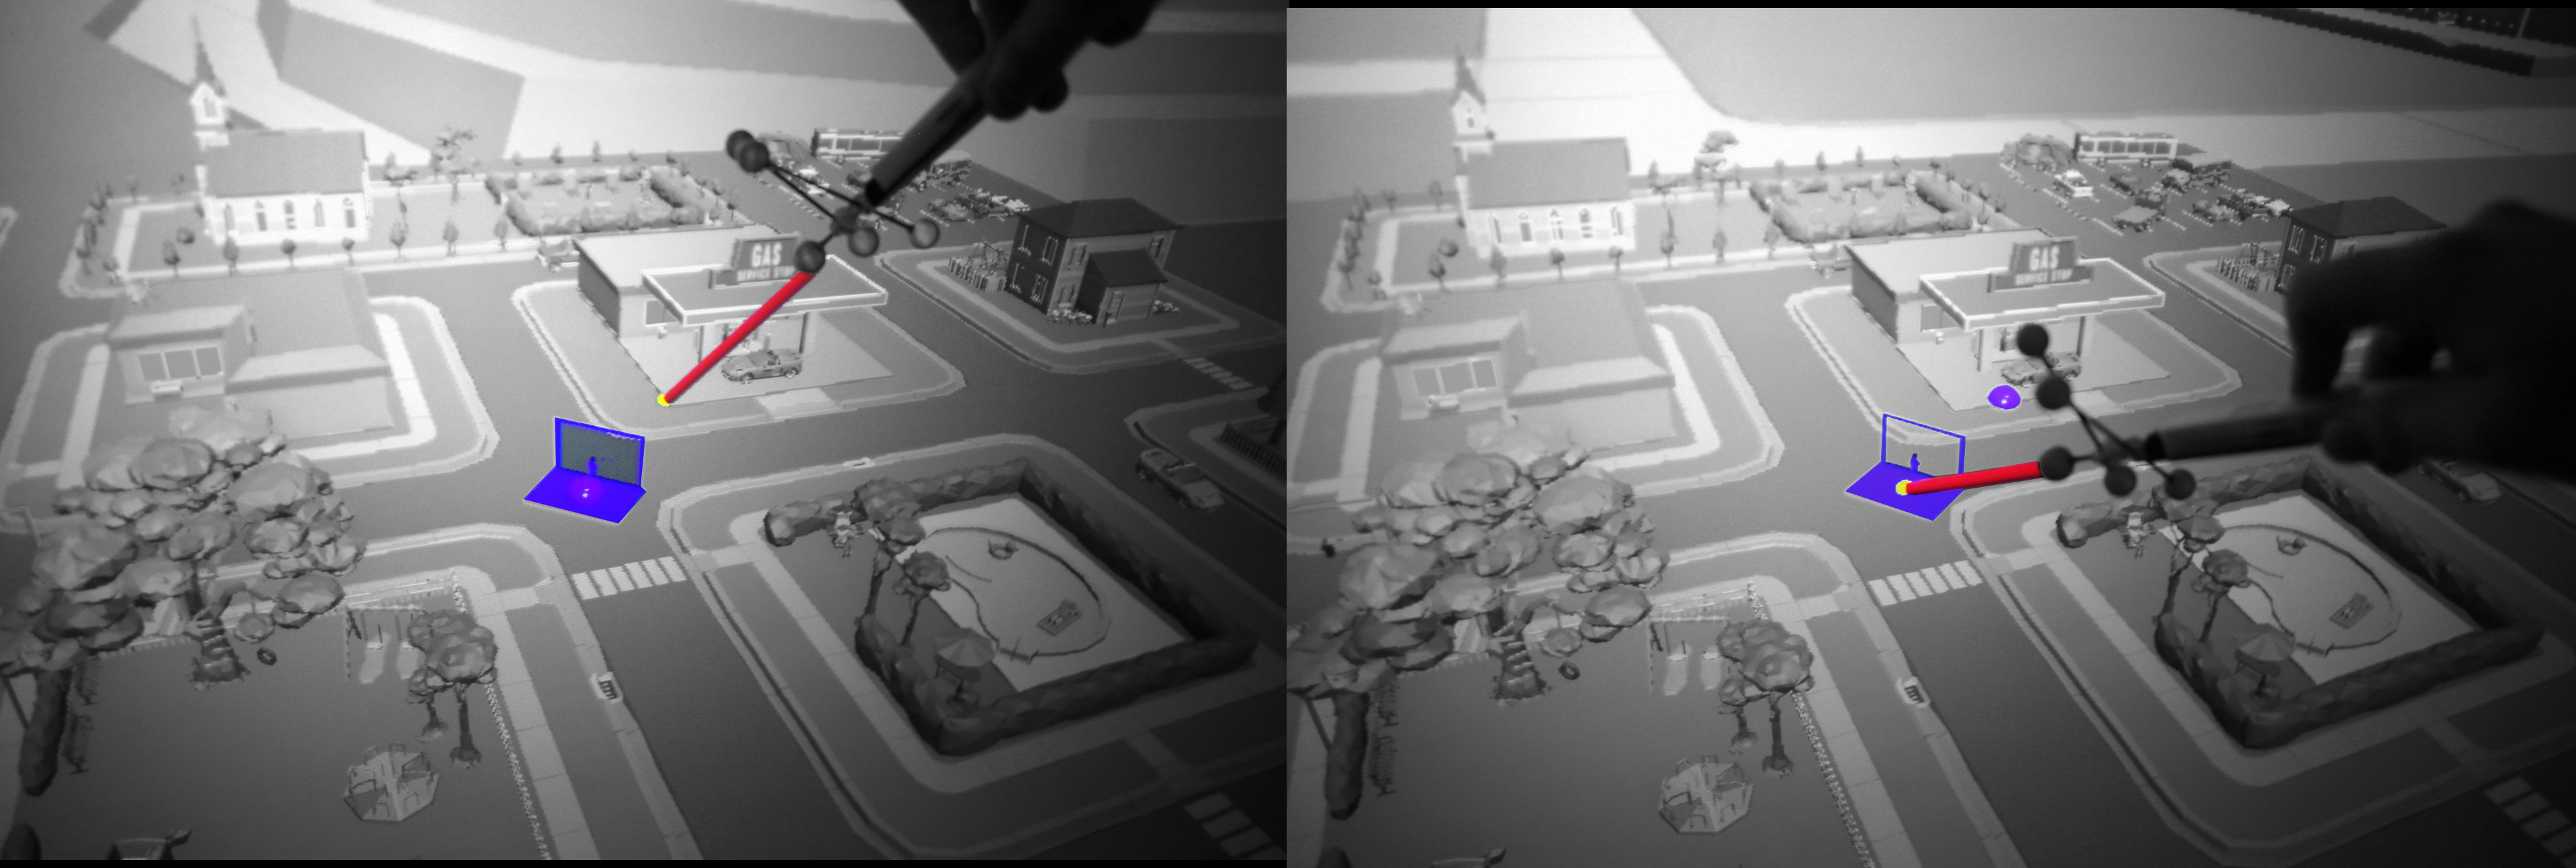
\includegraphics[width=0.8\textwidth]{images/look.jpg}
  \caption{Position und Blickrichtung: Hält man den Knopf länger gedrückt, während man den Boden schneidet bietet das System zwei Möglichkeiten: Entweder die Plattform wird an den aktuellen Punkt gesetzt und man bestimmt fortan die Blickrichtung (links) oder man wählt erst den Punkt den man sehen will und positioniert danach die Plattform, die dann immer in Richtung dieses Punktes ausgerichtet ist (rechts)}
  \label{fig:todo}
\end{figure}


Hält man den Knopf allerdings länger gedrückt, so bestätigt man, dass der aktuelle Schnittpunkt mit der WIM der Punkt ist, den man gerne sehen möchte. Hält man den Knopf nun weiterhin gedrückt, kann man die Position der Plattform wählen, wobei diese immer in Richtung des Anfangs gewählten POI ausgerichtet ist.
Natürlich ist es auch möglich, eine umgekehrte Version dieser Technik zur Verfügung zu stellen. In diesem Fall wird durch langes Drücken erst die Position der Plattform gewählt, welche dann in Richtung des aktuellen Schnittpunkts mit der WIM ausgerichtet wird. 
Generell lässt sich aber sagen, dass die erste Methode in den meisten Fällen als etwas besser bedienbar eingeschätzt wurde, da man damit sicherstellen kann, dass wirklich alle Bestandteile des POI`s innerhalb des sichtbaren Bereichs sind.

\subsection{Plane of Interest}

Zusätzlich zu den Platzierungstechniken, die bisher beschrieben wurden, gibt es weiterhin die Möglichkeit, sogenannte \textit{Planes of Interest} zu erstellen. Diese sind ebenfalls Kopien der Nutzerplattformen, welche frei in der WIM positioniert werden können. Die Platzierung funktioniert dabei kontextabhängig:
Zeigt der Nutzer in die WIM, so läuft sie analog zu den in den vorherigen Unterpunkten beschriebenen Vorgängen ab, wobei durch den Klick eines anderen Knopfes (\textit{PLOI-Knopf}) keine grüne, sondern eine weiße Plattform erscheint. Schneidet man zukünftig diese mit dem Selektionsstrahl, so erhält die blaue Plattform die Ausrichtung und Position der weißen.

\begin{figure}[h!]
  \centering
  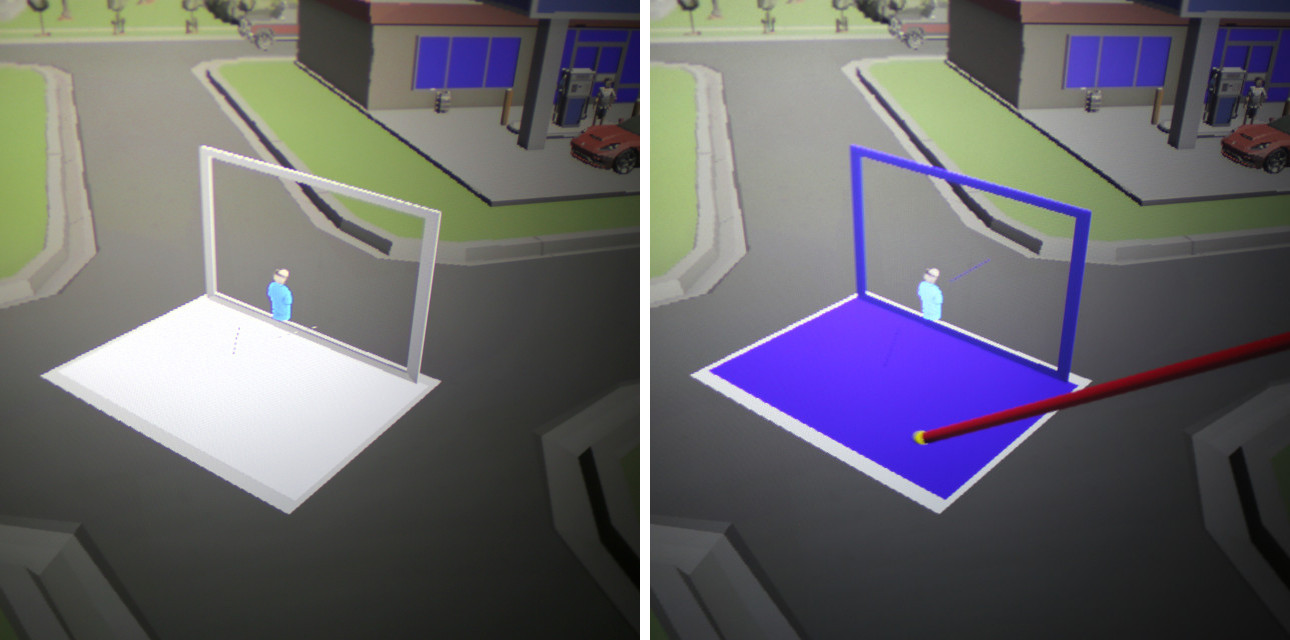
\includegraphics[width=0.8\textwidth]{images/platform_bluewhite.JPG}
  \caption{Mit der sogenannten \glqq Plane of Interest\grqq{}, lassen sich Aufenthaltsorte speichern. Schneidet man diese weißen Plattformen mit dem Selektionsstrahl so wird die blaue Plattform direkt entsprechend der weißen ausgerichtet.}
  \label{fig:todo}
\end{figure}

Dadurch lassen sich für später oder für andere Nutzer Orte speichern, die dann ohne großen Aufwand angesteuert werden können.
Zeigt der Nutzer allerdings nicht in die WIM, so wird auf Knopfdruck der aktuelle Aufenthaltsort gespeichert, indem ebenfalls eine weiße Plattformkopie erstellt wird. So kann der aktuelle Ort zu späteren Zeitpunkten gespeichert werden.
Will man eine \textit{Plane of Interest} wieder löschen, so drückt man erneut den \textit{PLOI-Knopf}, während man die entsprechende \textit{Plane of Interest} schneidet.


\section{Platzierung des Portalfensters}
Hat man nun die grüne, finale Preview in der WIM platziert, soll der Teleport, wie bereits beschrieben, durch Vergrößerung eines Portalfensters geschehen, welches einen Vorabblick in die neue Szene bietet. Dabei stellt sich die Frage, wo und zu welchem Zeitpunkt dieses Fenster sichtbar sein soll.

\begin{figure}[h!]
  \centering
  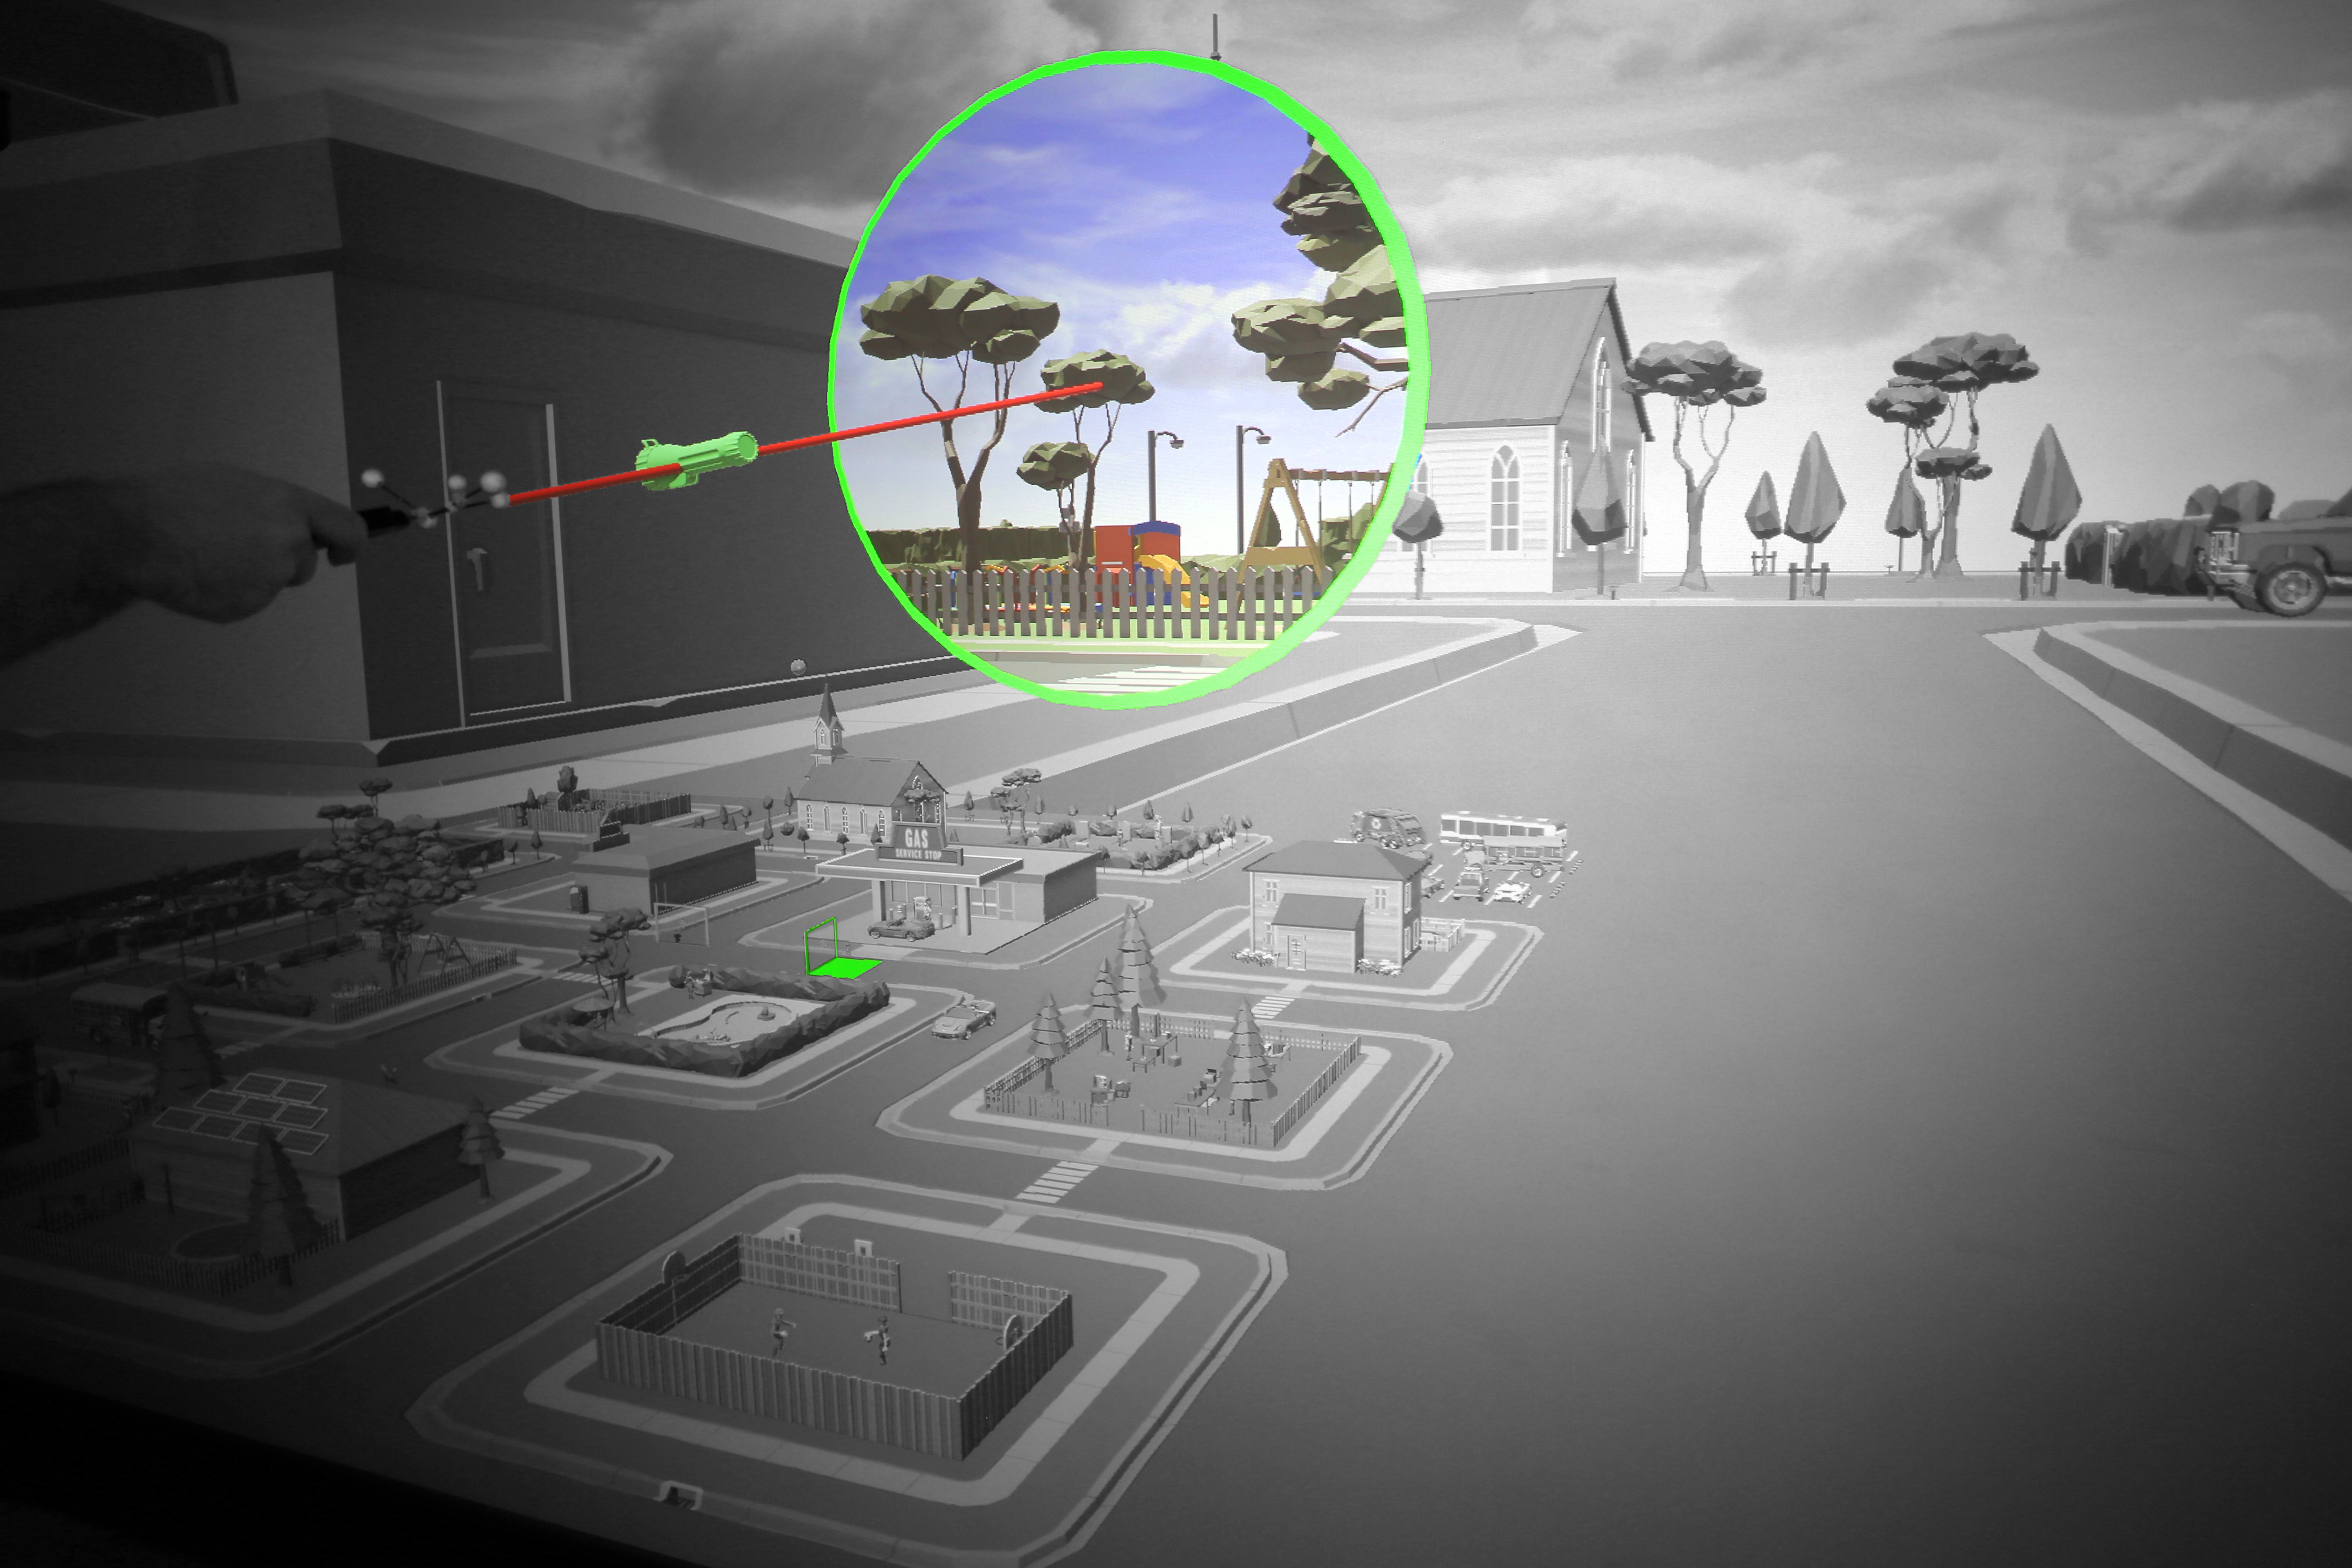
\includegraphics[width=0.8\textwidth]{images/peephole.jpg}
  \caption{Sobald die geplante Position bestätigt wurde erscheint über der grünen Plattform eine Taschenlampe. Greift man diese, erstellt man damit ein Guckloch, welches den Blick auf den Ort nach dem Teleport zeigt.}
  \label{fig:todo}
\end{figure}

Eine Möglichkeit wäre, dass das (in diesem Fall kugelförmige) Portal nach der Zielbestätigung direkt über der WIM bzw. dem gewählten Punkt erscheint. In diesem Fall wäre der Einstieg durch ein Aufblähen der Kugel denkbar.
Auch vorstellbar wäre, wie bei \cite{Kunert2014Photoportals}, das (in diesem Fall zwei- oder dreidimensionale) Fenster an eine Portalkamera oder seinen Pointer zu binden, sodass ein Nutzer, indem er seinen Kopf hineinsteckt, die neue Perspektive vor dem eigentlichen Teleport erkunden kann. Hierbei stellt sich aber der Einstieg problematisch dar: Es ist gut möglich, dass das Fenster von anderen Nutzern kaum oder nicht gesehen wird und eine Transition unvermittelt kommen kann.
Dies gestaltet sich einfacher, wenn das (in diesem Fall eher zweidimensionale) Fenster mittig, zentral und für alle sichtbar auf der Leinwand platziert wird (vgl. Galerie-Modus \cite{Kunert2014Photoportals}). So können  alle Nutzer das Fenster sehen und sind auf den Teleport, welcher durch Vergrößerung des Lochs stattfindet, vorbereitet.
Vor allem in diesem Fall stellt sich aber die Frage, ob dieses Portal sofort nach dem Platzieren der Miniaturplattform erscheinen soll. Es ist nämlich möglich, dass das Portal anderen Nutzern, die ggf. in diesem Moment die Umgebung erkunden die Sicht auf Dinge verdeckt. In einem solchen Fall sollte das Portal nicht sofort Erscheinen und im Zweifelsfall von jedem Nutzer wieder entfernt werden können.

Als Lösung für diese Problematik wurde die Funktion des Strahlwerkzeugs erweitert, damit ein solches \glqq Guckloch\grqq{} erzeugt und bewegt werden kann.
Zeigt der Nutzer mit seinem (ins unendlich verlängerten) Strahl in die WIM, so stehen ihm die oben aufgezählten Platzierungswerkzeuge zur Verfügung. Platziert er nun die (grüne) Plattform in der WIM so erscheint über dieser eine Taschenlampe, welche gegriffen werden kann. Richtet man diese Taschenlampe nun gegen die Leinwand, erscheint das Portal, wobei wie bei einem Taschenlampenkegel der Durchmesser dieses Lochs durch die Distanz der Taschenlampe zur Leinwand bestimmt wird. Will nun ein anderer Nutzer dieses Loch wieder aus seinem Sichtfeld entfernen, kann er mit seinem Strahl auf dieses zeigen, wobei dieser automatisch verlängert wird, wenn der Nutzer nicht mehr in die WIM zeigt. Dabei verschwindet die blaue Plattform vom Ende des Strahls. Der Nutzer kann dieses Loch nun selektieren und, während er den Button gedrückt hält, dieses an eine andere Stelle bewegen bzw. einfach außerhalb der Leinwand ziehen, woraufhin dieses verschwindet.
Klickt einer der Nutzer kurz auf das Loch so öffnet sich dieses wie beschrieben.

\section{Skalierung nach Teleport}
Im Rahmen der Technik ist es grundsätzlich möglich, die Skalierung der Nutzer in der Welt zu vergrößern bzw. zu verkleinern. Dies ermöglicht, dass Nutzer auch kleine Merkmale der Umgebung bis im Detail erkunden können oder durch Aufskalierung die Umgebung besser überblicken können. Dabei stellt sich die Frage, ob die aktuell gewählte Skalierung nach dem Teleport beibehalten werden soll oder ob man nach jedem Sprung wieder auf die Ausgangsgröße zurückskaliert wird. Beide Vorgehensweisen sind je nach Aufgabe und Motivation legitim. Für das Beispiel der virtuellen Stadtführung sind zum Beispiel beide Ausführungen denkbar. Entweder will der Stadführer, nachdem die Gruppe auf die Größe mehrerer hundert Meter vergrößert wurde, um eine schöne Aussicht über die Dächer der Stadt zu erhalten, diese nach dem Teleport beibehalten oder beim Besuch der nächsten Stadt wieder - in Menschengröße - zwischen den Straßenschluchten stehen.

\section{Steering Navigation}

\begin{figure}[h!]
  \centering
  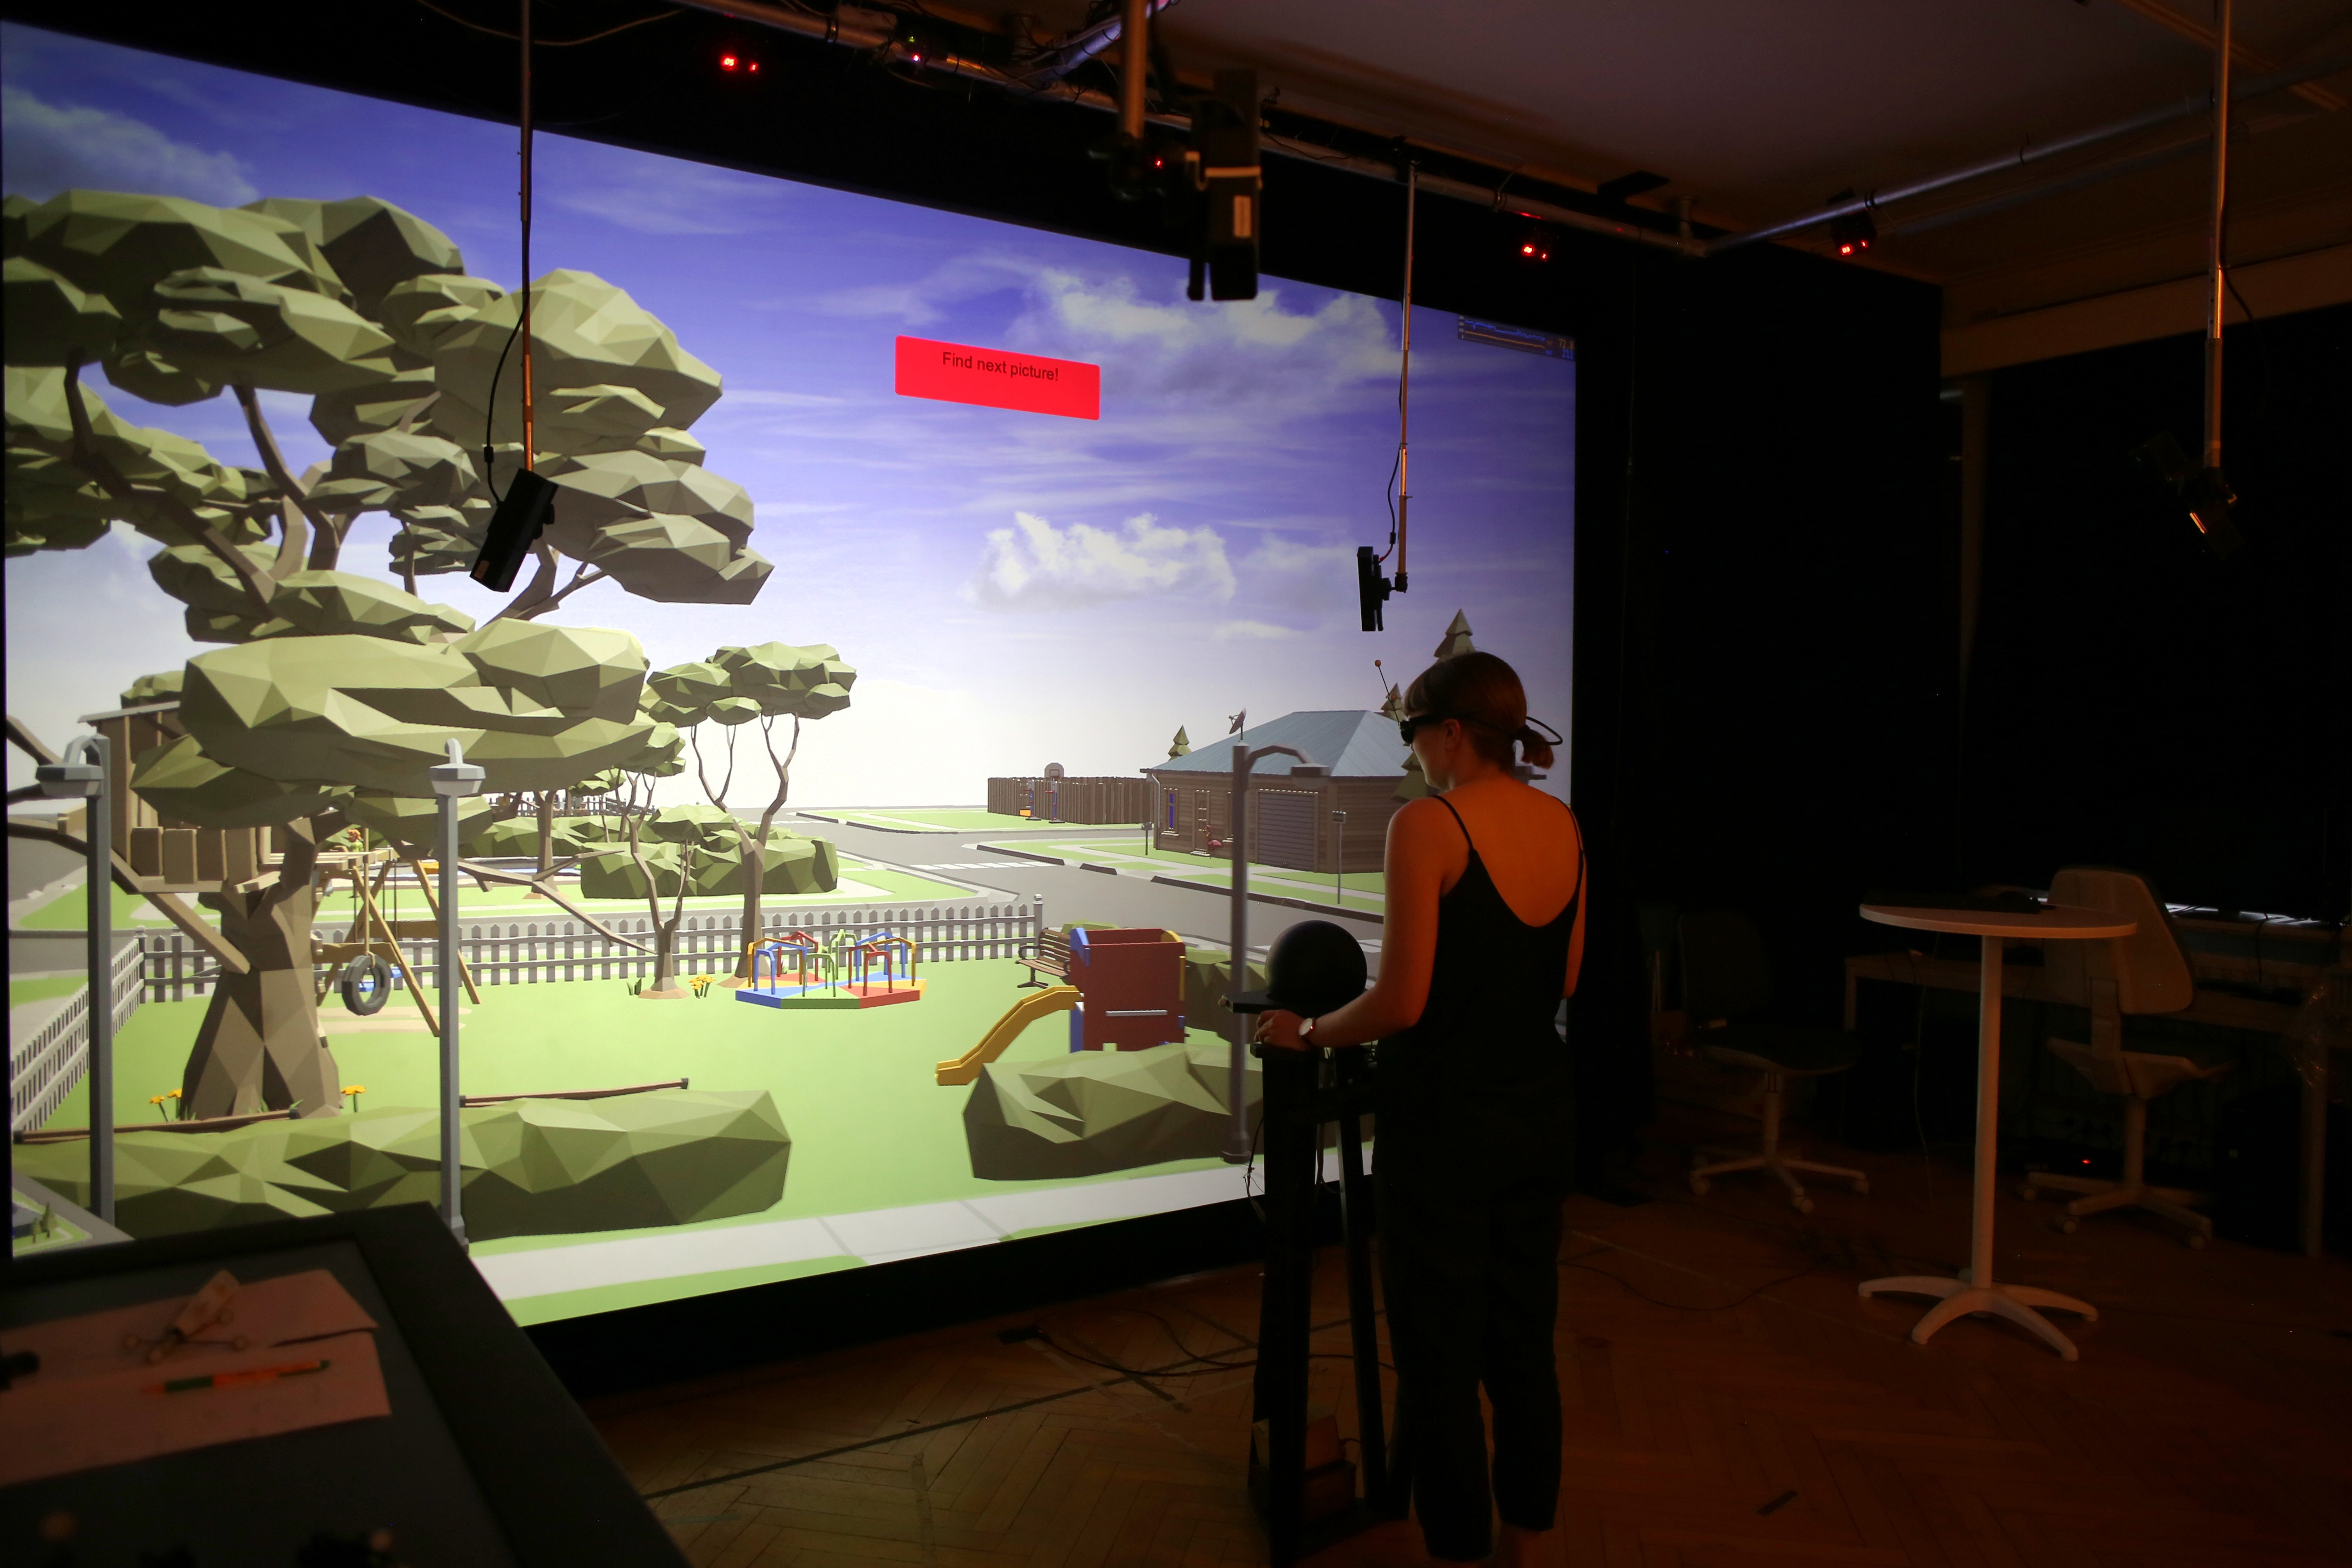
\includegraphics[width=0.8\textwidth]{images/steering.jpg}
  \caption{Zum Nachjustieren bietet das System Steering Navigation.}
  \label{fig:todo}
\end{figure}


Obwohl im besten Falle die Teleportationstechnik ausreicht, um ein Ziel zu erreichen, wird zusätzlich eine Möglichkeit zur Steering-Navigation angeboten. Dabei dient ein Spheron als 6-DOF Eingabegerät (vgl. \cite{Kulik2011C1x6}), mit dem man sich über kurze Distanzen (z.B. zum Nachjustieren nach dem Teleport) navigieren kann.

\section{Finales Interaktionsdesign}
Zur Durchführung einer Studie (mit jeweils zwei Nutzern) wurde folgendes Interaktionsdesign umgesetzt:
Um eine möglichst einfache und für alle sichtbare Interaktion mit der WIM zu ermöglichen, wurde die WIM auf eine feste Höhe von 1.30 Metern kurz vor der Leinwand platziert. Das Entkoppeln, sodass man sie in der Hand halten kann, wurde deaktiviert, da dies einerseits durch zahlreiche Drehungen die Raumwahrnehmung verschlechtern kann, andererseits sollten die Interaktionsmöglichkeiten nicht zu umfangreich sein, um unerfahrene Nutzer nicht zu überfordern. Die anfängliche Größe der WIM liegt bei 1.20 Metern, wobei die Nutzer diese wie oben beschrieben ändern können.
Die WIM ist mit Hilfe einer \textit{Spacemouse} drehbar, jedoch wird die WIM bei jedem öffnen und nach jedem Teleport wieder mit Norden nach oben ausgerichtet.
Dies soll dazu beitragen, dass Nutzer sich ein besseres räumliches Verständnis aneignen können (vgl. Kapitel 5).
Jeder der Nutzer besitzt ein Werkzeug, mit dem er die Technik bedienen kann. 
Für die Platzierung am Boden wird (neben der "Direkten Auswahl" (s.o.)) nur die Methode genutzt wird, erst den POI auszuwählen, dann Plattform in Blickrichtung dessen zu positionieren. Auch hier war der Grund, dass die Nutzer nicht mit zu vielen Möglichkeiten konfontiert werden sollen und diese Methode in Vortest als angenehmer eingeschätzt wurde.
Auch die Möglichkeit Planes of Interest zu platzieren wurde im Zuge dessen deaktiviert. Es kann immer nur eine Instanz der grünen finalen Plattform geben, aus der immer nur eine Portal erzeugt werden kann.
Bei jedem neuen Setzen verschwindet das Portalfenster.
Da in unserem beispielhaften Studiendesign ausschließlich Ziele am Boden bereist werden, wird statt der WIM eine unsichtbare Bodenplatte geschnitten, damit nicht durch Fehleingaben aus Versehen die Plattform auf Dächern oder Hecken gesetzt wird.
Bis auf die Skalierung der WIM werden alle Interaktionen durch die Verwendung eines einzigen Knopfes durchgeführt.
Die Skalierung der Nutzergruppe wird in der Studie nicht verändert, da alle zu bereisenden Ziele in der Skalierung eins zu eins aufzusuchen sind.
Zusätzlich zur Teleportationstechnik steht den Nutzern der Spheron zum Nachjustieren nach dem Teleport zur Verfügung. Grundsätzlich ist es aber aufgrund der vorher festgelegten Ziele nicht notwendig diesen auch zu nutzen, da alle Ziele mit der Teleportationstechnik alleine gefunden werden können.

\chapter{Evaluierung}
\section{Metriken}
Um die nun implementierte Technik zu evaluieren, müssen die im dritten Kapitel genannten Metriken genauer analysiert werden. Deswegen soll ein Blick in verwandte Arbeiten der letzten Jahre Hinweise darauf geben, wie diese Metriken in anderen Arbeiten quantifiziert wurden und ob bzw. wie eine ähnliche Vorgehensweise in unserem Fall angewendet werden kann.

\subsection{Bearbeitungszeit}
Selbstverständlich ist die Effizienz ein Kriterium, welches implizit in jeder Arbeit berücksichtigt wird, da eine schnelle und effektive Navigation immer ein wichtiges Ziel einer jeden Technik ist. Wenn dies überhaupt explizit gemessen wurde, wurde dies in den meisten Fällen schlicht und einfach mit der Bearbeitungszeit erfasst, welche gegen die einer ähnlichen Technik verglichen wurde (\cite{Suma2010EvaluationEnvironments}, \cite{Kopper2006DesignEnvironments}, \cite{3_Pierce1997}, \cite{Wingrave2006OvercomingWIM}). 
Bei Pierce et al. (\cite{3_Pierce1997}) liegt der Schwerpunkt vor allem anderen auf diesem Punkt. So wird hier begründet, dass die Durchführungszeit auch andere Metriken parallel mit abfragt:

\begin{addmargin}[25pt]{0pt} 

\textit{“In addition, travel time indirectly measures how easily users of a technique can maintain their orientation, form and execute plans, and detect destination.”}\cite{3_Pierce1997}

\end{addmargin}

Doch bei der Entwicklung dieser Technik stellen sich zwei Problematiken, denn zum einen gibt es keine Technik, gegen die verglichen werden kann, zum anderen kann die Kommunikation zwischen Gruppenmitgliedern die resultierende Bearbeitungszeit negativ beeinflussen, obwohl sie ein Indikator für eine gut abgestimmte Reiseplanung sein kann.

Die Herangehensweise soll in diesem Fall also eine andere sein:
Die Navigation durch Platzieren der Nutzerplattform in der WIM kann analog zu den Platzierungsaufgaben mit einem Stift, bzw. mit Lochscheiben und Steckstiften in den frühen Studien von Paul Fitts \cite{fitts1954information} in einem dreidimensionalen Interface aufgefasst werden. Die Anwendbarkeit seines Modells auf zwei- und dreidimensionale virtuelle Umgebungen wurde in unzähligen Folgestudien nachgewiesen (\cite{mackenzie1992fitts}, \cite{drewes2010only}, \cite{zhai2004characterizing} für einen Überblick der Forschung).

Fitts' Gesetz beschreibt die lineare Abhängigkeit der benötigten Zeit (MT) von einem
Schwierigkeitsindex (ID), der sich wiederum aus der Zielentfernung (D) und Zielgröße (W) ableiten lässt ($ID=log_2(2D/W)$).

Fitts testete Schwierigkeitsindizes zwischen 1 und 10. Seine Teilnehmer benötigten dafür je nach Schwierigkeit zwischen 180 und 1100 ms \cite{fitts1954information}. An Computerarbeitsplätzen ist die Effizienz der Zielbewegungen typischerweise etwas schlechter (z.B. \cite{Forlines}, \cite{mackenzie1992fitts}, \cite{MacKenzie:2008:FTS:1357054.1357308}, \cite{Wobbrock:2008:EMP:1357054.1357306}), vor 
allem im Falle von 3D Zielbewegungen in virtuellen Umgebungen in denen kein taktiles Feedback verfügbar ist (z.B. \cite{arsenault2004importance}, \cite{grossman2004pointing}, \cite{teather2011pointing}, \cite{lubos2014analysis}).

Basierend auf den oben erwähnten Forschungsergebnissen entschieden wir
uns, dass der maximale Schwierigkeitsindex (ID) der motorischen
Interaktionsbewegungen bei der Nutzung unserer Technik nicht höher als 5 sein sollte, um Ineffizienz und Frustration zu vermeiden. Offenbar benötigen Nutzer auch für 3D Selektionsaufgaben mit etwas geringeren IDs schon etwa zwei Sekunden. Im
Zusammenhang mit einer Zielentfernung von einem Meter, was in etwa der Distanz, die man angenehm durch Ausstrecken des Armes erreichen kann entspricht, ergibt sich daraus eine minimale Zielgröße von etwa 5 bis 6 cm. Dies wiederum entspricht bei der gewählten Skalierung (1:100) der WIM einer Genauigkeit von (+/-) 2,5 bis 3,0 Metern, mit denen die miniaturisierte Plattform innerhalb von ca. 2 Sekunden platziert werden kann.



\subsection{Genauigkeit}
Die Genauigkeit ist stets mit der resultierenden Distanz zwischen Position des Nutzers nach der Navigation und eines im Vorhinein festgelegten Ziels zu bestimmen. 
Explizit wird dies beispielsweise in \cite{Krekhov2018GulliVR} abgefragt: Bei der \textit{“Aiming”} genannten Technik soll der Nutzer in einem Zielgebiet landen, welches durch eine farbige Zielscheibe gekennzeichnet ist. Die durchschnittliche Distanz zum Bullauge ist dabei das Maß, welches die Genauigkeit bestimmt.
Wichtig zu erwähnen ist, dass die Genauigkeit in den meisten Fällen mit der Bearbeitungszeit zusammenhängt: Hat man mehr Zeit oder nimmt man sie sich, so ist in den meisten Fällen die Genauigkeit größer (vgl. dazu auch vorheriger Unterpunkt!).
So wird in manchen Arbeiten (\cite{BowmanTestbedTechniques}, \cite{3_Pierce1997}) eine bestimmte Genauigkeit vorausgesetzt, in dem man sich innerhalb eines bestimmten Radius zum Ziel befinden muss, damit die Reise als abgeschlossen zählt.
Die Genauigkeit so exakt zu quantifizieren ist in unseren Augen allerdings nicht zwangsläufig notwendig und wird durch den Fitt's Task hinreichend abgedeckt. 
Viel wichtiger, als möglichst nahe an einem vorher festgelegten Punkt zu landen, ist unserer Meinung nach, dass das gewünschte Ziel vollständig sichtbar ist. 
Deshalb erhalten die Nutzer in unserer Studie Bilder von Objekten, die sich in der zu bereisenden Umgebung befinden, welche sie so ansteuern müssen, dass alle Details auf dem Bild auch in ihrer Perspektive zu sehen sind.

Ein weiteres Kriterium, mit dem die Genauigkeit ebenfalls gemessen werden kann ist die Häufigkeit von Kollisionen mit der virtuellen Umgebung(vgl. \cite{Suma2010EvaluationEnvironments}). Da unsere Technik die Möglichkeit bietet, die Nutzerplattform so zu platzieren, dass Kollisionen im Vorhinein ausgeschlossen werden und eine zukünftige Weiterentwicklung der Technik eine Kollisionsabfrage beinhalten könnte, soll dieses Kriterium nicht weiter abgefragt werden.


\subsection{Informationsaufnahme}
Mit der Aufnahme von Informationen beschäftigen sich Suma et al. \cite{Suma2010EvaluationEnvironments}. Sie schlagen dabei verschiedene Möglichkeiten vor:


\textbf{Objekterkennung:}\\
Der Nutzer erhält eine Liste von 36 Objekten, von denen er die Hälfte auf seiner Reise sehen konnte. Die andere Hälfte war nicht in der virtuellen Umgebung platziert. Er erhält 8 Minuten Zeit, die Objekte mit “War in der Umgebung” und “War nicht in der Umgebung” zu klassifizieren. In der Evaluierung werden die False Positives werden von den Correct True Positives abgezogen und es ergibt sich somit ein Score von 0 - 18.


\textbf{Objektplatzierung:}\\
Der Nutzer erhält eine Karte der von ihm bereisten Umgebung sowie eine nummerierte Liste mit allen 18 Objekten, die in der Umgebung platziert waren. 
Er wird gebeten, die Nummer aller Objekte an der Stelle in der Karte einzutragen, an der er sie gesehen hat (oder gemeint gesehen zu haben).
Das Ergebnis wird im Folgenden von einer Drittperson geprüft und bewertet.
Dabei wird jedes richtig platzierte Objekt mit einem Punkt gewertet und es ergibt sich auch hier ein Score von 0 - 18. 

Die Objekterkennung wird in unserem Fall nicht abgefragt, da die Nutzer nur Teile der Karte bereisen und sich dabei auf das Finden der Bilder konzentrieren, sodass der Fokus auf einem anderen Task liegt und etwaige Objekte übersehen werden können.
Die Objektplatzierung allerdings wird allerdings auch in unserem Fall vorgenommen. Dabei werden den Nutzern, nachdem sie die Karte bereist haben und alle Bilder gefunden haben, diese Bilder erneut ausgehändigt, sowie eine Karte, die nur die Umrisse der bebauten "Inseln" sowie die Kirche als Orientierungspunkt zeigt (vgl. Abbildung).
In dieser sollen die Nutzer dann die Bildnummern, sowie die Blickrichtung in Form eines Pfeils einzeichnen.


\subsection{Nutzerkomfort:}
Um den Nutzerkomfort zu messen wird neben generellen Fragen zum Wohlbefinden in der Mehrzahl aller Arbeiten (z.B. \cite{Krekhov2018GulliVR}, \cite{Suma2010EvaluationEnvironments}, \cite{Usoh1999WalkingEnvironments}) der Simulator Sickness Questionnaire genutzt (\cite{Kennedy1993SimulatorSickness}). Dieser fragt das generelle Wohlbefinden nach dem Aufenthalt in einer Simulation bzw. in unserem Fall nach der Navigation in einer Simulation ab.

Auch in unserem Fall soll die Technik so entwickelt werden, dass durch sie keine merkliche Verschlechterung des allgemeinen Wohlbefindens der Nutzer eintritt. Dieses wird durch das Durchführen des SSQ vor und nach jedem Durchlauf der Studie ermittelt, wobei sich der Wert nicht oder kaum (hier noch eine Zahl?) verschlechtern dürfte, da unsere Technik wie bereits beschrieben mit einem minimum an Steering und Motionflow auskommt.

\subsection{Raumwahrnehmung}
Die Raumwahrnehmung der Nutzer wird häufig (z.B. \cite{Kopper2006DesignEnvironments}, \cite{Richardson1999}) abgefragt, indem der Nutzer die Himmelsrichtung zu einem anderen, schon bekannten Ort anzeigen muss. Hierfür wird der angezeigte Winkel von dem tatsächlichen Winkel subtrahiert, um die tatsächliche Abweichung zu bestimmen (“Pointing error”). \cite{Kopper2006DesignEnvironments} beschreibt dies anders als nach Bowmans Metriken als “Accuracy”.
In der Arbeit von Vuong \cite{29_POINTING_ERROR_jennyVuong_small}, S.23 werden aus verschiedenen Studien in virtuellen Umgebungen solche resultierenden Abweichungen zusammengefasst. Die meisten dieser Abweichungen liegen im Gebiet von 10 bis 40 Grad.
Ein Beispiel davon ist die Arbeit von Thorndyke et al. \cite{Thorndyke1980LNAVIGATION}, in welcher ein Experiment durchgeführt wird, in dem Testpersonen sich eine Umgebung durch Navigieren oder dem Lernen einer Karte merken sollen und dieses Wissen im Folgenden abgefragt wurde.
Die (in diesem Fall nicht virtuelle) Umgebung ist dabei ein Stockwerk eines Gebäudes. Die Testpersonen wurden in zwei Gruppen aufgeteilt: Diejenigen, die die Karte des Stockwerks intensiv (bis sie  lernen und diejenigen, die das Stockwerk durch Navigieren in diesem gelernt haben, da sie unterschiedliche Zeitdauer dort gearbeitet haben ( “1 to 2 months, 6 to 12 months, or 12 to 24 months”).
In verschiedenen Experimenten mussten sie u.a. die Richtungen anderer Räume anzeigen.
Die Ergebnisse dabei sahen wie folgt aus: 
\begin{addmargin}[25pt]{0pt} 

\textit{Map learner: $\approx 39 ^\circ$ \\
1-2 months experience: $\approx  25 ^\circ$ \\
6-12 months experience: $\approx  24 ^\circ$ \\
12-24 months experience: $\approx  19 ^\circ$ \\}
\end{addmargin}

Weißker \cite{Weibker2018SpatialEnvironments} vergleicht in seiner Arbeit die Abweichungen die durch Steering und Teleportations Navigation entstehen. In diesem Falle liegen die Abweichungen im Durchschnitt knapp unter 20 Grad.

Auch nach dem Nutzen unserer Technik sollen die Testpersonen eine Vorstellung der Umgebung haben, welche sie bereisen. Dies soll abgefragt werden, in dem die Nutzer nach jeder Reise die Richtung anzeigen, in der sie den zuletzt besuchten POI (also das letzte Bild) vermuten. Wie oben beschrieben wird daraus die Abweichung in Grad berechnet. 
Die Ergebnisse von Thorndyke und Weißker legen nahe, dass die durchschnittliche Abweichung zwischen 20 und 40 Grad liegen wird. Das Ziel der Technik wird also sein, diesen Wert möglichst nahe an 20 Grad anzunähern und einen Wert von über 40 Grad zu vermeiden.

Suma et al. (\cite{Suma2010EvaluationEnvironments}) lassen zur Bewertung der Raumwahrnehmung die Nutzer einen Sketch der Karte erstellen und diese von Dritten auf einer Skala von 1 - 5 bewerten. Hierbei wird selbstverständlich nur die Struktur der Karte und nicht die Zeichenqualität bewertet.
Das vollständige Zeichnen der Karte stellte sich aufgrund der Größe in Vorstudien als nicht praktikabel dar. Jedoch kann das Einzeichnen der bereisten Orte (siehe 9.1.3) ebenfalls als Abfrage der Raumwahrnehmumg
aufgefasst werden.

\subsection{Nutz- und Lernbarkeit}
Die System Usability Scale (SUS)\footnote{https://www.usability.gov/how-to-and-tools/methods/system-usability-scale.html}
bietet eine schnelle und leichte Möglichkeit, die Nutzbarkeit eines Systems zu evaluieren. Studienteilnehmer erhalten einen Fragebogen mit 10 Punkten (z.B. “I think that I would like to use this system frequently.”), wobei diese jeweils mit einem Score von 0 - 4 bewertet werden. Diese werden zusammengezählt und mit 2.5 multipliziert, was in einem Wert zwischen 0 und 100 resultiert.

Die Technik soll daher in unserem Fall einen Wert erreichen, der in diesem SUS nicht unter 70 liegt. Weiterhin soll die Technik so intuitiv sein, dass die Nutzer nach kurzer Vorführung (also nach zwei bis drei Navigationsvorgängen) durch den Versuchsleiter, selbst in der Lage sind, sich einigermaßen sicher und ohne weiter Anleitung zu navigieren. Im Rahmen der Auswertung der Photoportale \cite{Kunert2014Photoportals} wurde festgestellt, dass eine Vielzahl von Knöpfen an einem Eingabegerät zur einer steileren Lernkurve führt, weswegen die Technik, wie bereits erwähnt, mit einem einzigen Knopf bedienbar ist.


\subsection{Präsenz}
Um das Gefühl der Präsenz des Nutzers ab zu fragen, schlagen Krekhov et al. \cite{Krekhov2018GulliVR} eine Kombination aus dem “Igroup Presence Questionnaire” \cite{witmer1998measuring} und dem Presence Questionnaire(\cite{schubert1999}) vor:

\begin{addmargin}[25pt]{0pt} 

\textit{By focusing more on the interactions with and navigation
through the game environment, the PQ is a good complement
of the IPQ to assess all aspects of presence.
}\cite{Krekhov2018GulliVR}

\end{addmargin}

Beide evaluieren verschiedene Aspekte der Präsenz und des Realismusgefühls durch Fragen, welche man mit Hilfe einer Likert Skala bewertet.

In unserem Fall wird zwar keine direkte Abfrage des Präsenzgefühls vorgenommen, dennoch soll die Technik zu jederzeit einen konsistenten Fluss bieten und das Immersionsgefühl soll zu keinen Moment eingeschränkt werden.

\subsection{Gruppeninteraktion}
Kollaboration und Gruppeninteraktion lassen sich schlecht mathematisch messen. 
Stattdessen sollen drei Kriterien als Maßstab für die Nutzbarkeit in einer Gruppe dienen.
Beobachtbarkeit, Umkehrbarkeit und Unterbrechbarkeit.
Auch in diesem Fall sollen drei Fragen zur Abfrage dieser Kriterien dienen, welche von 0 bis 4 bewertet werden:

\textit{Hattest du zu jederzeit das Gefühl, an der Planung und Durchführung der Navigation beteiligt sein zu können?}

\textit{Hattest du das Gefühl, dass alle Mitglieder zu jeder Zeit das Ziel der Reise kannten?}

\textit{Hattest du das Gefühl, den Navigationsvorgang zu jeder Zeit abbrechen zu können, wenn du mit diesem nicht einverstanden warst?}

\section{Studiendurchführung}
\subsection{Teilnehmer}
Zur Durchführung der Studie wurden insgesamt XXX Gruppen bestehend aus je zwei Personen eingeladen. XXX der Teilnehmer waren männlich, XXX weiblich.

\subsection{Vorgehen}
Zu Beginn werden die Teilnehmer etwa 10 Minuten lang in das System eingeführt, wobei ihnen alle notwendigen Funktionen vorgestellt und gezeigt wurden.
Infolgedessen wird zuerst der SSQ ausgefüllt und die Nutzer erhalten das erste Bild, welches es zu finden gilt. Nachdem sie die richtige Position in der WIM gefunden haben und den Teleport durchgeführt haben, wird die WIM ausgeblendet und der aktuelle Ort geloggt. Daraufhin wird abgefragt, ob sie sich erinnern können, in welcher Richtung der zuletzt bereiste Ort liegt. Für den Fall, dass sie sich sicher sind, soll der Pointer in die Höhe gehalten werden beziehungsweise nach unten, falls sie sich unsicher sind. Auch diese Sicherheit wird geloggt, bevor die Nutzer die tatsächlich vermutete Richtung durch eine Geste mit dem Pointer anzeigen. \textbf{Durch das vorherige Anzeigen der Sicherheit können im folgenden Ergebnisse, bei denen sich ein Nutzer nur an der Zeigerichtung seines Partner orientiert, herausgerechnet werden.}
Wenn das Team die Zeigerichtungen bestätigt, wird die tatsächliche Abweichung jedes Nutzers geloggt und die WIM wird wieder sichtbar. Die Nutzer erhalten ein neues Foto und starten den Durchlauf erneut.
Insgesamt mussten die Nutzer XXX Fotos in der Karte finden.
Nachdem diese alle gefunden wurden, wird erneut der SSQ sowie der SUS und der RAW-TLX ausgefüllt.
Als letzten Schritt erhalten die Nutzer die Karte mit den Umrissen der Inseln, sowie alle bereisten Bilder und sollen dabei die Nummern und Blickrichtung der Bilder in die Karte eintragen. 


\chapter{Evaluierung}
\input{text-source/platzhalter.tex}

\chapter{Diskussion}
\input{text-source/platzhalter.tex}

%%%%%%%
% Conclusion and Future Work
%%%%%%%

\chapter{Fazit und Ausblick}
Im Rahmen dieser Arbeit wurde eine intuitive Technik entwickelt, mit denen es mehreren Nutzern im Leinwandsetup möglich ist, effizient durch eine virtuelle Umgebung zu reisen. 

Die Studie hat gezeigt, dass ...


Ein zentraler Punkt, der die Nutzbarkeit der Technik noch verbessern würde, wäre die Implementierung eines Kollisionsschutzes beim Platzieren der Nutzerplattform in der WIM. Dies könnte im ersten Schritt dadurch verwirklicht werden, dass die Plattform eingefärbt wird und nicht platzierbar ist, wenn sich einer der Nutzer in bzw. hinter einer Wand oder ähnlichem befindet. Dies könnte weiterhin durch eine Art \glqq Snapping\grqq{}-Mechanismus erweitert werden, welcher die Plattform stattdessen automatisch in einer möglichen Ausrichtung dreht, die der aktuell angezeigten am nächsten ist.
Auch sind weitere Platzierungsmechanismen denkbar. So wäre zum Beispiel. eine Interaktionstechnik nach dem Vorbild der Navidget-Technik \cite{HACHET2009225} denkbar, um POI's leichter aus verschiedenen Winkeln betrachten zu können. Grundsätzlich ähneln sich die beiden Techniken nämlich in der Hinsicht des Planens einer gewünschten Kameraorientierung. Die Platzierung in der WIM bringt dabei den Vorteil mit sich, dass man auch außerhalb des aktuellen Sichtfelds navigieren kann, wobei die Ausrichtung entlang der Kugelnormalen wie bei Navidget in manchen Fällen ein Verrenken des Handgelenks verhindern kann.

Auch denkbar wäre beim Vorgang des Platzierens die Skalierung der Nutzer, die in unserem Fall immer auf eins zu eins zurückgesetzt wurde, festzulegen. Wie eine entsprechende, intuitive Festlegung der Skalierung zu bewerkstelligen wäre, müsste im Rahmen einer anderen Arbeit geklärt werden.

Bei dem Erzeugen des Portalfensters wäre außerdem denkbar, dieses, angelehnt an die Photoportale, erst am Pointer desjenigen anzuzeigen, der die Plattform in der WIM platziert hat, bevor dieser sie für alle zugänglich an die Leinwand strahlt.
Auch, wenn diese Technik im Hinblick auf Mehrbenutzerszenarien entwickelt wurde, ist eine Nutzung dieser im Einzelnutzerbereich sehr gut denkbar. So könnte ein Nutzer mit HMD auf Knopfdruck die WIM in seiner nicht-dominanten Hand aufrufen und sich selbst in dieser platzieren. Denkbar wäre dabei zum Beispiel, dass der Nutzer sich in einer transparenten \glqq Seifenblase\grqq{} befindet, welche dieser mit Hilfe des sich gerade verbreitenden Fingertrackings ganz natürlich anfassen und in die WIM stellen kann. Auch hier könnte der Nutzer mit einem Loch in dieser \glqq Seifenblase\grqq{} in die neue Welt schauen, welche auf Knopfdruck analog zu unserer Technik \glqq aufplatzt\grqq{}. Im Einzelnutzerbereich mit HMD kommt einem außerdem die StepWIM\cite{Stoakley2010VirtualWIM} wieder in den Sinn:
Hier wäre es gut denkbar, den Boden innerhalb des Trackingspaces auf Knopfdruck durch die WIM zu ersetzen, in der man sich, nachdem man zum gewünschten Reiseziel gelaufen ist, mit einer entsprechenden Selektionstechnik, ähnlich wie in unserer Implementierung, platzieren kann.
Hiermit wäre man nahe an der Implementierung von \cite{Krekhov2018GulliVR}, würde sich allerdings den (eigentlich unnötigen) Aufskalierungsvorgang sparen.

Die zentrale Einschränkung der hier vorgestellten Technik stellt allerdings da, dass man aktuell nur Gebiete in Größe einer Nachbarschaft effizient bereisen kann. Eine Implementierung, mit denen man sein Ziel auch in anderen Städten und Gebieten wählen kann ist für wirklich große Distanzen unumgänglich. Wie bereits beschrieben wäre dafür die Baumtraversion von \cite{pierce_representations} oder ein Vorgehen wie bei \cite{wingrave2006overcoming} bei dem man die WIM noch besser skalier- und scrollbar macht, wäre denkbar.



\chapter{Tools}

\vspace{0.5cm}

\begin{figure}[]
  \centering
  
\includegraphics[width=0.5\textwidth]{images/todo.png}
  \caption{This is an example ToDo picture.}
  \label{fig:todo}
\end{figure}

Hypotheses and sub-hypotheses can be formulated like this:

\begin{hypothesis}
\label{hyp:test}
This is a hypothesis.
\end{hypothesis}

\begin{shypothesis}
\label{shyp:test}
This is a sub-hypothesis.
\end{shypothesis}

Hypothesis \cref{hyp:test} is very importance and must be referenced in the text.



Wie im zweiten Kapitel beschrieben, lassen sich durch die Größe der WIM mit Hilfe Fitt`s Law implizit Rückschlüsse auf das Kriterium der Bearbeitungszeit ziehen. Da der Teleport selbst nämlich keinerlei Zeit in Anspruch nimmt, bestimmt die Zeit zur Zielauswahl in der WIM die Dauer der Reise. Diese muss also möglichst gering gehalten werden. In diesem Falle wird wie bereits beschrieben ein maximaler Index of Difficulty von 5 vorausgesetzt, um eine zügige Interaktion zu gewährleisten. Diese wird Interaktion ist in Form von verschiedenen Auswahlstrahlen (genauer beschrieben im nächsten Unterpunkt) in der WIM jedoch eine einfache 3D-Zielbewegung mit fünf Freiheitsgraden für deren Effizienz umfangreiche wissenschaftliche Erkenntnisse vorliegen. Aus aktuelle Arbeiten zu 3D-Selektionsaufgaben (Teather und Stürzlinger (2011), Grossman und Balakrishnan (2004)) kann man für einen Schwierigkeitsindex von 4 eine Bearbeitungsdauer von ca. 2 Sekunden ableiten.




\def\rot{\rotatebox}

%https://tex.stackexchange.com/questions/98388/how-to-make-table-with-rotated-table-headers-in-latex
 \begin{table}[H]
 \centering
 \begin{tabular}{|c|l|r|r|r|r|}
 \hline
 & \multicolumn{1}{c|}{\rot{90.0}{Sichtbarkeit}} & \multicolumn{1}{c|}{Text} & \multicolumn{1}{c|}{Text} & \multicolumn{1}{c|}{Text} & \multicolumn{1}{c|}{text}\\
 \hline
 \parbox[t]{2mm}{\multirow{3}{*}{\rotatebox[origin=c]{90}{rota}}} & text &&&&\\
 & text &&&&\\
 & text &&&&\\
 \hline
 \end{tabular}
 \end{table}


%%%%%%%
% Biblography
%%%%%%%

{\footnotesize
\bibliography{other}{}
\bibliographystyle{ieeetr}
}

%%%%%%%
% Appendix
%%%%%%%

\appendix
\chapter{Appendix}
This is the appendix...



\end{document}